\documentclass[11pt,letterpaper]{article}

\usepackage{showlabels}
\usepackage{fullpage}
\usepackage{pslatex}
\usepackage{hyperref}
%\usepackage{latexsym}
\usepackage[english]{babel}
\usepackage[utf8]{inputenc}
\usepackage{amsmath}
\usepackage{bm}
\usepackage{graphicx}
\usepackage{tikz}
\usepackage{xcolor}
\usepackage{url}
%\usepackage[colorinlistoftodos]{todonotes}
\usepackage{rotating}
\usepackage{natbib}
\usepackage{amssymb}



\usepackage{caption}

\usepackage{tikz-dependency}
\usepackage{longtable}


\newcommand{\R}[0]{\mathbb{R}}
\newcommand{\E}[0]{\mathbb{E}}
\newcommand{\Ff}[0]{\mathcal{F}}

\usepackage{multirow}

\newcommand{\soft}[1]{}
\newcommand{\nopreview}[1]{}
\newcommand\comment[1]{{\color{red}#1}}
\newcommand\mhahn[1]{{\color{red}(#1)}}
\newcommand\note[1]{{\color{red}(#1)}}
\newcommand\jd[1]{{\color{red}(#1)}}
\newcommand\rljf[1]{{\color{red}(#1)}}
\newcommand{\key}[1]{\textbf{#1}}

\usepackage{amsthm}

\newcommand{\thetad}[0]{{\theta_d}}
\newcommand{\thetal}[0]{{\theta_{LM}}}

\newcounter{theorem}
\newtheorem{proposition}[theorem]{Proposition}
\newtheorem{thm}[theorem]{Theorem}
\newtheorem{corollary}[theorem]{Corollary}
\newtheorem{question}[theorem]{Question}
\newtheorem{example}[theorem]{Example}
\newtheorem{lemma}[theorem]{Lemma}



% https://tex.stackexchange.com/questions/24132/overline-outside-of-math-mode
\makeatletter
\newcommand*{\textoverline}[1]{$\overline{\hbox{#1}}\m@th$}
\makeatother

\frenchspacing
%\def\baselinestretch{0.975}

%\emnlpfinalcopy
%\def\emnlppaperid{496}

\title{Supplementary Information for: Modeling word and morpheme order in natural language as an efficient tradeoff of memory and surprisal}
\author{Michael Hahn, Judith Degen, Richard Futrell}

\begin{document}

\maketitle

\tableofcontents


%
%\begin{center}
%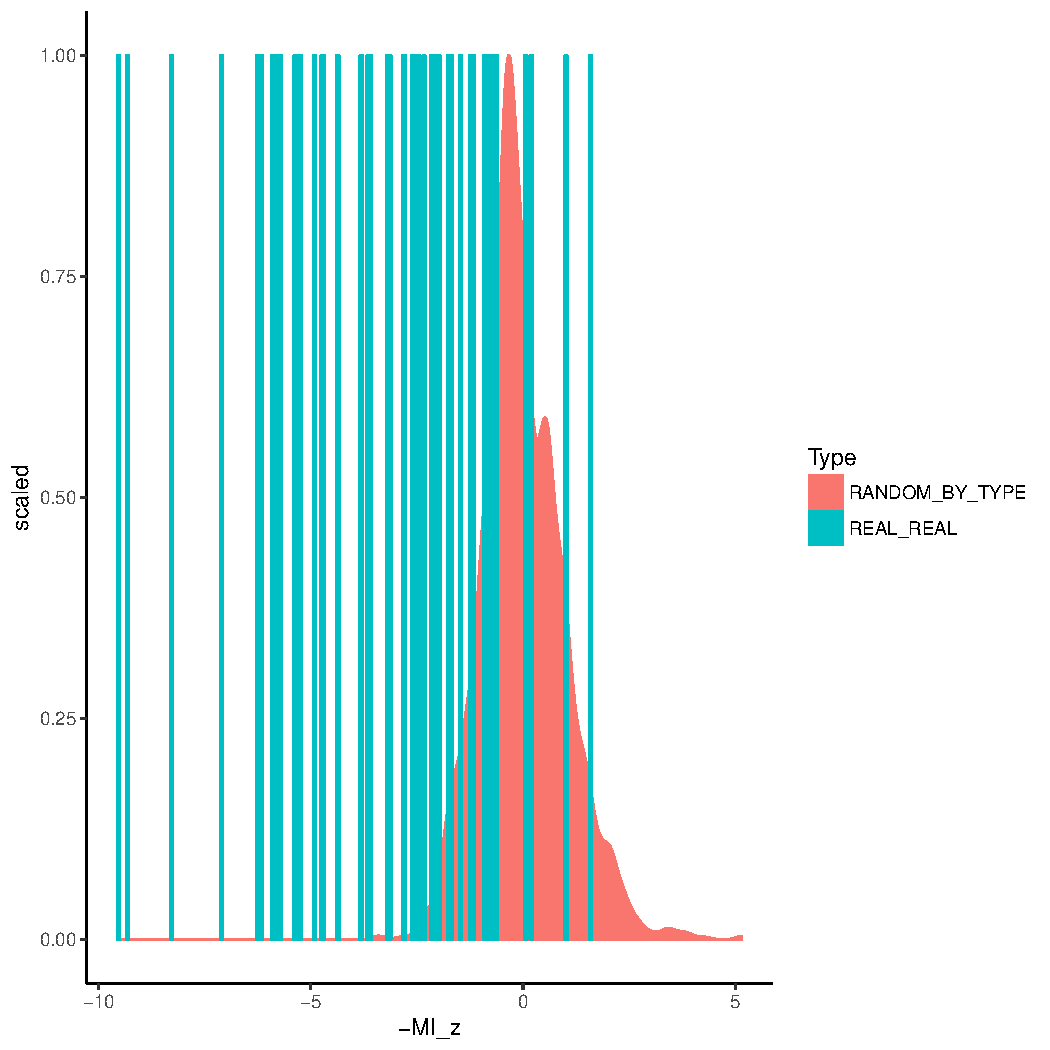
\includegraphics[width=0.5\textwidth]{../code/analysis/visualize_neural/figures/full-REAL-listener-surprisal-memory-HIST_z_byMem_onlyWordForms_boundedVocab.pdf}
%\captionof{figure}{Histogram}\label{fig:hist-real}
%\end{center}
%
%


\section{Formal Analysis and Proofs}

In this section, we prove the Information Locality Bound Theorem and related theoretical results referenced in the main paper.

\subsection{Mathematical Assumptions}\label{sec:math-assumptions}

We first make explicit how we formalize language processing for proving the theorem.
This is a formally fully rigorous statement of the model described in Section 3.1 of the main paper.


\subsubsection{Ingredient 1: Language as a Stationary Stochastic Process}
We represent language as a stochastic process of words $W = \dots w_{-2} w_{-1} w_0 w_{1} w_{2} \dots$, extending indefinitely both into the past and into the future \citep{doob1953stochastic}.
The symbols $w_t$ belong to a common set, representing the words or morphemes of the language.
Formally, a stochastic process is a probability distribution over infinite sequences $\dots w_{-2} w_{-1} w_0 w_{1} w_{2} \dots$ \citep{doob1953stochastic}.
As $t$ runs over the set of integers $\mathbb{Z}$, it will sometimes be convenient to write such an infinite sequence as $(w_t)_{t \in \mathbb{Z}}$.
This distribution gives rise to probability distributions over finite subsequences
\begin{equation}
	P(w_t, \dots, w_{t+T})
\end{equation}
for integers $t, T$, and to conditional probabilities
\begin{equation}
	P(w_t | w_{t-T}, \dots, w_{t-1})
\end{equation}
%where $w_{<t}$ stands for the semi-infinite sequence $\dots, w_{t-2}, w_{t-1}$.

\paragraph{Infinite Length}
We assume that the process $W$ extends infinitely into both past and future, whereas real words, sentences, and conversations are finite.
This is not a contradiction:
In Studies 1--3, we model $W$ as a sequence of independent sentences or words, separated with a special ``end-of-sentence'' symbol.
Modeling $W$ as such an infinite sequence of finite sentences provides a way to formalize the memory-surprisal tradeoff in a way independent of the time point $t$.

%It allows us to study the process $W$ without special consideration of what happens at the beginning or end of the sequence.


%The assumption of infinite length is for mathematical convenience, and does not affect the substance of our results:
%
%As we restrict our attention to the processing of individual sentences (Experiments 1 and 2) or individual words (Experiment 3), which have finite length, we do not actually make use of long-range and infinite contexts.

\paragraph{Stationarity}
We make the assumption that the process $W$ is \emph{stationary} \citep{doob1953stochastic}.
This means that the joint distribution of different symbols depends only on their \emph{relative positions}, not their \emph{absolute positions}.
Formally, this means that joint probabilities do not change when shifting all observations by a constant number $\Delta$ of time steps. That is, for any integers $t$, $\Delta$, and $T>0$:
\begin{equation}
	P(w_t, \dots, w_{t+T}) = 	P(w_{t+\Delta}, \dots, w_{t+T+\Delta})
\end{equation}
Informally, this says that the process has no `internal clock', and that the statistical rules of the language do not change over time at the timescale we are interested in.
In reality, the statistical rules of language do change: They change as language changes over generations, and they also change between different situations -- e.g., depending on the interlocutor at a given point in time.
However, we are interested in memory needs in the processing of \emph{individual sentences} or \emph{individual words}, at a timescale of seconds or minutes.
At this level, the statistical regularities of language do not change, making stationarity a reasonable modeling assumption.


The choice to model language as a stationary stochastic process is common to information-theoretic studies of text, including studies of entropy rate \citep{shannon1951entropy,bentz2017entropy,takahashi2018cross}, excess entropy~\citep{debowski-excess-2011,hahn2019estimating}, and mutual information~\citep{ebeling-entropy-1994,lin-critical-2017}.

\subsubsection{Ingredient 2: Postulates about Memory and Processing}
The second ingredient consists of the three postulates about memory and processing described in the main paper.
We repeat these here for reference:
\begin{enumerate}
    \item Comprehension Postulate 1 (Incremental memory). At time $t$, the listener has an incremental \key{memory state} $m_t$ that contains her stored information about previous words. The memory state is given by a \key{memory encoding function} $M$ such that $m_t = M(w_{t-1}, m_{t-1})$.
    \item Comprehension Postulate 2 (Incremental prediction). The listener has a subjective probability distribution at time $t$ over the next word $w_t$ as a function of the memory state $m_t$. This probability distribution is denoted $P(w_t|m_t)$.
    \item Comprehension Postulate 3 (Linking hypothesis). Processing a word $w_t$ incurs difficulty proportional to the \key{surprisal} of $w_t$ given the memory state $m_t$:
    \begin{equation}
    \label{eq:lossy-surp}
    \text{Difficulty} \propto -\log P(w_t | m_t).
\end{equation}
\end{enumerate}
We extend the assumption of stationarity explained above to the memory state $m_t$, modeling the pair $(w_t, m_t)_{t \in \mathbb{Z}}$ as a stationary process.
Formally, this means that, for any integers $t$, $\Delta$, and $T>0$:
\begin{equation}
	P((w_t, m_t), \dots, (w_{t+T}, m_{t+T})) = 	P((w_{t+\Delta}, m_{t+\Delta}), \dots, (w_{t+T+\Delta}, m_{t+T+\Delta}))
\end{equation}
This means that the listener's memory state only depends on the relative temporal position of past observed symbols, not on any absolute time scale.
This prevents situations where the listener's memory state keeps track of some absolute notion of time (e.g., counting whether $t$ is even or odd) even though the statistical regularities of the input $(w_t)_{t \in \mathbb{Z}}$ are independent of time.

This assumption entails that average surprisal
\begin{equation}
    S_M \equiv H[w_t | m_t].
\end{equation}
and memory cost
\begin{align}
    \label{eq:memory-entropy}
        H_M &\equiv \operatorname{H}[m_t] 
\end{align}
are independent of $t$, as these terms only depend on the joint distribution of $(w_t, m_t)$, which is independent of $t$.

\subsubsection{Ingredient 3: No Mindreading}

%We add two more technical postulates that take care of two technical subtleties.

%First, since $(w_t)_{t \in \mathbb{Z}}$ extends infinitely into the past, our postulates so far permit situations where, while $(w_t)_{t \in \mathbb{Z}}$ has no `internal clock', the sequence of memory states $(m_t)_{t \in \mathbb{Z}}$ does.
%This would correspond to a setting where 
%We avoid such situations by making the assumption that $(w_t, m_t)_{t \in \mathbb{Z}}$, viewed as a stochastic process, is stationary.
%Formally, this means that, for any integers $t$, $\Delta$, and $T>0$:
%\begin{equation}
%	P((w_t, m_t), \dots, (w_{t+T}, m_{t+T})) = 	P((w_{t+\Delta}, m_{t+\Delta}), \dots, (w_{t+T+\Delta}, m_{t+T+\Delta}))
%\end{equation}

Our postulates so far do not rule out that the listener has access to information that was never revealed during past interaction.
That is, they permit situations where $m_t$ maintains some information that is not contained in the past inputs $w_{<t} = (\dots, w_{t-2}, w_{t-1})$, but is informative about future input $w_{\geq t} = (w_{t}, w_{t+1}, w_{t+2}, \dots)$. 
Such a situation would correspond to a listener `mindreading' the speaker's intentions.
We exclude this by explicitly stating that the listener has no access to information about the future beyond what is contained in the past.
We formalize this as saying that the memory state is independent of future observations, conditional on the past:
\begin{equation}\label{eq:no-mindreading}
    m_t \bot w_{\geq t} | w_{<t}
\end{equation}
%Such an assumption is satisfied by any mechanistic model of memory that incrementally builds memory representations from input.
Remarkably, the Information Locality Theorem can be proved even without this assumption.
However, this assumption is necessary in order to prove that $S_M \geq S_\infty$ even for very large memory capacities, i.e., that imperfect memory can never lead to lower average surprisal than the entropy rate. Such a situation could only be achieved if the listener somehow `read the speaker's mind'.



There are no further assumptions about the memory architecture and the nature of its computations.


\subsection{Proof of the Theorem}\label{sec:proof}

Here, we prove the Information Locality Bound Theorem (Theorem 2 in the main paper) based on the assumptions described in the previous section.
	Recall that $S_M$ and $S_\infty$ are given by
	\begin{align}\label{eq:sm-def}
		    S_M &\equiv \operatorname{H}[w_t|m_t] \\ %\equiv \sum_{w_t,m_t}  P(m_t) P(w_t|m_t) \left( -\log P(w_t | m_t) \right),\\
		S_\infty &\equiv \operatorname{H}[w_t|w_{<t}] %\equiv \sum_{\dots, w_{t-2}, w_{t-1}, w_t}  P(\dots, w_{t-2}, w_{t-1}) P(w_t|\dots, w_{t-2}, w_{t-1}) \left( -\log P(w_t | \dots, w_{t-2}, w_{t-1}) \right).
	\end{align}


	

%We note that (\ref{eq:sm-def}) is well-defined because $(w_t, m_t)$ is stationary.

We restate the theorem:

\begin{thm}\label{prop:suboptimal}
	Let $T$ be any positive integer ($T \in \{1, 2, 3, ...\}$), and consider a listener using at most
	\begin{equation}\label{eq:memory}
H_M \leq \sum_{t=1}^T t I_t
	\end{equation}
bits of memory on average.
Then this listener will incur surprisal at least
	\begin{equation}
	S_M \geq S_\infty + \sum_{t > T} I_t
	\end{equation}
	on average.
\end{thm}



%We formalize a language as a stationary stochastic process $\dots w_{-2} w_{-1} w_0 w_{1} w_{2} \dots$, extending indefinitely both into the past and into the future.
%The symbols $w_i$ belong to a common set, representing the words of the language.\footnote{Could also be phonemes, sentences, ..., any other kind of unit.}
%We denote the listener's memory state at time $t$, after hearing $w_{<t} = ... w_{t-2} w_{t-1}$ by $m_t$.
%As described above, we assume
%\begin{equation}
%	m_t = M(m_{t-1}, w_{t-1})
%\end{equation}
%\footnote{Alternatively we could admit nondeterministic memory encodings, and require
%\begin{equation}\label{eq:listener-markov}
%	p(m_{t+1}| (w_{t'})_{t' \in \mathbb{Z}}, m_t)   = p(m_{t+1} | m_t, w_{t})
%\end{equation}
%that is, $m_{t+1}$ contains no information about the utterances beyond what is contained in $m_t$ and $w_{t}$.}
%As a consequence, the listener has no knowledge of the speaker's state beyond the information provided in their prior communication.


%The average number of bits required to encode this state is $\operatorname{H}[m_t]$, which by assumption is at most $\sum_{t=1}^T t I_t$.
%As the listener's predictions are made on the basis of her memory state, her average surprisal is at least $\operatorname{H}[w_t | m_t]$.
\begin{proof}
%We first note that a listener whose predictions $P(w_t|m_t)$ are not optimal given $m_t$ can only incur even higher average surprisal than Eq.~\ref{eq:surprisal-divergence}, by Gibbs' Inequality. \mhahn{harmonize with main paper}

%\mhahn{strictly speaking, the subjective surprisal might be higher than $H_M$}

The difference between the listener's average surprisal $S_M$ and optimal surprisal $S_\infty$ is 
	\begin{equation}
	\label{eq:surprisal-divergence}
		S_M - S_\infty = \operatorname{H}[w_t | m_t] - \operatorname{H}[w_t | w_{<t}].
	\end{equation}
	Because the process $(w_t, m_t)_{t\in\mathbb{Z}}$ is stationary, we can, for any positive integer $T$, rewrite this expression as
\begin{equation}\label{eq:byStation}
\operatorname{H}[w_t | m_t] - \operatorname{H}[w_t | w_{<t}] =  \frac{1}{T} \sum_{t'=1}^{T} \left(\operatorname{H}[w_{t'} | m_{t'}] - \operatorname{H}[w_{t'} | w_{<t'}]\right) 
\end{equation}
%NOTE the proof could be made simpler by taking $m_t$ to be a deterministic function of $x_t$, $m_{t-1}$, rather than talking about conditional independence
%
%We first show a lemma:
%
%\begin{lemma}
%For any positive integer $t$, the following inequality holds:
%\begin{equation}
%H[w_t | m_t] \geq H[w_t|w_{1 \dots t-1}, m_1]
%\end{equation}
%\end{lemma}
%
%\begin{proof}[Proof of the Lemma]
Due to Processing Postulate 1, we have %Because $m_t$ is determined by $(w_{1 \dots t-1}, m_1)$, we have
\begin{equation}
	m_t = M(m_{t-1}, w_{t-1}) = M(M(m_{t-2}, w_{t-2}), w_{t-1}) = M(M(M(m_{t-3}, w_{t-3}), w_{t-2}), w_{t-1}) = \dots,
\end{equation}
and therefore the Data Processing Inequality \citep{cover2006elements} entails the following inequality for every positive integer $t$:
\begin{align}\label{eq:plugged}
\operatorname{H}[w_t | m_t]& \geq \operatorname{H}[w_t|w_{1\dots t-1}, m_1]. 
\end{align}
Plugging this inequality into Equation~\ref{eq:byStation} above, we get an expression in terms of the difference in mutual information between a block of words and a memory representation, and a block of words and the true past:
\begin{align}\label{eq:plugged}
\operatorname{H}[w_t | m_t] - \operatorname{H}[w_t | w_{<t}]& \geq \frac{1}{T} \sum_{t=1}^T ( \operatorname{H}[w_t|w_{1\dots t-1}, m_1] - \operatorname{H}[w_t | w_{1\dots t-1}, w_{\leq 0}]  )    \\
& = \frac{1}{T} \left(\operatorname{H}[w_{1\dots T} | m_1] - \operatorname{H}[w_{1\dots T} | w_{\leq 0}]\right)  \\
& = \frac{1}{T} \left(I[w_{1\dots T}: w_{\leq 0}] - I[w_{1\dots T}: m_1]\right).
\end{align}
	The first term $\operatorname{I}[w_{1\dots T}: w_{\leq 0}]$ can be rewritten in terms of $I_t$ using the chain rule of mutual information~\citep{cover2006elements}:
\begin{align}\label{eq:i-expanded}
	\operatorname{I}[w_{1\dots T}: w_{\leq 0}] &= \sum_{i=1}^T \sum_{j=-1}^{-\infty} \operatorname{I}[w_i: w_j | w_{j+1}...w_{i-1}] = \sum_{t=1}^T t I_t + T \sum_{t > T} I_t.
\end{align}
Therefore
\begin{align}\label{eq:surp-diff-expanded}
\operatorname{H}[w_t | m_t] - \operatorname{H}[w_t | w_{<t}]& \geq \frac{1}{T} \left(\sum_{t=1}^T t I_t + T \sum_{t > T} I_t - \operatorname{I}[w_{1\dots T}: m_1]\right).
\end{align}
The term $I[w_{1\dots T}:m_1]$ is at most $\operatorname{H}[m_1]$, which is at most $\sum_{t=1}^T t I_t$ by assumption. Thus,  (\ref{eq:surp-diff-expanded}) implies the following:
\begin{align}\label{eq:bounding-by-mem}
\operatorname{H}[w_t | m_t] - \operatorname{H}[w_t | w_{<t}]& \geq \frac{1}{T} \left(\sum_{t=1}^T t I_t + T \sum_{t > T} I_t - \sum_{t=1}^T t I_t\right) = \sum_{t > T} I_t
\end{align}
Rearranging yields
\begin{align}
\operatorname{H}[w_t|m_t] \geq \operatorname{H}[w_t | w_{<t}] + \sum_{t > T} I_t
\end{align}
as claimed.
\end{proof}

%\paragraph{Convexity of Tradeoff Curve}
%In order to derive smooth bounds on memory-surprisal tradeoff curves, we note that memory-surprisal tradeoff curves are convex.
%The reason is that, if there are memory encoding functions $M_1, M_2$, a listener can apply function $M_1$ some random fraction of times, and $M_2$ otherwise.
%Justifylinear interpolation: The curve is convex, which is shown by `time-sharing': Use one code $\lambda$ fraction of times, and the other code $1-\lambda$ fraction of times.


%\paragraph{Mutual Information as Memory Cost}
%Note that theorem still holds if we were to define $H_M$ not as the entropy $\operatorname{H}[m]$, but instead as the mutual information between $m_t$ and the past, $\operatorname{I}[m_t : w_{<t}]$ \citep{still-information-2014}.
%The one step where the definition of $H_M$ plays a role is Equation~\ref{eq:bounding-by-mem}; this would still hold because $\operatorname{I}[w_{1\dots T} : m_1] \leq \operatorname{I}[m_1 : w_{<1}]$ due to the `No Mindreading' postulate.

%\subsection{Nondeterministic Encoding Functions}
%\mhahn{this doesn't seem important?}
%We have been assuming that $m_t$ is a deterministic function of $x_t$ and $m_{t-1}$.
%Here, we show that this assumption can be relaxed to stochastic encoding functions.
%That is, we show that our result holds if
%$m_t$ is not a deterministic function of $w_{t-1}$ and $m_{t-1}$, but includes randomness in processing.

%To formalize that setting, we relax Comprehension Postulate 1 to the following requirement, for all values of $m_1, (w_{t})_{t \in \mathbb{Z}}, m_0$, and $T \in \mathbb{N}$:
%\begin{equation}\label{eq:listener-markov-nondeterministic}
%p(m_1| (w_{t})_{t = -T, \dots, +T}, m_0)   = p(m_1 | m_0, w_0).
%\end{equation}
%This says that $m_1$ contains no information about the utterances beyond what is contained in $m_0$ and $w_0$.	

%The one place in the proof where Comprehension Postulate 1 plays a role is the proof of the inequality:
%\begin{equation}
%	H[w_t | m_t] \geq H[w_t|w_{1 \dots t-1}, m_1].
%\end{equation}

%We show that this inequality still holds under the relaxed condition (\ref{eq:listener-markov-nondeterministic}):
%\begin{proof}
%	By Bayes' Theorem,
%\begin{align*}
%	p(w_t|m_0, m_1, w_{0\dots t-1}) &= \frac{p(m_1|m_0, w_{0\dots t})}{p(m_1|m_0, w_{0\dots t-1})} \cdot p(w_t|m_0, w_{0\dots t-1}) \\
% &= \frac{p(m_1|m_0, w_{0})}{p(m_1|m_0, w_{0})} \cdot p(w_t|m_0, w_{0\dots t-1}) \\
% &= p(w_t|m_0, w_{0\dots t-1}). \\
%\end{align*}
%	where the second equation follows from (\ref{eq:listener-markov-nondeterministic}).
%So we have a Markov chain
%\begin{equation}
%(w_t) \rightarrow (m_0, w_{0 \dots t-1})   \rightarrow   (m_1, w_{1 \dots t-1}).
%\end{equation}
%Thus, by the Data Processing Inequality,
%\begin{equation}
%H[w_t| w_{1 \dots t-1}, m_{1}] \geq H[w_t|w_{0 \dots t-1}, m_0].
%\end{equation}
%Finally, iteratively applying this reasoning, we conclude:
%\begin{align*}
%H[w_t | m_t] \geq H[w_t| w_{t-1}, m_{t-1}] \geq H[w_t| w_{t-2, t-1}, m_{t-2}] \geq ... \geq H[w_t|w_{1 \dots t-1}, m_1].
%\end{align*}
%\end{proof}



\subsection{Memory-Surprisal Tradeoff in a Model with Memory Retrieval}\label{sec:retrieval}

Here we show that our information-theoretic analysis is compatible with models placing the main bottleneck in the difficulty of retrieval \citep{mcelree2000sentence,lewis-activation-based-2005,nicenboim2018models,vasishth2019computational}.
We extend our model of memory in incremental prediction to capture key aspects of the models described by \citet{lewis-activation-based-2005,nicenboim2018models,vasishth2019computational}.

The ACT-R model of \cite{lewis-activation-based-2005} assumes a small working memory consisting of \emph{buffers} and a \emph{control state}, which together hold a small and fixed number of individual \emph{chunks}.
It also assumes a large short-term memory that contains an unbounded number of chunks.
This large memory store is accessed via \emph{cue-based retrieval}: a query is constructed based on the current state of the buffers and the control state; a chunk that matches this query is then selected from the memory storage and placed into one of the buffers.

\paragraph{Formal Model}
We extend our information-theoretic analysis by considering a model that maintains both a small working memory $m_t$---corresponding to the buffers and the control state---and an unlimited short-term memory $s_t$.
When processing a word $w_t$, there is some amount of communication between $m_t$ and $s_t$, corresponding to retrieval operations.
We model this using a variable $r_t$ representing the information that is retrieved from $s_t$.
In our formalization, $r_t$ reflects the totality of all retrieval operations that are made during the processing of $w_{t-1}$; they happen after $w_{t-1}$ has been observed but before $w_t$ has.

The working memory state is determined not just by the input $w_t$ and the previous working memory state $m_{t-1}$, but also by the retrieved information:
\begin{equation}
	m_t = f(w_t, m_{t-1}, r_t) 
\end{equation}
The retrieval operation is jointly determined by working memory, short-term memory, and the previous word:
\begin{equation}\label{eq:rt}
	r_t = g(w_{t-1}, m_{t-1}, s_{t-1}) 
\end{equation}
Finally, the short-term memory can incorporate any---possibly all---information from the last word and the working memory:
\begin{equation}
	s_t = h(w_{t}, m_{t}, s_{t-1}) 
\end{equation}
While $s_t$ is unconstrained, there are constraints on the capacity of working memory $\operatorname{H}[m_t]$ and the amount of retrieved information $\operatorname{H}[r_t]$.
Placing a bound on $\operatorname{H}[m_t]$ reflects the fact that the buffers can only hold a small and fixed number of chunks \citep{lewis-activation-based-2005}.

Predictions are made based on working memory $m_{t-1}$ and retrieved information $r_t$ (but not the short-term memory $s_t$), incurring average surprisal
\begin{equation}
    S := H[w_t| m_{t-1}, r_t].
\end{equation}
In line with the mathematical postulates in Section~\ref{sec:math-assumptions}, we assume that $(w_t, m_t, r_t, s_t)_{t \in \mathbb{Z}}$ is stationary as a stochastic process.

\paragraph{Cost of Retrieval}
%In ACT-R, each retrieval operation is initiated through a query constructed based on the current state of the buffers; it returns a chunk from short-term memory that is then placed into a buffer.
%Equation~\ref{eq:rt} reflects that these retrieved chunks are determined by working memory and short-term memory.
In the model of \cite{lewis-activation-based-2005}, the time it takes to process a word is determined primarily by the time spent retrieving chunks, which is determined by the number of retrieval operations and the time it takes to complete each retrieval operation.
If the information content of each chunk is bounded, then a bound on $H[r_t]$ corresponds to a bound on the number of retrieval operations.

In the model of \cite{lewis-activation-based-2005}, a retrieval operation takes longer if more chunks are similar to the retrieval cue, whereas, in the direct-access model \citep{mcelree2000sentence,nicenboim2018models,vasishth2019computational}, retrieval operations take a constant amount of time.
There is no direct counterpart to differences in retrieval times and similarity-based inhibition as in the activation-based model in our formalization.
Our formalization thus more closely matches the direct-access model, though it might be possible to incorporate aspects of the activation-based model in our formalization.

\paragraph{Role of Surprisal}
The ACT-R model of \cite{lewis-activation-based-2005} does not have an explicit surprisal cost.
Instead, surprisal effects are interpreted as arising because, in less constraining contexts, the parser is more likely to make decisions that then turn out to be incorrect, leading to additional correcting steps.
%We see this as an algorithmic-level implementation of the justification for surprisal theory provided by \citet{levy2008expectation}:
We view this as an algorithmic-level implementation of a surprisal cost.
If the word $w_t$ is unexpected given the current state of the working memory---i.e., buffers and control states---then their current state must provide insufficient information to constrain the actual syntactic state of the sentence, meaning that the parsing steps made to integrate $w_t$ are likely to include more backtracking and correction steps.
Thus, we argue that cue-based retrieval models predict that the surprisal $- \log P(w_t|m_{t-1}, r_t)$ will be part of the cost of processing word $w_t$.


%This is instantiated by ACT-R.
%We can explicitly explain how this covers the McElree ideas and the Lewis and Vasishth ACT-R model.
%This model has two bottlenecks:
%The working memory capacity, which we model as $H[m_t]$, and the amount of information that is added through retrieval, modeled as $H[r_t|m_t]$.
%Bounding retrieval = bounding the precision and/or content of retrieved items. Explain more how this relates to McElree and ACT-R.
%In ACT-R, each retrieval operation takes time. If each chunk has a bounded amount of information, then this corresponds to a bottleneck in $H[r_t|m_t]$

\paragraph{Theoretical Result}
We now show an extension of our theoretical result in the setting of the retrieval-based model described above.

\begin{thm}
Let $0 < S \leq T$ be positive integers such that the average working memory cost $\operatorname{H}[m_t]$ is bounded as
	\begin{equation}
		\operatorname{H}[m_t] \leq \sum_{t=1}^T t I_t
	\end{equation}
	and the average amount of retrieved information is bounded as
	\begin{equation}
		\operatorname{H}[r_t] \leq \sum_{t=T+1}^S I_t.
	\end{equation} %(per word).
	Then the surprisal cost is lower-bounded as
	\begin{equation}
		\operatorname{H}[w_t|m_{t-1}, r_t] \geq \operatorname{H}[w_t|w_{<t}] + \sum_{t>S} I_t.
	\end{equation}
\end{thm}

\begin{proof}
The proof is a generalization of the proof in Section~\ref{sec:proof}.
	For any positive integer $t$, the memory state $m_t$ is determined by $w_{1\dots t}, m_0, r_0, \dots, r_t$.
	Therefore, the Data Processing Inequality entails:
	\begin{equation}
		\operatorname{H}[w_t|m_{t-1}, r_t] \geq \operatorname{H}[w_t|w_{1\dots t}, m_0, r_0, \dots, r_t].
	\end{equation}
	As in~(\ref{eq:plugged}), this leads to
\begin{align}
\operatorname{H}[w_t | m_{t-1}, r_t] - \operatorname{H}[w_t | w_{<t}]& \geq \frac{1}{T} \sum_{t=1}^T ( \operatorname{H}[w_t|w_{1\dots t}, m_0, r_0, \dots, r_t] - \operatorname{H}[w_t | w_{1\dots t-1}, w_{\leq 0}]  )    \\
& \geq \frac{1}{T} \left(\operatorname{H}[w_{1\dots T} | m_0, r_0, \dots, r_T] - \operatorname{H}[w_{1\dots T} | w_{\leq 0}]\right)  \\
	& = \frac{1}{T} \left(I[w_{1\dots T}, w_{\leq 0}] - I[w_{1\dots T}, (m_0, r_0, \dots, r_T)]\right).
\end{align}
	Now, using the calculation from (\ref{eq:i-expanded}), this can be rewritten as:
	\begin{align*}
\operatorname{H}[w_t | m_{t-1}, r_t] - \operatorname{H}[w_t | w_{<t}]= & \frac{1}{T}\left(\sum_{t=1}^T t I_t + T \sum_{t>T} I_t - I[w_1\dots w_T, (m_0, r_1, ..., r_T)]\right) \\
		= & \frac{1}{T}\left(\sum_{t=1}^T t I_t + T \sum_{t>T} I_t - I[w_{1\dots T}, m_0] - \sum_{t=1}^T I[w_{1\dots T}, r_t|m_0, r_{1\dots t-1}]\right). \\
	\end{align*}
	Due to the inequalities
	\begin{align}
	    \operatorname{I}[w_{1\dots T}, m_0] &\leq \operatorname{H}[m_0] \leq \sum_{t=1}^T t I_t\\
	    \operatorname{I}[w_{1\dots T}, r_t|m_0, r_{1\dots t-1}] &\leq \operatorname{H}[r_t] \leq \sum_{t=T+1}^S I_t,
	\end{align}
	this can be bounded as
	\begin{align}
\operatorname{H}[w_t | m_{t-1}, r_t] - \operatorname{H}[w_t | w_{<t}]		\geq & \frac{1}{T}\left(\sum_{t=1}^T t I_t  + T \sum_{t>T} I_t-H[m_0] - \sum_{t=1}^T H[r_t]\right).
	\end{align}
	Finally, this reduces as
	\begin{align}
	\operatorname{H}[w_t | m_{t-1}, r_t] - \operatorname{H}[w_t | w_{<t}]		\geq &  \frac{1}{T}(T \sum_{t>T} I_t - T\cdot H[r_t]) \\
	= & \sum_{t>T} I_t- H[r_t]  \\
		\geq & \sum_{t>T} I_t - \sum_{t=T+1}^S I_t \\
		= &  \sum_{t>S} I_t.
\end{align}
\end{proof}

\paragraph{Information Locality}
We now show that this result predicts information locality provided that retrieving information is more expensive than keeping the same amount of information in working memory.
For this, we formalize the problem of finding an optimal memory strategy as a multi-objective optimization, aiming to minimize
\begin{equation}
	\lambda_1 H[m_t] + \lambda_2 H[r_t].
\end{equation}
to achieve a given surprisal level, for some setting of $\lambda_1, \lambda_2 > 0$ describing the relative cost of storage and retrieval.
What is the optimal division of labor between keeping information in working memory and recovering it through retrieval?
The problem
\begin{equation}\label{eq:multi-obj-t}
	\min_{T} \lambda_1 \sum_{t=1}^T t I_t + \lambda_2 \sum_{t=T+1}^S I_t
\end{equation}
has solution $T \approx \frac{\lambda_2}{\lambda_1}$. %\footnote{Can do simple proof using the continuous-$T$-version.}
This means that, as long as retrievals are more expensive than keeping the same amount of information in working memory (i.e., $\lambda_2 > \lambda_1$), the optimal strategy stores information from the last $T > 1$ words in working memory.
Due to the factor $t$ inside $\sum_{t=1}^T t I_t$, the bound~(\ref{eq:multi-obj-t}) will be reduced when $I_t$ decays faster, i.e., there is strong information locality.

The assumption that retrieving information is more difficult than storing it is reasonable for cue-based retrieval models, as retrieval suffers from similarity-based interference effects due to the unstructured nature of the storage~\citep{lewis-activation-based-2005}.
A model that maintains no information in its working memory, i.e. $H[m_t]=0$, would correspond to a cue-based retrieval model that stores nothing in its buffers and control states, and relies entirely on retrieval to access past information.
Given the nature of representations assumed in models~\citep{lewis-activation-based-2005}, such a model would seem to be severely restricted in its ability to parse language.

%If $\frac{\lambda_2}{\lambda_1} \rightarrow \infty$ (retrievals get more expensive), recover previous model.
%If $\frac{\lambda_2}{\lambda_1} \rightarrow 0$ (retrievals get cheaper), locality effect gets weaker, and disappears in the limit\footnote{(Of course, even in this limit, there might be additional factors that may still favor locality in a specific implementation of memory -- e.g., in ACT-R, decay and interference are less problematic if there is locality.)}




\subsection{Information Locality in Language Production}

Here we show results linking memory and locality in production.
We show that results similar to our main theorem hold for the tradeoff between a speaker's memory and the accuracy with which they match the distribution of the language.

In the case of production, the memory--surprisal trade-off arises from the minimization of error in production of linguistic sequences. That is, given a \key{competence language} (a target distribution on words given contexts), a speaker tries to produce a \key{performance language} which is as close as possible to the competence language. The performance language operates under memory constraints, so the performance language will diverge from the competence language due to production errors. When a speaker has more incremental memory about what she has already produced, then she is able to produce linguistic sequences with less error, thus reducing the divergence between the performance language and the competence language. The reduction of this competence--performance divergence is formally equivalent to the minimization of average surprisal from Section 3 in the main paper.


<<<<<<< HEAD
Formally, we assign a speaker a production policy $q(w_t|m_t)$ that produces the next word conditional on the speaker's memory state $m_t$.
=======
Formally, we assign a speaker a production policy $q(w_t|m_t)$ that produces the next word conditional on the speaker's memory state $m_t$. %\mhahn{can also introduce conditioning on goals right away}
>>>>>>> 8e39ea28156f1bf2c4f8d598198f1b0227ca6f8c
%This can be viewed as a probabilistic formalization of production plans
We assume that speakers aim to minimize the occurrence of production errors.
We formalize this as minimizing the KL divergence from the performance language $q(w_t|m_t)$ to the target competence language $p(w_t|w_{<t})$. We call this divergence the \key{competence--performance divergence} under the memory encoding function $M$ and the production policy $q$:
    \begin{align}
    \label{eq:comp-perf-div}
    d^q_M &\equiv D_{\text{KL}} [ p(w_t|w_{<t}) || q(w_t|m_t) ] \\
        &= \sum_{w_{\le t}} p(w_{\le t}) \log \frac{p(w_t | w_{<t})}{q(w_t|m_t)}.
    \end{align}

Under this assumption, the Information Locality Bound Theorem will apply in production as well as comprehension:
The competence-performance divergence $d_M^q$ trades off with memory load $H[m_t]$, and this tradeoff will be more favorable when languages exhibit information locality.
This means that languages that exhibit information locality can be produced with greater accuracy given limited memory resources.


We derive the existence of this trade-off from the following postulates about language production. Let the competence language be represented by a stationary stochastic process, parameterized by a probability distribution $p(w_t | w_{<t})$ giving the conditional probability of any word $w_t$ given an unbounded number of previous words. Our postulates describe a speaker who tries to find a performance language $q(w_t|m_t)$ to match the the competence language using incremental memory representations $m_t$:

\begin{enumerate}
    \item Production Postulate 1 (Incremental memory). At time $t$, the speaker has an incremental \key{memory state} $m_t$ that contains (1) her stored information about previous words that she has produced, and (2) information about her production target. The memory state is given by a \key{memory encoding function} $M$ such that $m_t = M(w_{t-1}, m_{t-1})$.
    
    \item Production Postulate 2 (Production policy). At time $t$, the speaker produces the next word $w_t$ conditional on her memory state by drawing from a probability distribution $q(w_t | m_t)$. We call $q$ the speaker's \key{production policy}.
    
    \item Production Postulate 3 (Minimizing divergence). The production policy $q$ is selected to minimize the KL divergence from the performance language to the target competence language $p(w_t|w_{<t})$. We call this divergence the \key{competence--performance divergence} under the memory encoding function $M$ and the production policy $q$:
    \begin{align}
    \label{eq:comp-perf-div}
    d^q_M &\equiv D_{\text{KL}} [ p(w_t|w_{<t}) || q(w_t|m_t) ] \\
        &= \sum_{w_{\le t}} p(w_{\le t}) \log \frac{p(w_t | w_{<t})}{q(w_t|m_t)}.
    \end{align}
%    The production policy is then the solution to the functional minimization problem:
%    \begin{equation}
%        \mathop{\text{minimize }}_{q(w_t|m_t)} d^q_M.
%    \end{equation}
\end{enumerate}

Completing the link with the memory--surprisal trade-off in comprehension, we note that when the production policy $q(w_t|m_t)$ is selected to minimize the competence--performance divergence $d^q_M$, then this divergence becomes equal to the memory distortion $S_M-S_\infty$ discussed in the context of comprehension costs. Therefore, under these postulates, the Information Locality Bound Theorem will apply in production as well as comprehension (see Section~\ref{sec:proof-prod} for formal statement and proof). This means that languages that exhibit information locality can be produced with greater accuracy given limited memory resources.

In the case of language comprehension, the trade-off represented excess processing \emph{difficulty} arising due to memory constraints. In the case of language production, the trade-off represents \emph{production error} arising due to memory constraints. When memory is constrained, then the speaker's productions will diverge from her target language. And as memory is more and more constrained, this divergence will increase more and more. The degree of divergence is measured in the same units as surprisal, hence the formal equivalence between the listener's and speaker's memory--surprisal trade-offs. 

Although the memory--surprisal trade-off is mathematically similar between comprehension and production, it is not necessarily identical. The comprehender's memory--surprisal trade-off has to do with the amount of predictive information $I_t$ stored in memory, where $I_t$ is defined in terms of a probability distribution on words given $t$ words of context. In the producer's memory--surprisal tradeoff, this probability distribution may be different, because the producer has knowledge of a production target (Production Postulate 1). Nevertheless, if the producer's probability distribution is similar to the comprehender's, then we predict the same trade-off for the producer as for the comprehender.

It may be possible to use this asymmetry to distinguish whether word and morpheme order is more optimized for the comprehender or the producer. If word order is best predicted under a probability model that uses zero information about a production target (as in the current work), then we have evidence that the comprehender's trade-off is more important. On the other hand, if word order is best predicted under a probability model that uses (partial) information about a production target, then we have evidence that the producer's trade-off is more important. As estimating the difference between these probabilility distributions is difficult, we leave this avenue of research to future work.


\subsubsection{Information Locality Theorem in Production}\label{sec:proof-prod}

Here, we prove an Information Locality Theorem in production.
We first analyze a setting where a speaker produces sentences with bounded memory without a production goal in mind.
We then extend this analysis to a model where the speaker maintains a production goal.

Following the Production Postulates 1--3, we consider a setting in which a speaker produces sentences with bounded memory, and analyze the deviation of the produced distribution from the actual distribution of the language.
We consider a speaker who maintains memory representations and incrementally produces based on these representations:
\begin{equation}
P_\text{produced}(w_t|w_{<t}) = P(w_t|m_t) \\
\end{equation}
We show a tradeoff between the memory capacity $\operatorname{H}[m_t]$ and the KL-divergence between the actual language statistics and the speaker's production distribution, as defined in Production Postulate 3:
\begin{equation}
d^q_M = D_{KL}(P_\text{language}||P_\text{produced})  = \E_{w_{<t}} \sum_{w_t} p(w_t|w_{<t}) \log \frac{p(w_t|w_{<t})}{p_{produced}(w_t|w_{<t})} \\
\end{equation}
As in the case of comprehension, we model $(w_t, m_t)_{t\in \mathbb{Z}}$ as stationary; however, we do \emph{not} assume the `No Mindreading' condition~(\ref{eq:no-mindreading}).

\begin{thm}
If a speaker maintains memory
	\begin{equation}
		\operatorname{H}[m_t] \leq \sum_{i=1}^T tI_t,
	\end{equation}
	then 
\begin{equation}
d^q_M = 	D_{\text{KL}}(P_\text{language}||P_\text{produced}) \geq \sum_{t=T+1}^\infty I_t.
\end{equation}
\end{thm}

While this bound only considers the production of a single word, it entails a bound on the production accuracy for sequences:
\begin{equation}
	D_{KL}(P_{language}(w_1\dots w_t|w_{\leq 0})||P_{produced}(w_1\dots w_t|w_{\leq 0}))  = t \cdot D_{KL}(P_{language}(w_1|w_{\leq 0})||P_{produced}(w_1|w_{\leq 0}))
\end{equation}



\begin{proof}
We rewrite the KL-Divergence so that we can reduce this result to the proof in the comprehension setting (Section~\ref{sec:proof}).
	First note
\begin{align}
	D_{KL}(P_{language}||P_{produced}) & = \E_{w_{<t}} \left[\sum_{w_t} p(w_t|w_{<t}) \log \frac{p(w_t|w_{<t})}{p_{produced}(w_t|w_{<t})} \right] \\
	& = \E_{w_{<t}} \left[ \sum_{w_t} p(w_t|w_{<t}) \log \frac{p(w_t|w_{<t})}{p(w_t|M(w_{<t}))} \right] \\
	& = \E_{w_{<t}} \left[ \sum_{w_t} p(w_t|w_{<t}) \log p(w_t|w_{<t})\right] - \E_{w_{<t}} \left[\sum_{w_t} p(w_t|w_{<t}) \log p(w_t|M(w_{<t})) \right] \\
	& = \operatorname{H}[w_t|M(w_{<t})] - \operatorname{H}[w_t|w_{<t}]
\end{align}
We now note that the proof in Section~\ref{sec:proof} can be used, without further modification, to show that
\begin{equation}
\operatorname{H}[w_t|M(w_{<t})] - \operatorname{H}[w_t|w_{<t}]   \geq \sum_{t=T+1}^\infty I_t
\end{equation}
completing the proof.
The reason we can apply the proof from Section~\ref{sec:proof} is that Comprehension Postulate 1, where it is used in that proof, can be replaced by the analogous Production Postulate 1.
\end{proof}

We can refine this theoretical analysis by taking into account the fact that language is produced aiming for some communicative goal.
We therefore now assume that the speaker has a communicative goal $G$ in mind.
This goal $G$ stays constant during production process for a sentence, and we count how much memory is needed in addition to the goal $G$.
We assume that there is a distribution of sentences expressing goals $G$:
\begin{equation}
	P(sentence|G)
\end{equation}
and assume that the speaker aims to match this distribution
\begin{equation}
\mathbb{E}_G[D_{KL}((language|G)||(produced|G))]
\end{equation}
We can analyze this model by adding conditioning w.r.t. $G$ throughout the analysis of the previous case.
Specifically, we need
\begin{equation}
I_t^G := I[w_t, w_0|w_1, \dots, w_{t-1}, G]
\end{equation}
which measures the information between $w_t$ and $w_0$ only to the degree that it is not redundant with the goal.
With this, we can prove by an entirely analogous argument:
\begin{thm}
If a speaker maintains memory
	\begin{equation}
		\operatorname{H}[m_t] \leq \sum_{i=1}^T tI_t^G
	\end{equation}
	then 
\begin{equation}
\E_G	D_{KL}(P_{language}(\cdot|G)||P_{produced}(\cdot|G)) \geq \sum_{t=T+1}^\infty I_t^G
\end{equation}
\end{thm}

\begin{proof}
This is entirely analogous to the previous proof.
\end{proof}


\subsection{Proof of Left-Right Invariance}

Here we show that the bound provided by the Information Locality Theorem is invariant under reversal of the process.
That is: Given a process $(X_t)_{t \in \mathbb{Z}}$, we define its reverse process $(Y_t)_{t \in \mathbb{Z}}$ by $Y_t := X_{-t}$.
We claim that the theorem provides the same bounds for the memory-surprisal tradeoff curves.
To prove this, we note:
\begin{equation}
	I[X_t, X_0|X_{1\dots t-1}] = I[Y_{-t}, Y_0|Y_{1-t\dots -1}] = I[Y_0, Y_t|Y_{1\dots t-1}] = I[Y_t, Y_0|Y_{1\dots t-1}]
\end{equation}
The first step follows from the definition of $Y$. The second step follows from the fact that $X_t$, and thus also $Y_t$, is stationary, and thus adding $t$ to each index in the expression does not change the resulting value. The third step uses the fact that mutual information is symmetric.


\section{Examples with Analytical Calculations}

Here, we provide examples of the Information Locality Theorem in settings where analytical calculations are possible.
These examples are artificial and intended to demonstrate the mathematical possibility of certain phenomena; we do not intend these examples to model any linguistic phenomena.


%\subsection{Example I: Tight Bounds in Artificial Language}
%
%Here we provide explicit calculations for the artificial language simulation, showing that the bounds provided by the theorem are tight in this case.
%
%TODO

\subsection{Window-Based Model not Optimal}

Here we provide an example of a stochastic process where a window-based memory encoding is not optimal, but the bound provided by our theorem still holds.
This is an example where the bound provided by the theorem is not tight: while it bounds the memory-surprisal tradeoff of all possible listeners, the bound is `optimistic', meaning that no mathematically possible memory encoding function $M$ can exactly achieve the bound.

Let $k$ be some positive integer.
Consider a process
$x_{t+1} = (v_{t+1}, w_{t+1}, y_{t+1}, z_{t+1})$
where
\begin{enumerate}
	\item The first two components consist of fresh random bits. Formally, $v_{t+1}$ is an independent draw from $Bernoulli(0.5)$, independent from all preceding observations $x_{\leq t}$.
		Second, let $w_{t+1}$ consist of $2k$ many such independent random bits (so that $H[w_{t+1}] = 2k$)
	\item The third component \emph{deterministically} copies the first bit from $2k$ steps earlier. Formally, $y_{t+1}$ is equal to the first component of $x_{t-2k+1}$
	\item The fourth component \emph{stochastically} copies the second part (consisting of $2k$ random bits) from one step earlier. Formally, each component $z_{t+1}^{(i)}$ is determined as follows: First take a sample $u_{t+1}^{(i)}$ from $Bernoulli(\frac{1}{4k})$, independent from all preceding observations.
		If $u_{z+1}^{(i)}=1$, set $z_{t+1}^{(i)}$ to be equal to the second component of $w_{t}^{(i)}$.
		Otherwise, let $z_{t+1}^{(i)}$ be a fresh draw from $Bernoulli(0.5)$.
\end{enumerate}

Predicting observations optimally requires taking into account observations from the $2k$ last time steps.

We show that, when approximately predicting with low memory capacities, a window-based approach does \emph{not} in general achieve an optimal memory-surprisal tradeoff.

Consider a model that predicts $x_{t+1}$ from only the last observation $x_t$, i.e., uses a window of length one.
The only relevant piece of information in this past observation is $w_t$, which stochastically influences $z_{t+1}$.
Storing this costs $2k$ bit of memory as $w_t$ consists of $2k$ draws from $Bernoulli(0.5)$.
How much does it reduce the surprisal of $x_{t+1}$?
Due to the stochastic nature of $z_{t+1}$, it reduces the surprisal only by about $I[x_{t+1}, w_t] = I[z_{t+1}, w_t] < 2k \cdot \frac{1}{2k} = 1$, i.e., surprisal reduction is strictly less than one bit.
\footnote{We can evaluate $I[z_{t+1}, w_t]$ as follows. Set $l = k/4$. Write $z, w$ for any of the $2k$ components of $z_{t+1}, w_t$, respectively. First, calculate $p(z = 1|w=1) = 1/l + (1-1/l) \frac{1}{2} = 1/(2l) + 1/2 = \frac{1+l}{2l}$ and $p(z = 0|w=1) = (1-1/l) \frac{1}{2} = 1/2 - 1/2l = \frac{l-1}{2l}$.
Then $I[Z, W] = D_{KL}(p(z|w=1)||p(z)) = \frac{1+l}{2l} \log \frac{\frac{1+l}{2l}}{1/2} + \frac{l-1}{2l} \log \frac{\frac{l-1}{2l}}{1/2}  = \frac{1+l}{2l} \log \frac{1+l}{l} + \frac{l-1}{2l} \log \frac{l-1}{l}  \leq \frac{1+l}{l} \log \frac{1+l}{l} =  (1+1/l) \log (1+1/l)  \leq  (1+1/l) (1/l) = 1/l + 1/l^2 < 2/l = \frac{1}{2k}.$
%Then $H[Z|w=1] = - \frac{1+k}{2k} \log \frac{1+k}{2k} - \frac{k-1}{2k} \log \frac{k-1}{2k}  = - (1/2 + 1/2k) \log \frac{1+k}{2k} - (1/2 - 1/2k) \log \frac{k-1}{2k}$ %= - \frac{1+k}{2k} \log (1+k) - \frac{k-1}{2k} \log (k-1) + \log 2k = - \frac{1+k}{2k} \log (1+k) - \frac{k-1}{2k} \log (k-1) + \log 2k$.
}

We show that there is an alternative model that strictly improves on this window-based model:
Consider a memory encoding model that encodes each of $v_{t-2k+1}, \dots, v_{t}$, which costs $2k$ bits of memory -- as the window-based model did.
Since $y_{t+1} = v_{t-2k+1}$, this model achieves a surprisal reduction of $H[v_{t-2k+1}] = 1$ bit, strictly more than the window-based model.


This result does not contradict our theorem because the theorem only provides \emph{bounds} across models, which are not necessarily achieved by a given window-based model.
In fact, for the process described here, no memory encoding function $M$ can exactly achieve the theoretical bound described by the theorem.



\subsection{Tight Bound for Retrieval Model}

Here, we provide an example where our bound is tight for the retrieval-based model (Section~\ref{sec:retrieval}) even though it is quite loose for the capacity model.
That means, while no memory encoding function can exactly achieve the bound in the \emph{capacity-bounded} setting for this particular stochastic process, there are \emph{retrieval-based} memory encoding functions that exactly achieve the bound in the retrieval-based setting.

\paragraph{Defining the Process}
Let $k$ be a positive integer.
Consider a process $x_{t+1} = (y_{t+1}, z_{t+1}, u_{t+1}, v_{t+1})$ where
\begin{enumerate}
    \item $y_{t+1}$ consists of $2k$ random bits.
    \item $z_{t+1}$ is a draw from $Bernoulli(\frac{1}{4k^2})$.
    \item $u_{t+1}$ consists of $2k$ random bits if $z_t = 0$ and is equal to $y_{t-2k+1}$ else.
    \item $v_{t+1} := z_t$ 
\end{enumerate}
Informally, $z_t$ indicates whether $u_{t+1}$ is copied from the past or a fresh sample; large values of $k$ correspond to the setting where copying from the past only happens rarely.

\paragraph{Capacity Model}
We analyze the memory-surprisal tradeoff in the situation where prediction is optimal.
Predicting observations $x_{t+1}, x_{t+2}, \dots$ optimally from the past requires storing $y_{t-2k+1}, \dots, y_{t}$ and $z_t$.
This amounts to
\begin{equation}
    H_M = (2k+1)\cdot 2k + H_2[1/4k^2] \geq 4k^2
\end{equation} 
bits of memory in the capacity-based model, where $H_2[p] := -(p\log p + (1-p) \log (1-p))$.

We now ealuate $I_t$. We have
\begin{align}
I_1 =& I[v_{t+1}, z_t] = H_2[1/4k^2] \\
   I_{2k} =& I[x_{t+1}, x_{t-2k+1}|x_{t-2k+2}\dots x_t] = I[u_{t+1}, y_{t-2k+1}|z_{t+1}] = \frac{1}{4k^2} I[u_{t+1}, y_{t-2k+1}|z_{t+1}=1] = \frac{2k}{4k^2} = \frac{1}{2k} 
\end{align}
and all other values of $I_t$ are zero.

Therefore, the theorem bounds the memory cost, in the limit of perfect prediction ($T\rightarrow \infty$), only by
\begin{equation}
    H_M \geq \sum_{t=1}^\infty t I_t = 2k I_{2k} = 1
\end{equation}
compared to a true cost $H_M \geq 4k^2$.
The bound provided by the theorem is therefore loose in this case for the capacity-based model.

\paragraph{Retrieval Model}
However, it is tight for the retrieval-based model.
Again, we show this in the setting of optimally precise prediction.
We use
\begin{align}
    s_t & := \left(y_{t-2k+1}, \dots, y_{t}\right) \\
    m_{t+1} & := z_t
\end{align}
Then, if $z_t = 1$, we retrieve
\begin{equation}
    r_t = g(x_{t-1}, m_{t-1}, s_{t-1}) := y_{t-2k+1}
\end{equation}
Otherwise, if $z_t=0$, we retrieve nothing.
The cost of storing $z_t$ is $H_2[1/4k^2]$, and the cost of retrieving $r_t$ is $\frac{1}{4k^2} \cdot 2k = \frac{1}{2k}$.



In total, $H[m_t] = H_2[1/4k^2]$ and $H[r_t] = 1/2k$.

Taking, in the theorem, $T=1$ and $S\rightarrow\infty$, we obtain 
\begin{align}
    H[m_t] &\geq I_1 = H_2[1/4k^2] \\
    H[r_t] &\geq I_{2k} = 1/2k
\end{align}
Thus, the bound is tight for both working memory and retrieval costs.


Furthermore, the bound provided by the theorem for the capacity-based model, while it can be loose for specific processes, is the tightest possible bound that only depends on the values of $I_t$.
As the retrieval-based model is a generalization of the capacity-based model, it may be possible for the retrieval-based model to achieve the bound provided by the theorem even in cases when it is not possible for the capacity-based model.


\subsection{Low memory requirements do not imply decay of unconditional mutual information}

Our theoretical results link the memory-surprisal tradeoff to the values of \emph{conditional} mutual information $I_t$, whereas prior work on the statistics of language has considered \emph{unconditional} mutual information $I[w_t, w_0]$.
Here, we show that the decay of unconditional mutual information is not necessarily linked to memory demands.

First, there are processes where unconditional mutual information does not decay with distance, even though memory load is small.
Consider the constant process where with probability 1/2 all $w_t = 0$, and with probability 1/2 all $w_t = 1$.
The unconditional mutual information is $I[w_t, w_0] = 1$ at all distances $t$, so does not decay at all.
However, predicting the process optimally only requires 1 bit of memory.
This is correctly captured by the Information Locality Theorem, as $I_1 = 1$ and $I_t = 0$ for $t>1$, so $\lim_{T\rightarrow\infty} \sum_{t=1}^T tI_t = 1$.

Second, one can construct processes where the unconditional mutual informations $I[w_t, w_0]$ are zero for all distances $t$, but where optimal prediction requires nonzero memory:
Consider the process consisting of 2 random bits and their XOR \citep[called RRXOR by][]{crutchfield2003regularities}. This one has nonzero $I_2$, but zero unconditional mutual information $I[w_t, w_0]$ at all distances $t$.
Conditional mutual information is not zero, however, and -- in accordance with the Information Locality Theorem -- optimal prediction requires at least $\lim_{T\rightarrow\infty} \sum_{t=1}^T tI_t > 0$ bits of memory \citep{crutchfield2003regularities}.

%This example can be modified to get unboundedly large values of $\sum_t t I_t > 0$ at zero unconditional mutual information. Consider the following process for any $N \in \mathbb{N}_{>2}$: Every $w_t$ is equal to the XOR of $w_{t-1}$ and $w_{t-N}$, such that each $w_t$ has $Bernoulli(1/2)$ as its marginal. The unconditional mutual information between any two timesteps is zero, but modeling the process optimally requires $H_M = N$ bits of memory.



\section{Study 2}

\subsection{Corpus Size per Language}

\begin{center}
\begin{longtable}{l|ll||l|llllllllllllll}
	Language & Training & Held-Out & 	Language & Training & Held-Out\\ \hline
Afrikaans  &  1,315  &  194  &  Indonesian  &  4,477  &  559  \\
Amharic  &  974  &  100  &  Italian  &  17,427  &  1,070  \\
Arabic  &  21,864  &  2,895  &  Japanese  &  7,164  &  511  \\
Armenian  &  514  &  50  &  Kazakh  &  947  &  100  \\
Bambara  &  926  &  100  &  Korean  &  27,410  &  3,016  \\
Basque  &  5,396  &  1,798  &  Kurmanji  &  634  &  100  \\
Breton  &  788  &  100  &  Latvian  &  4,124  &  989  \\
Bulgarian  &  8,907  &  1,115  &  Maltese  &  1,123  &  433  \\
Buryat  &  808  &  100  &  Naija  &  848  &  100  \\
Cantonese  &  550  &  100  &  North Sami  &  2,257  &  865  \\
Catalan  &  13,123  &  1,709  &  Norwegian  &  29,870  &  4,639  \\
Chinese  &  3,997  &  500  &  Persian  &  4,798  &  599  \\
Croatian  &  7,689  &  600  &  Polish  &  6,100  &  1,027  \\
Czech  &  102,993  &  11,311  &  Portuguese  &  17,995  &  1,770  \\
Danish  &  4,383  &  564  &  Romanian  &  8,664  &  752  \\
Dutch  &  18,310  &  1,518  &  Russian  &  52,664  &  7,163  \\
English  &  17,062  &  3,070  &  Serbian  &  2,935  &  465  \\
Erzya  &  1,450  &  100  &  Slovak  &  8,483  &  1,060  \\
Estonian  &  6,959  &  855  &  Slovenian  &  7,532  &  1,817  \\
Faroese  &  1,108  &  100  &  Spanish  &  28,492  &  3,054  \\
Finnish  &  27,198  &  3,239  &  Swedish  &  7,041  &  1,416  \\
French  &  32,347  &  3,232  &  Thai  &  900  &  100  \\
German  &  13,814  &  799  &  Turkish  &  3,685  &  975  \\
Greek  &  1,662  &  403  &  Ukrainian  &  4,506  &  577  \\
Hebrew  &  5,241  &  484  &  Urdu  &  4,043  &  552  \\
Hindi  &  13,304  &  1,659  &  Uyghur  &  1,656  &  900  \\
Hungarian  &  910  &  441  &  Vietnamese  &  1,400  &  800  \\

\end{longtable}
	\captionof{table}{Languages, with the number of training and held-out sentences available.}\label{tab:corpora}
\end{center}


%\subsection{Detailed Results per Language}

%\subsection{Median Surprisal per Memory Budget}
%
%\begin{center}
%\begin{longtable}{ccccccccccccccclll}
%Afrikaans & Amharic & Arabic & Armenian
 \\ 
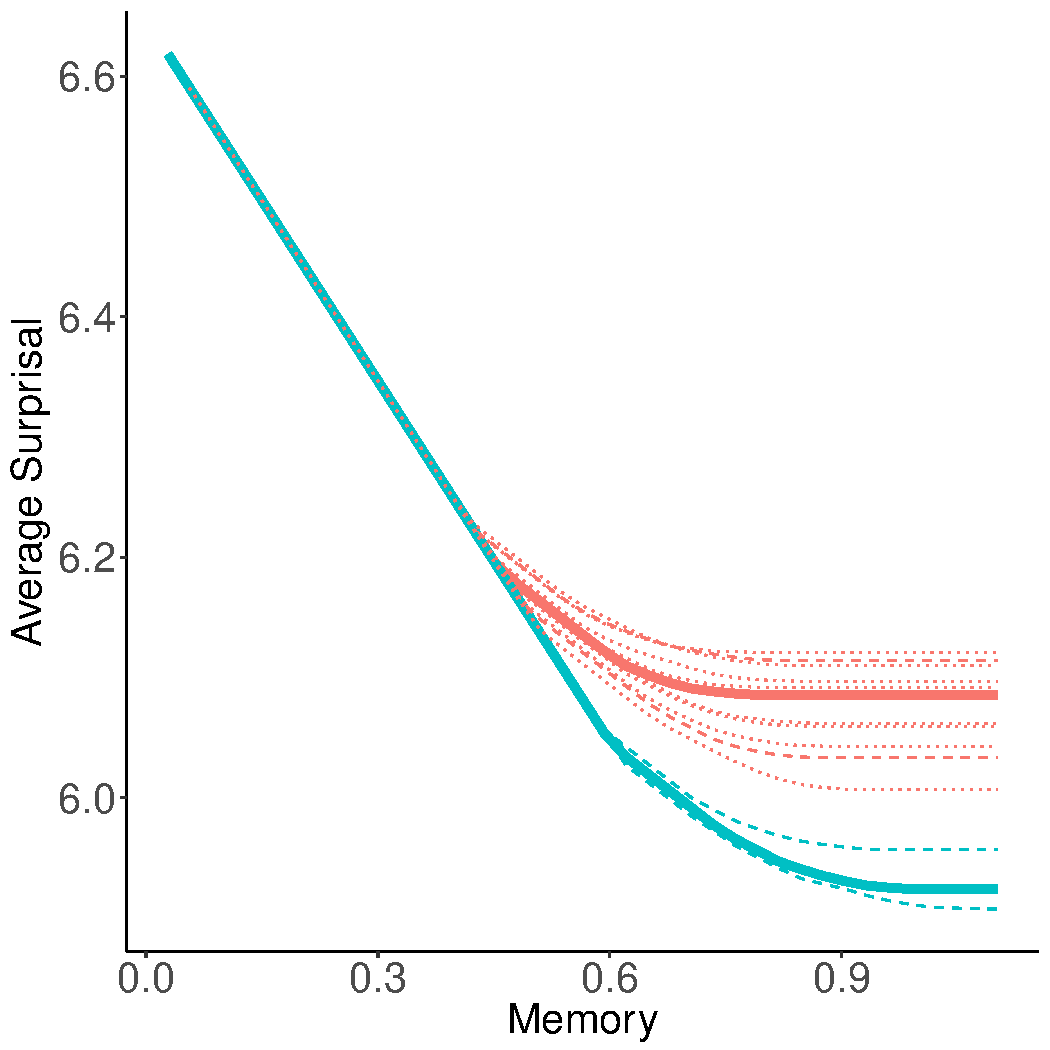
\includegraphics[width=0.25\textwidth]{neural/figures/Afrikaans-listener-surprisal-memory-MEDIANS_QUANTILES_onlyWordForms_boundedVocab_REAL.pdf} & 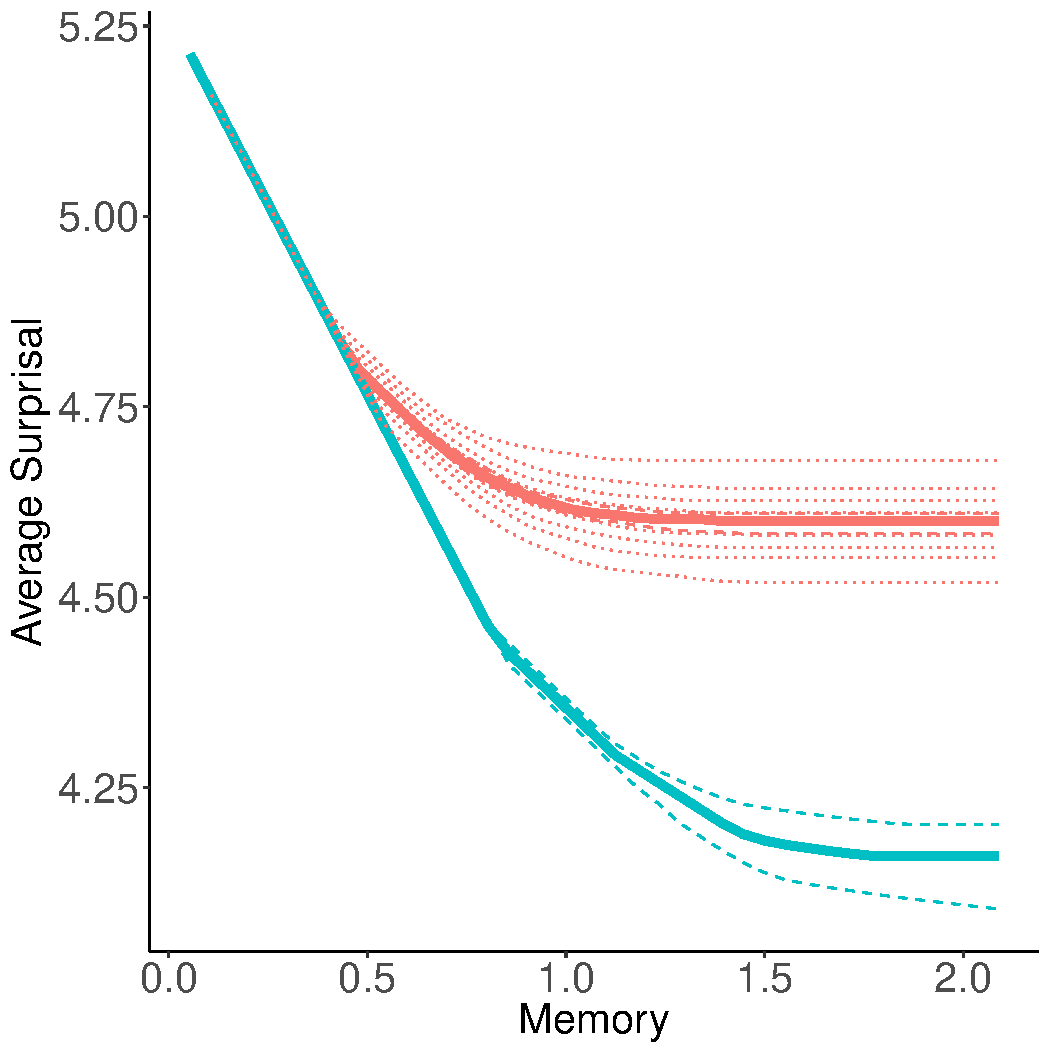
\includegraphics[width=0.25\textwidth]{neural/figures/Amharic-Adap-listener-surprisal-memory-MEDIANS_QUANTILES_onlyWordForms_boundedVocab_REAL.pdf} & 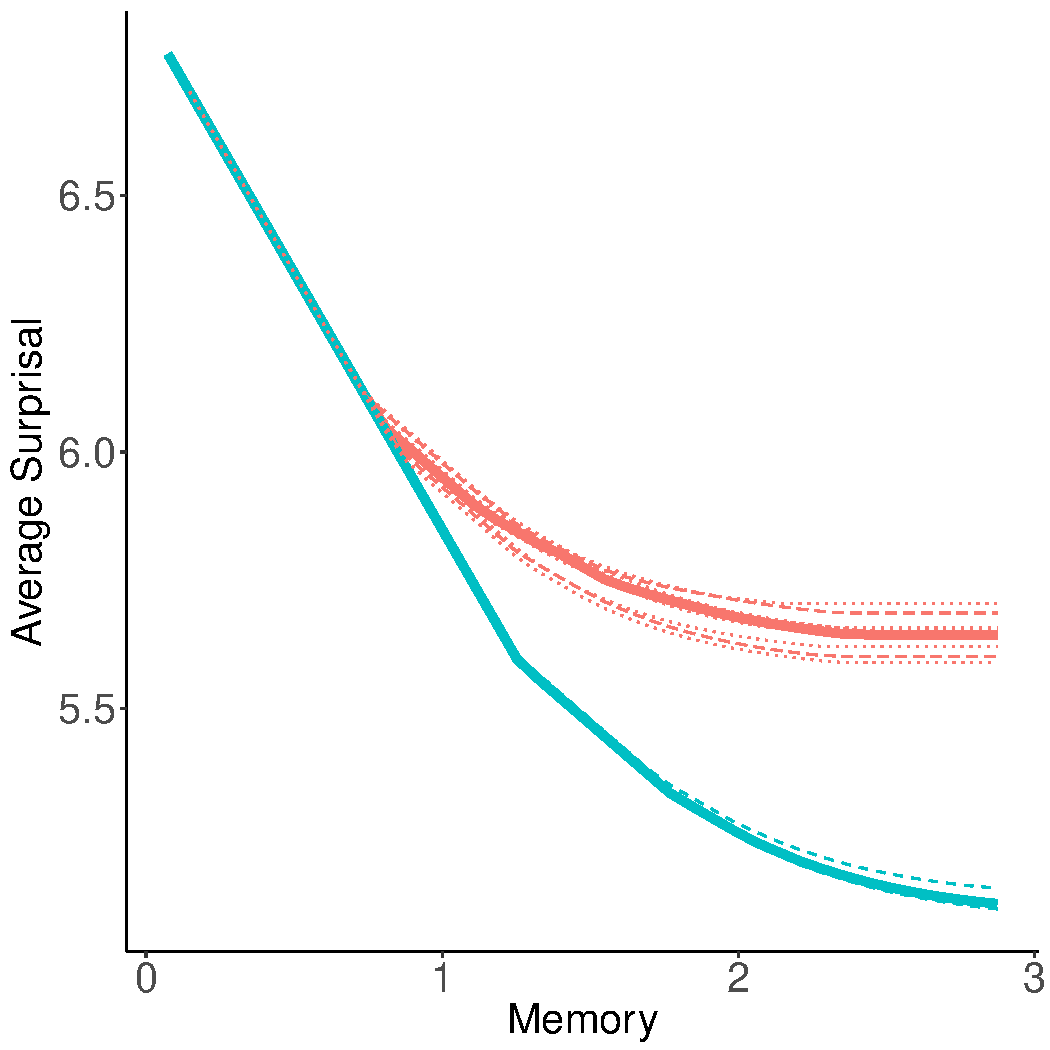
\includegraphics[width=0.25\textwidth]{neural/figures/Arabic-listener-surprisal-memory-MEDIANS_QUANTILES_onlyWordForms_boundedVocab_REAL.pdf} & 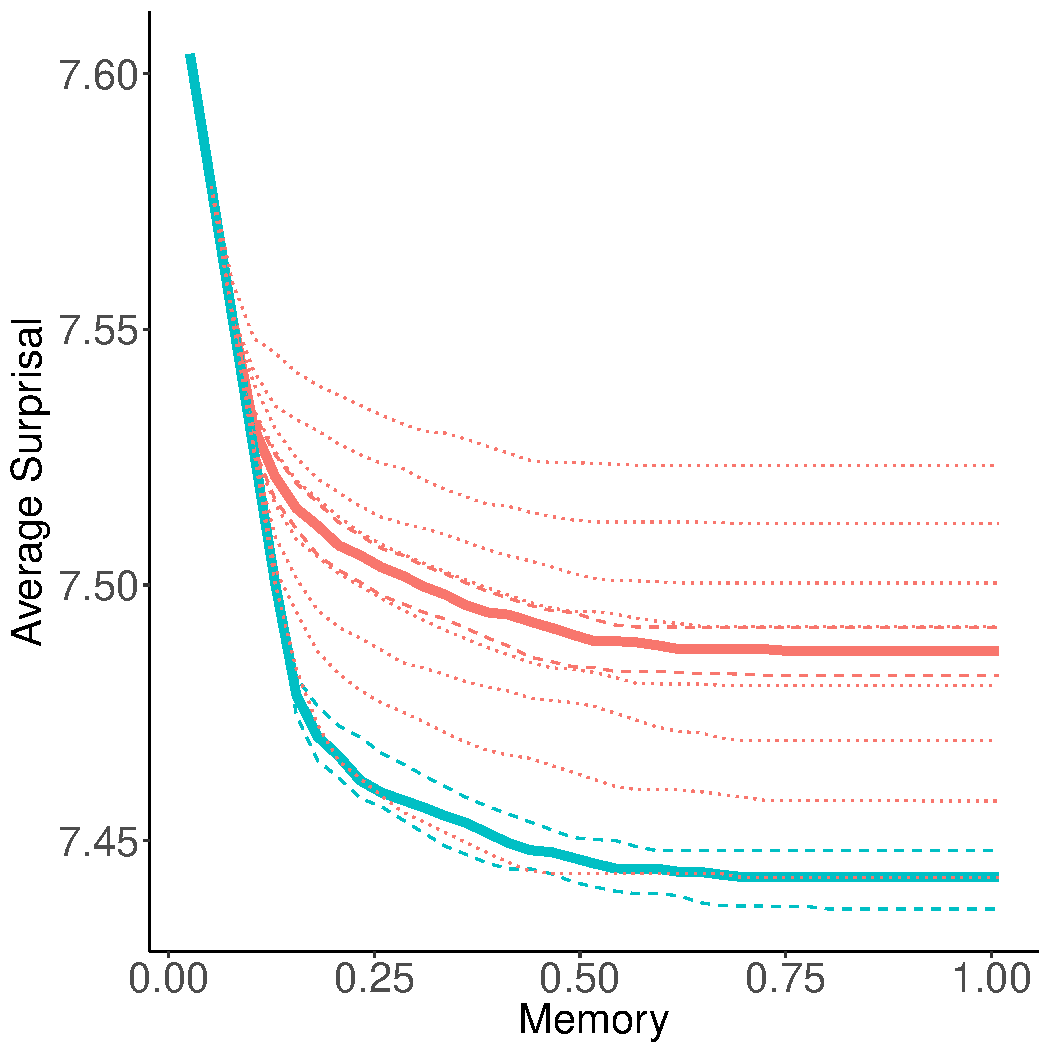
\includegraphics[width=0.25\textwidth]{neural/figures/Armenian-Adap-listener-surprisal-memory-MEDIANS_QUANTILES_onlyWordForms_boundedVocab_REAL.pdf}
 \\ 
Bambara & Basque & Breton & Bulgarian
 \\ 
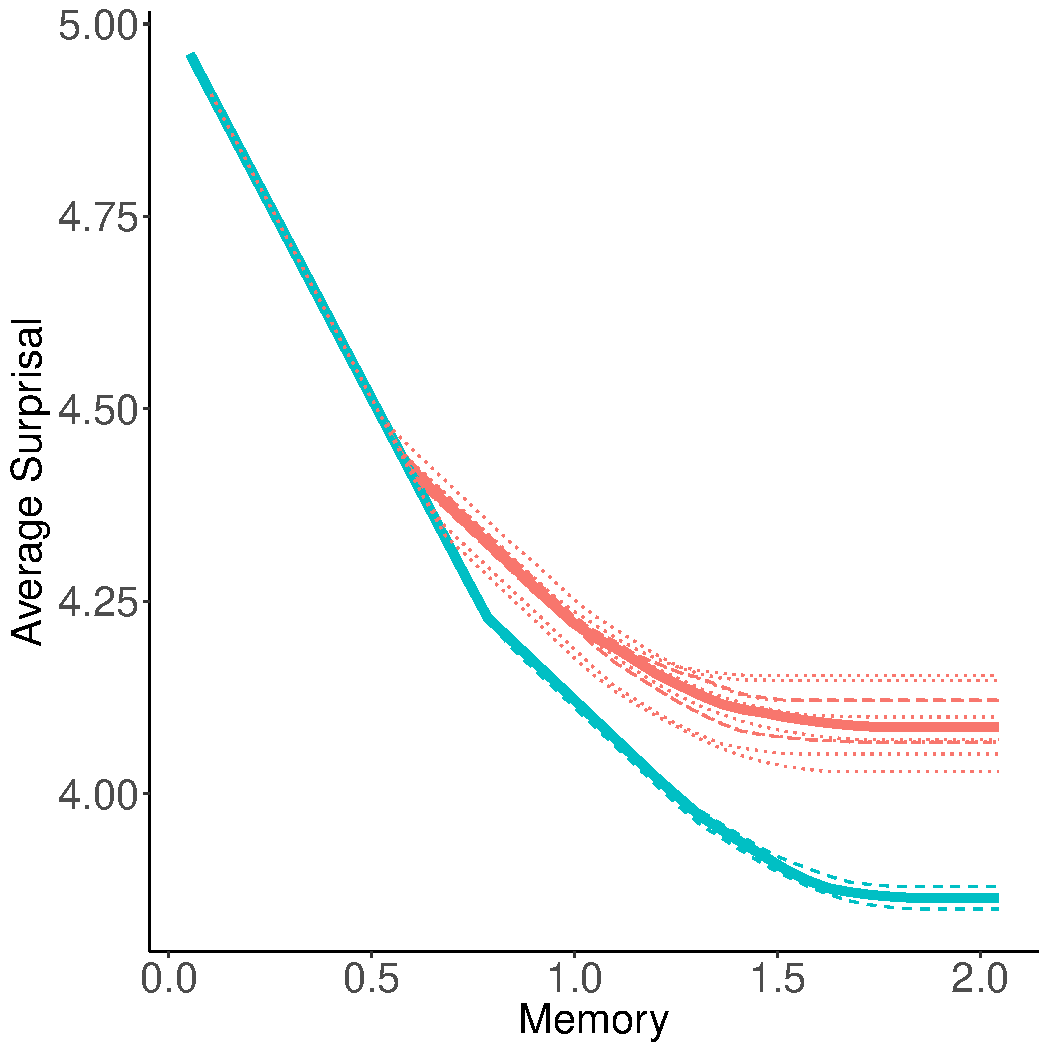
\includegraphics[width=0.25\textwidth]{neural/figures/Bambara-Adap-listener-surprisal-memory-MEDIANS_QUANTILES_onlyWordForms_boundedVocab_REAL.pdf} & 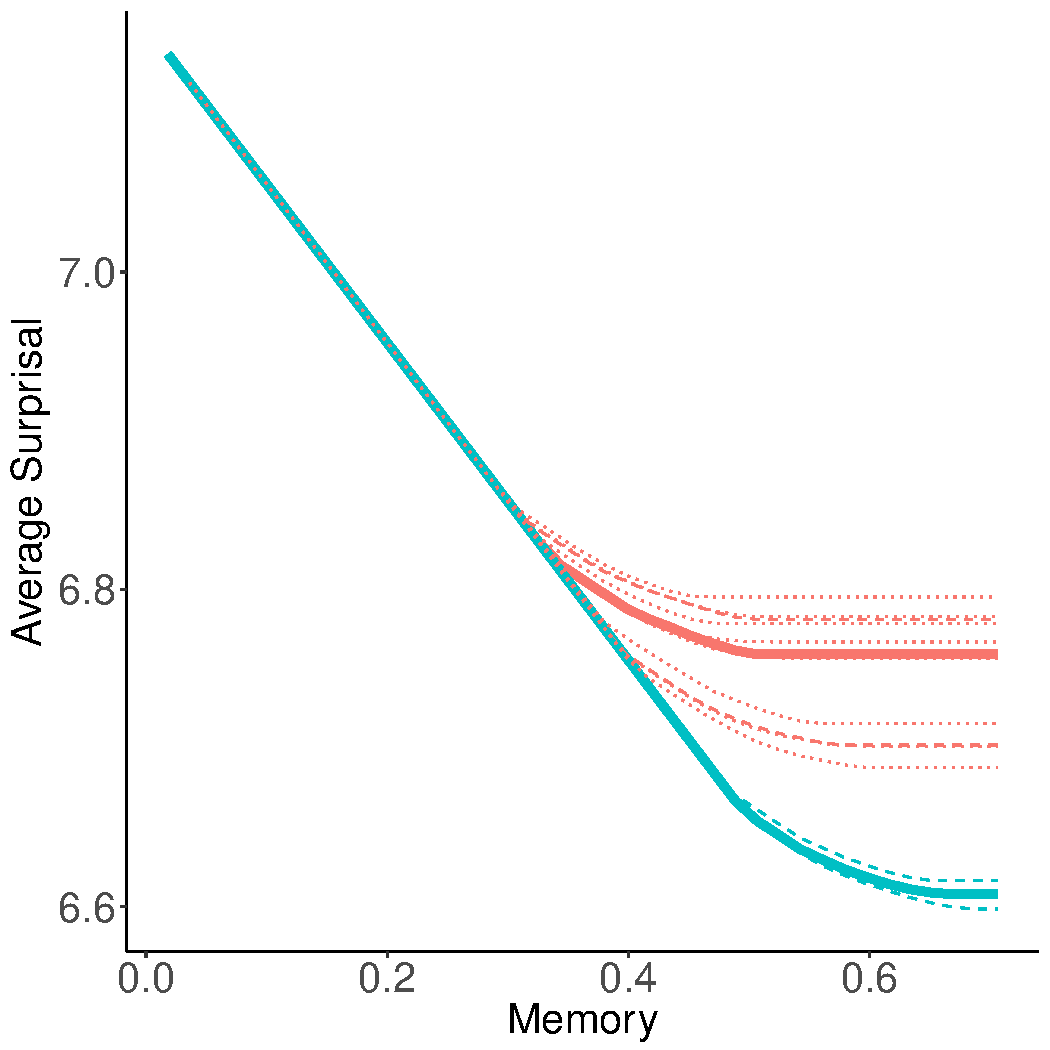
\includegraphics[width=0.25\textwidth]{neural/figures/Basque-listener-surprisal-memory-MEDIANS_QUANTILES_onlyWordForms_boundedVocab_REAL.pdf} & 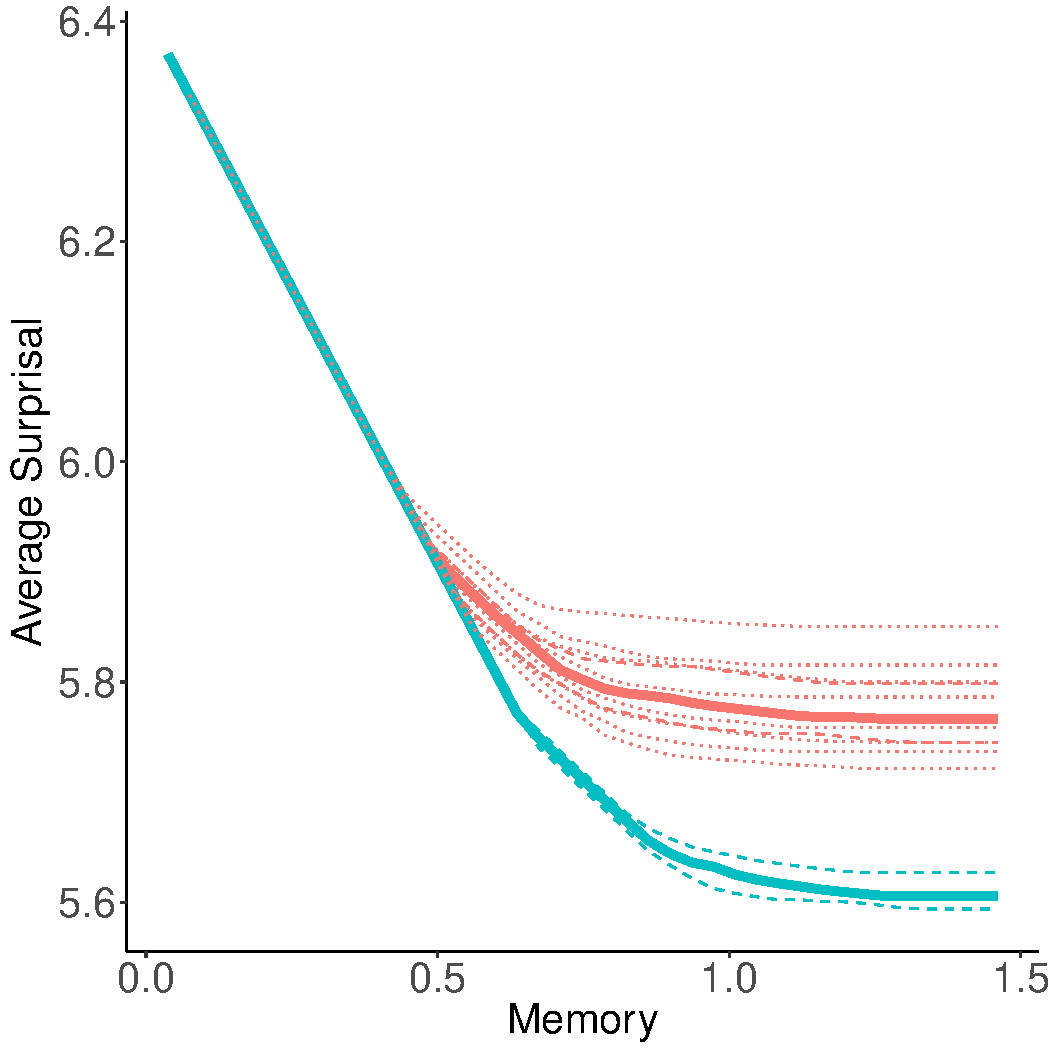
\includegraphics[width=0.25\textwidth]{neural/figures/Breton-Adap-listener-surprisal-memory-MEDIANS_QUANTILES_onlyWordForms_boundedVocab_REAL.pdf} & 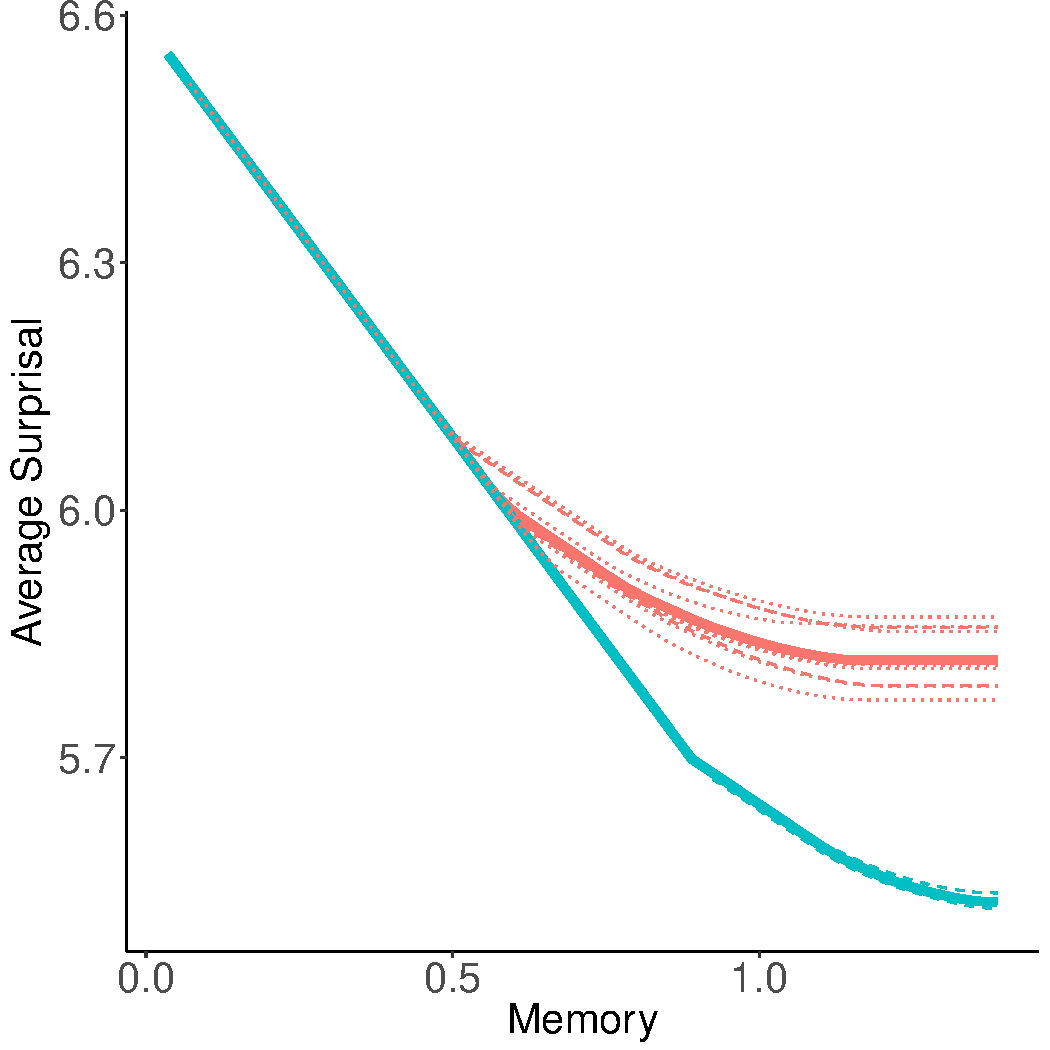
\includegraphics[width=0.25\textwidth]{neural/figures/Bulgarian-listener-surprisal-memory-MEDIANS_QUANTILES_onlyWordForms_boundedVocab_REAL.pdf}
 \\ 
Buryat & Cantonese & Catalan & Chinese
 \\ 
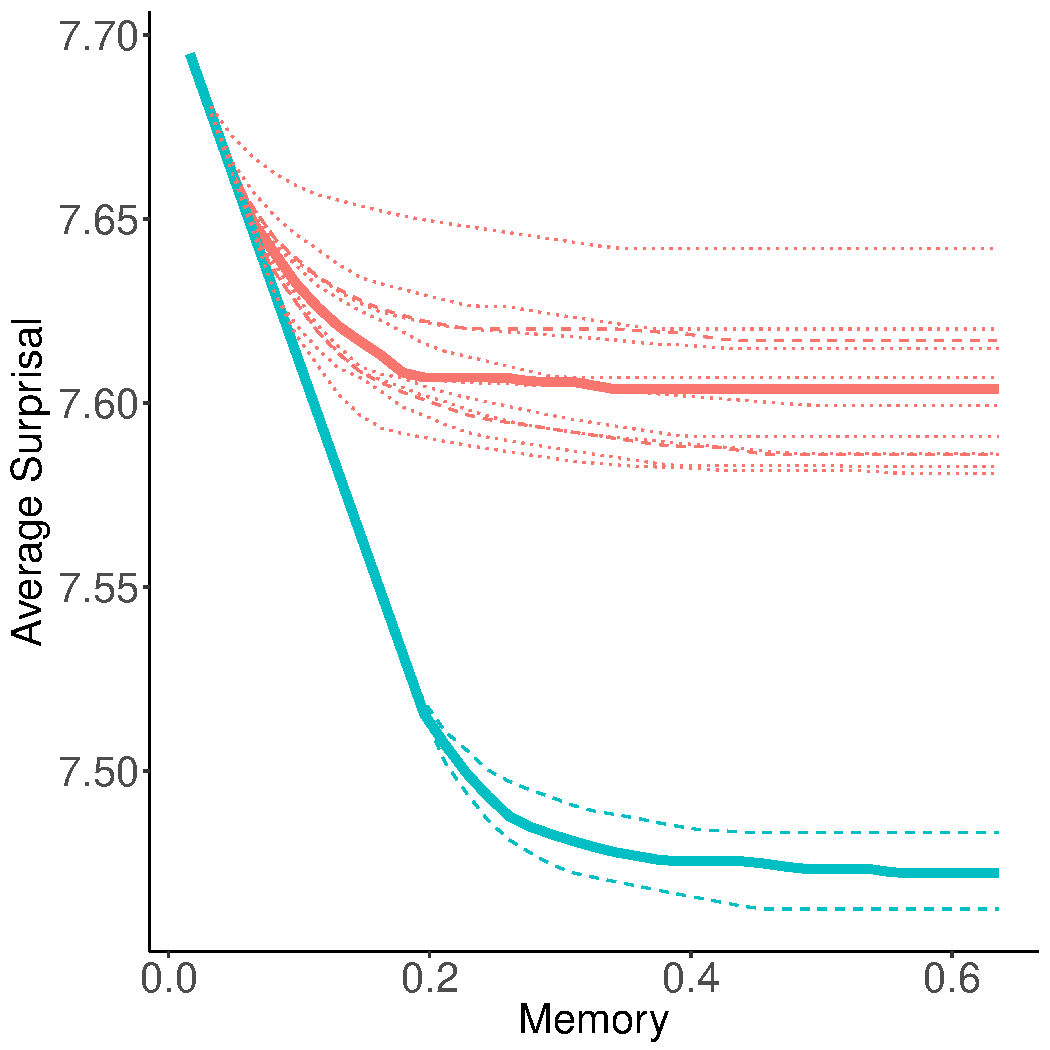
\includegraphics[width=0.25\textwidth]{neural/figures/Buryat-Adap-listener-surprisal-memory-MEDIANS_QUANTILES_onlyWordForms_boundedVocab_REAL.pdf} & 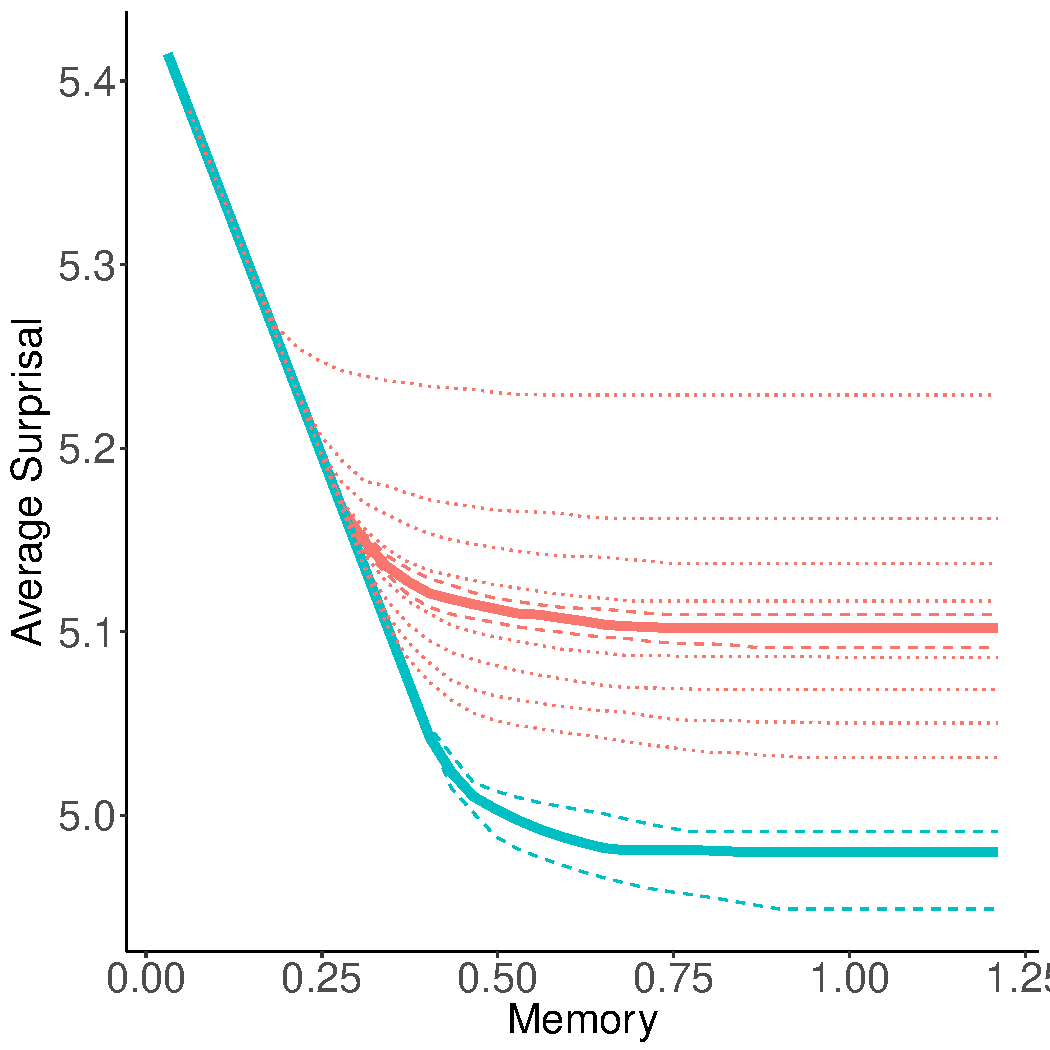
\includegraphics[width=0.25\textwidth]{neural/figures/Cantonese-Adap-listener-surprisal-memory-MEDIANS_QUANTILES_onlyWordForms_boundedVocab_REAL.pdf} & 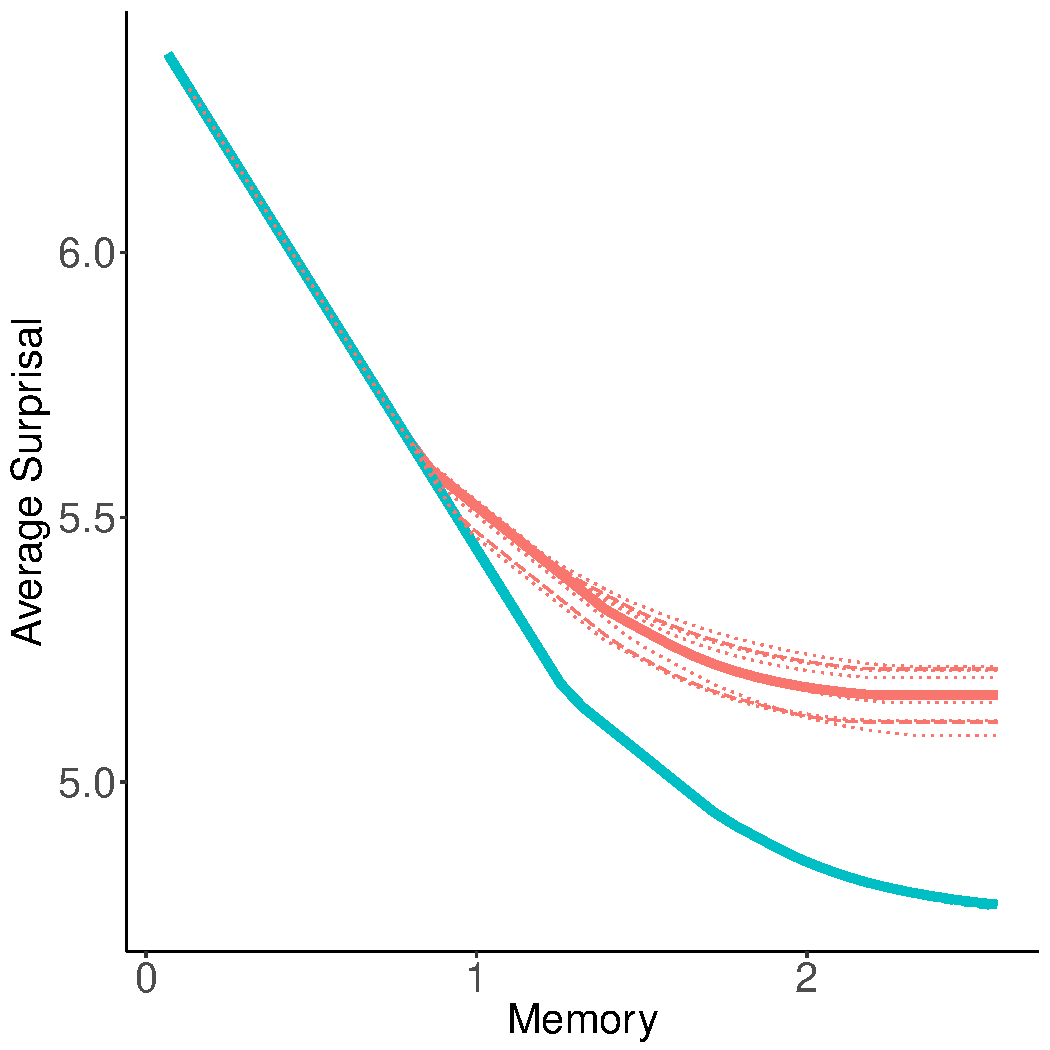
\includegraphics[width=0.25\textwidth]{neural/figures/Catalan-listener-surprisal-memory-MEDIANS_QUANTILES_onlyWordForms_boundedVocab_REAL.pdf} & 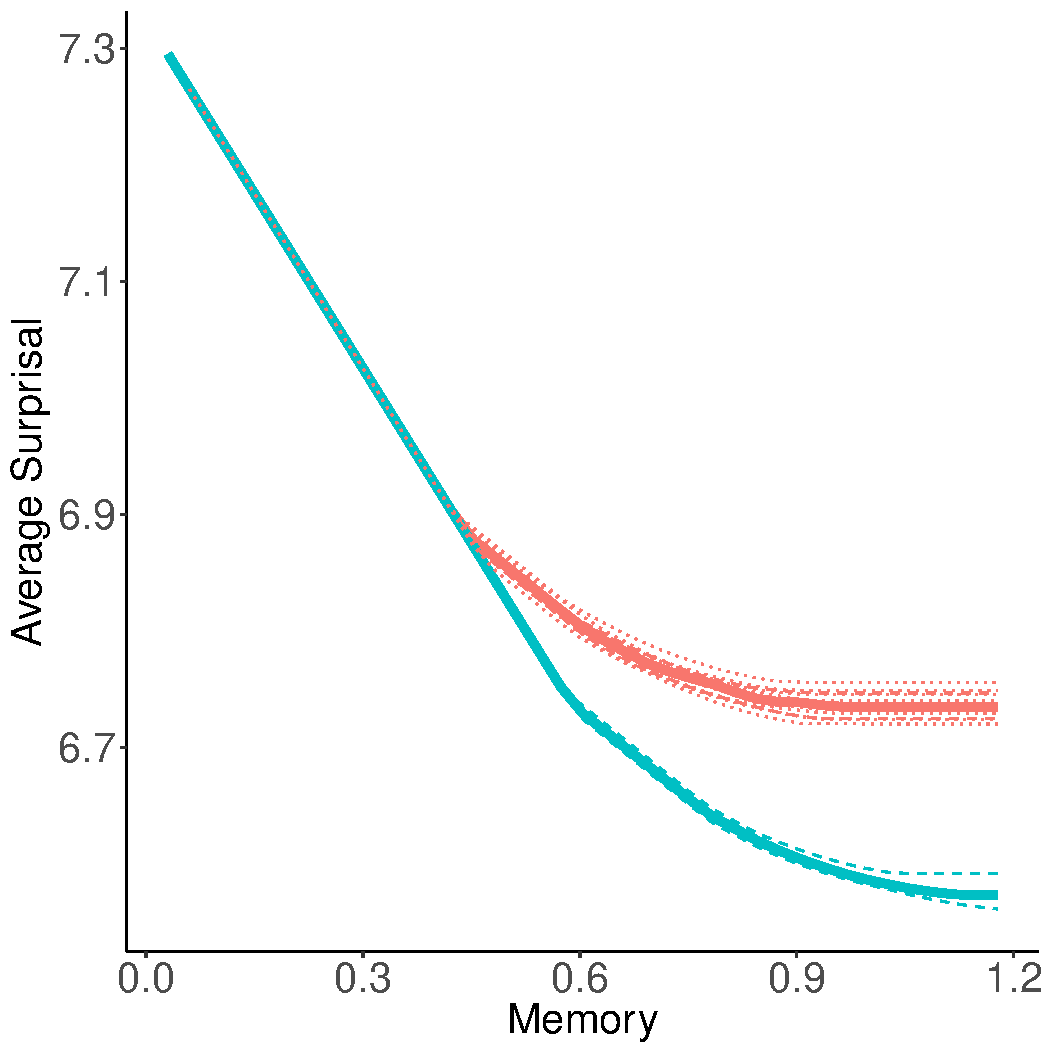
\includegraphics[width=0.25\textwidth]{neural/figures/Chinese-listener-surprisal-memory-MEDIANS_QUANTILES_onlyWordForms_boundedVocab_REAL.pdf}
 \\ 
Croatian & Czech & Danish & Dutch
 \\ 
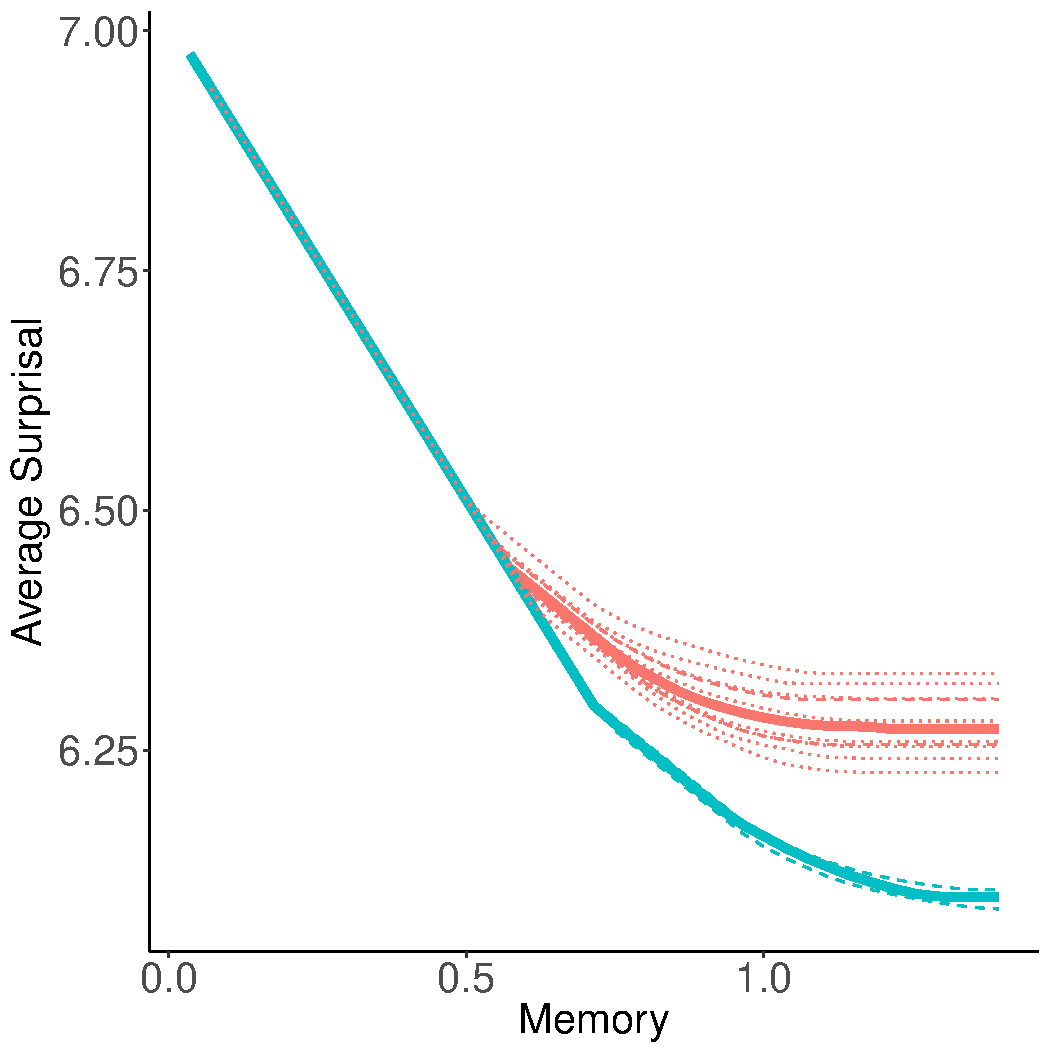
\includegraphics[width=0.25\textwidth]{neural/figures/Croatian-listener-surprisal-memory-MEDIANS_QUANTILES_onlyWordForms_boundedVocab_REAL.pdf} & 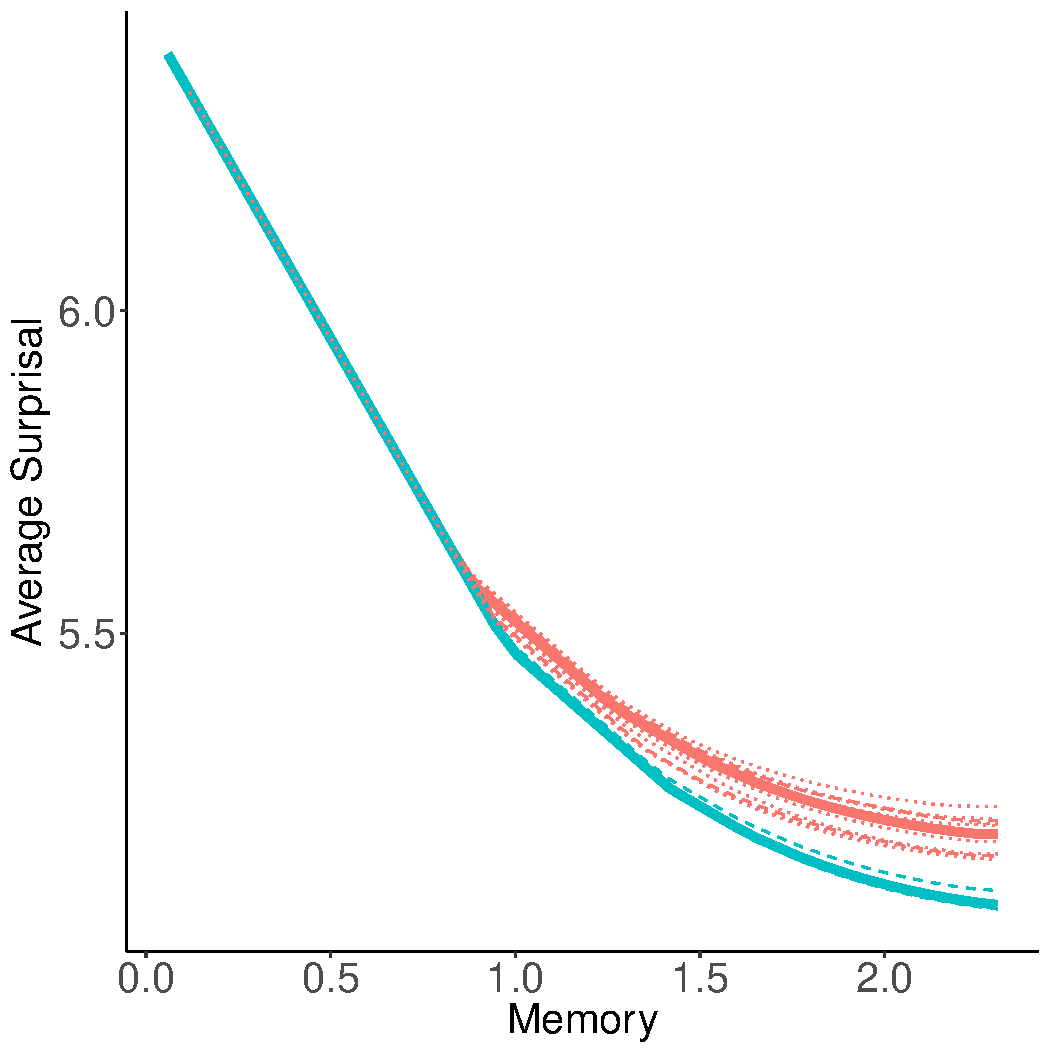
\includegraphics[width=0.25\textwidth]{neural/figures/Czech-listener-surprisal-memory-MEDIANS_QUANTILES_onlyWordForms_boundedVocab_REAL.pdf} & 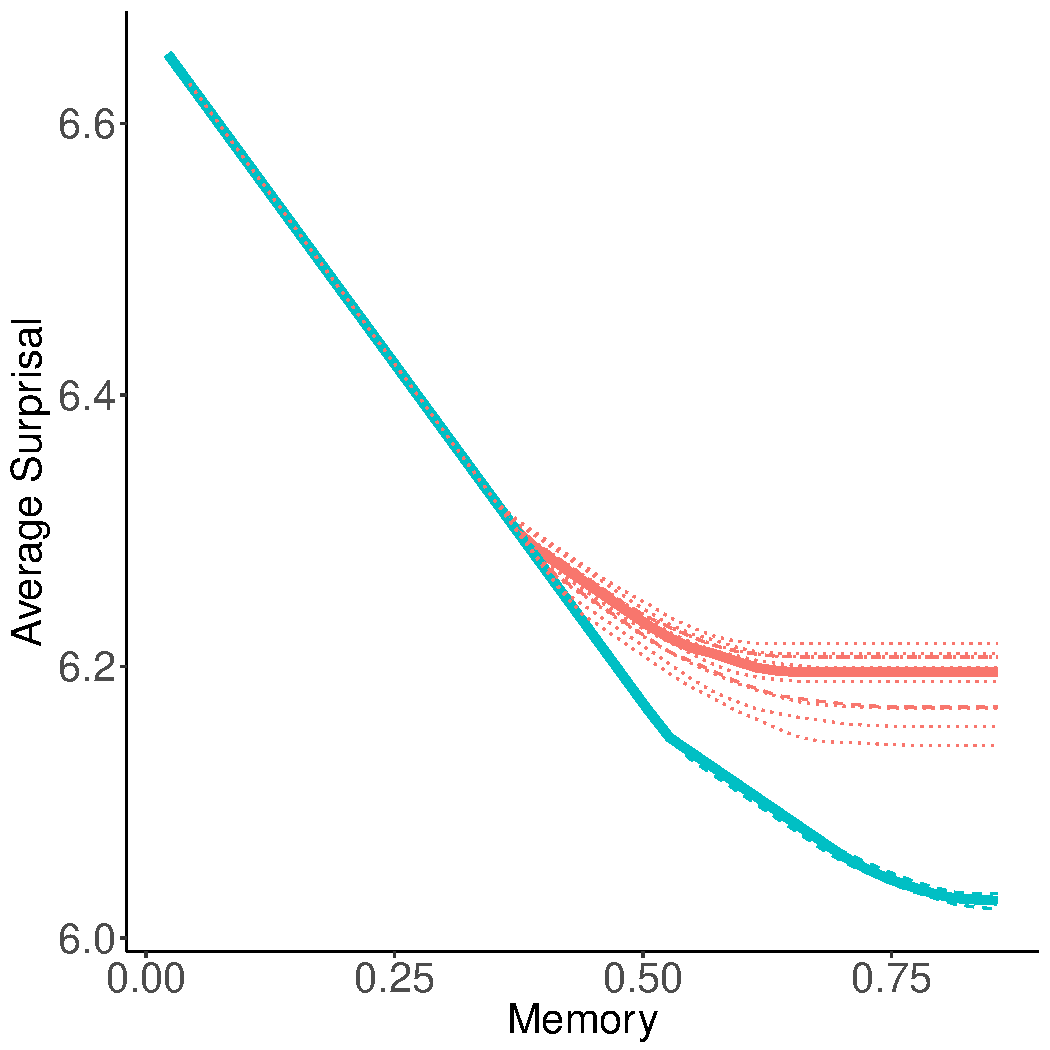
\includegraphics[width=0.25\textwidth]{neural/figures/Danish-listener-surprisal-memory-MEDIANS_QUANTILES_onlyWordForms_boundedVocab_REAL.pdf} & 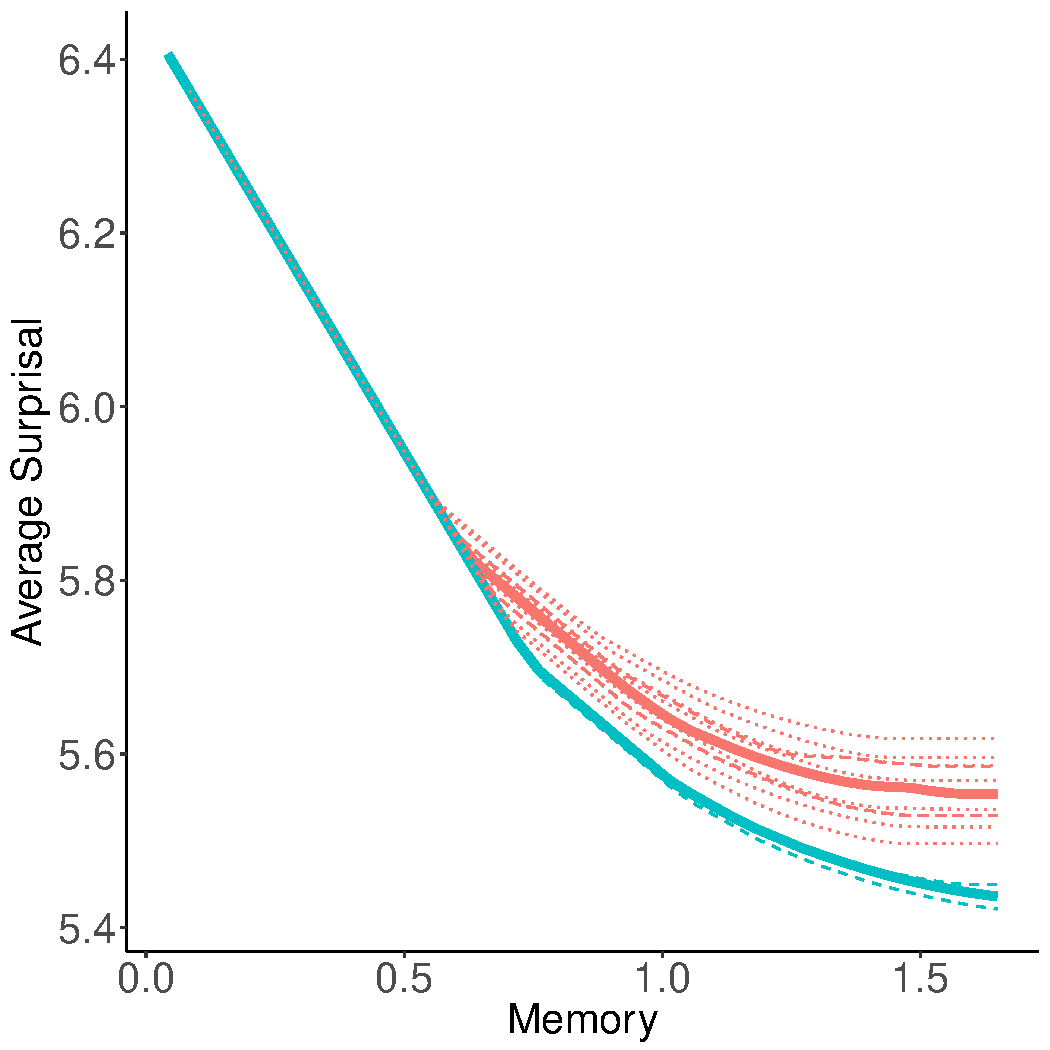
\includegraphics[width=0.25\textwidth]{neural/figures/Dutch-listener-surprisal-memory-MEDIANS_QUANTILES_onlyWordForms_boundedVocab_REAL.pdf}
 \\ 

%\end{longtable}
%	\captionof{figure}{Medians: For each memory budget, we provide the median surprisal for real and random languages. Solid lines indicate sample medians, dashed lines indicate 95 $\%$ confidence intervals for the population median, dotted lines indicate empirical quantiles ($10\%, 20\%, \dots, 80\%, 90\%$). Green: Random baselines; blue: real language; red: maximum-likelihood grammars fit to real orderings.}\label{tab:medians}
%\end{center}
%
%\begin{center}
%\begin{longtable}{ccccccccccccccclll}
%English & Erzya & Estonian & Faroese
 \\ 
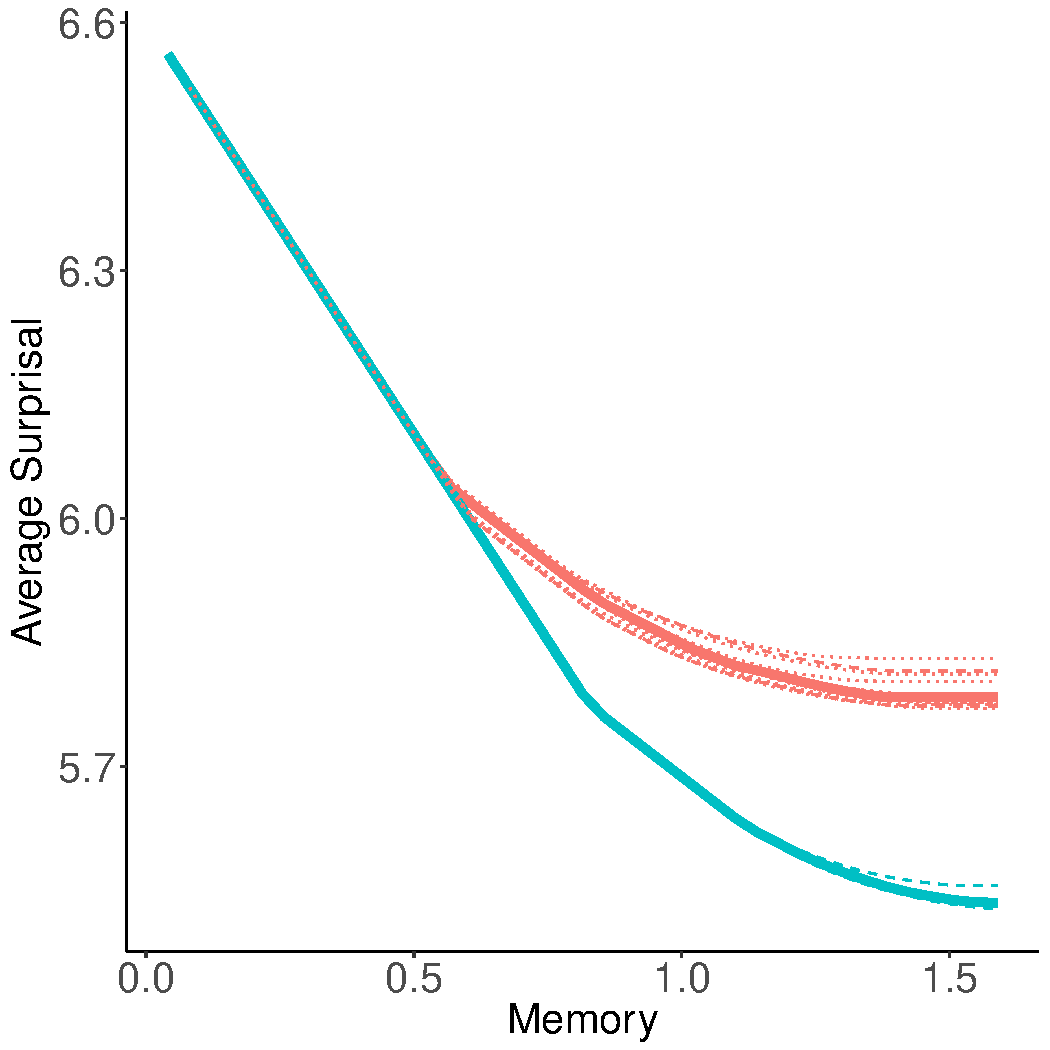
\includegraphics[width=0.25\textwidth]{neural/figures/English-listener-surprisal-memory-MEDIANS_QUANTILES_onlyWordForms_boundedVocab_REAL.pdf} & 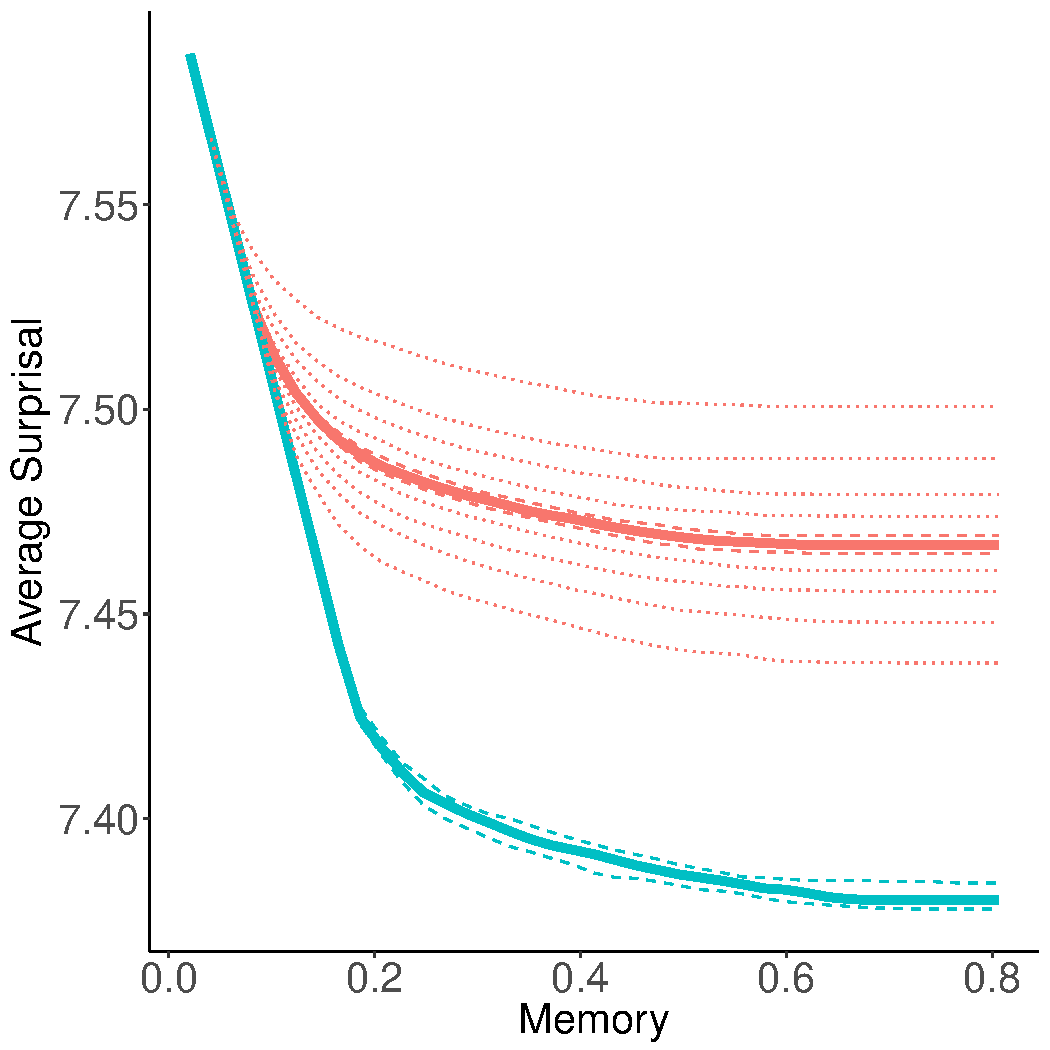
\includegraphics[width=0.25\textwidth]{neural/figures/Erzya-Adap-listener-surprisal-memory-MEDIANS_QUANTILES_onlyWordForms_boundedVocab_REAL.pdf} & 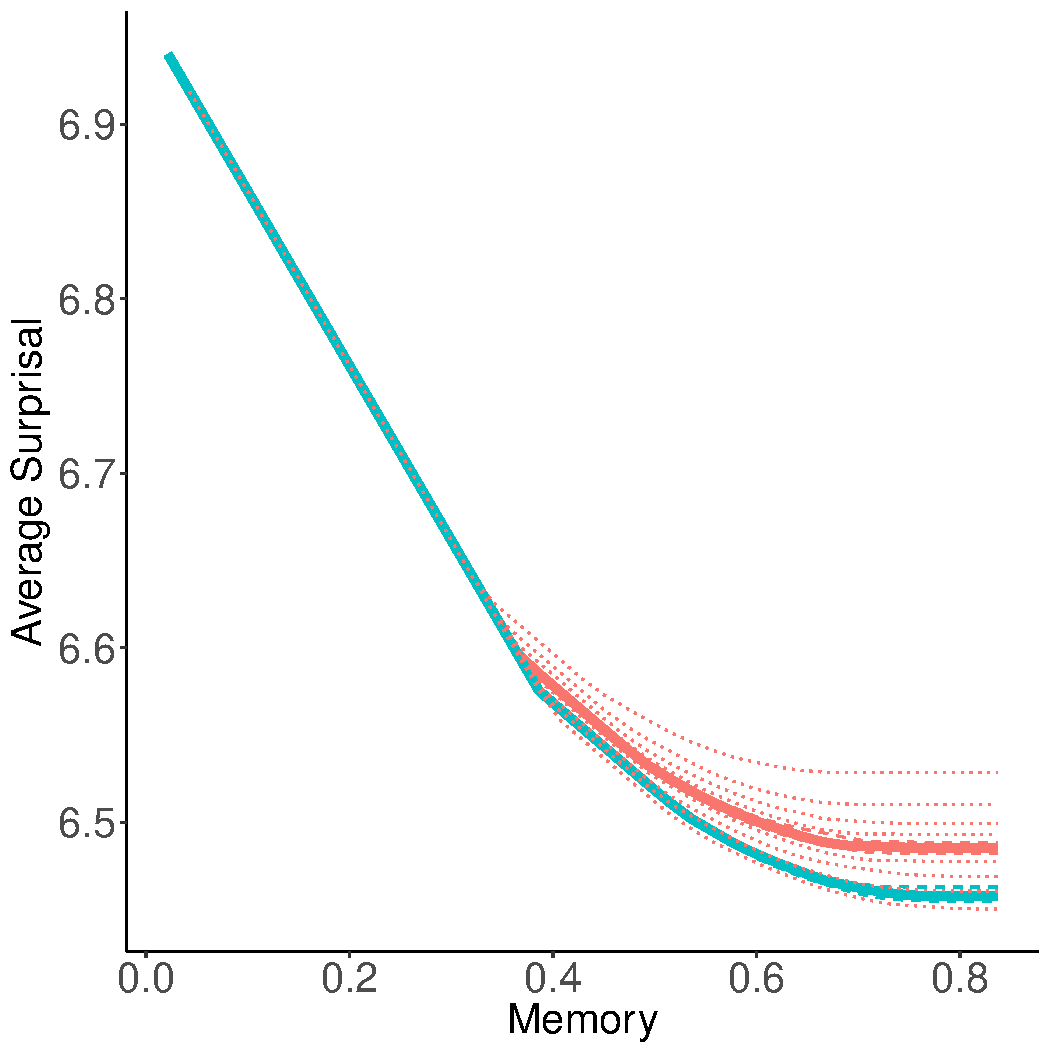
\includegraphics[width=0.25\textwidth]{neural/figures/Estonian-listener-surprisal-memory-MEDIANS_QUANTILES_onlyWordForms_boundedVocab_REAL.pdf} & 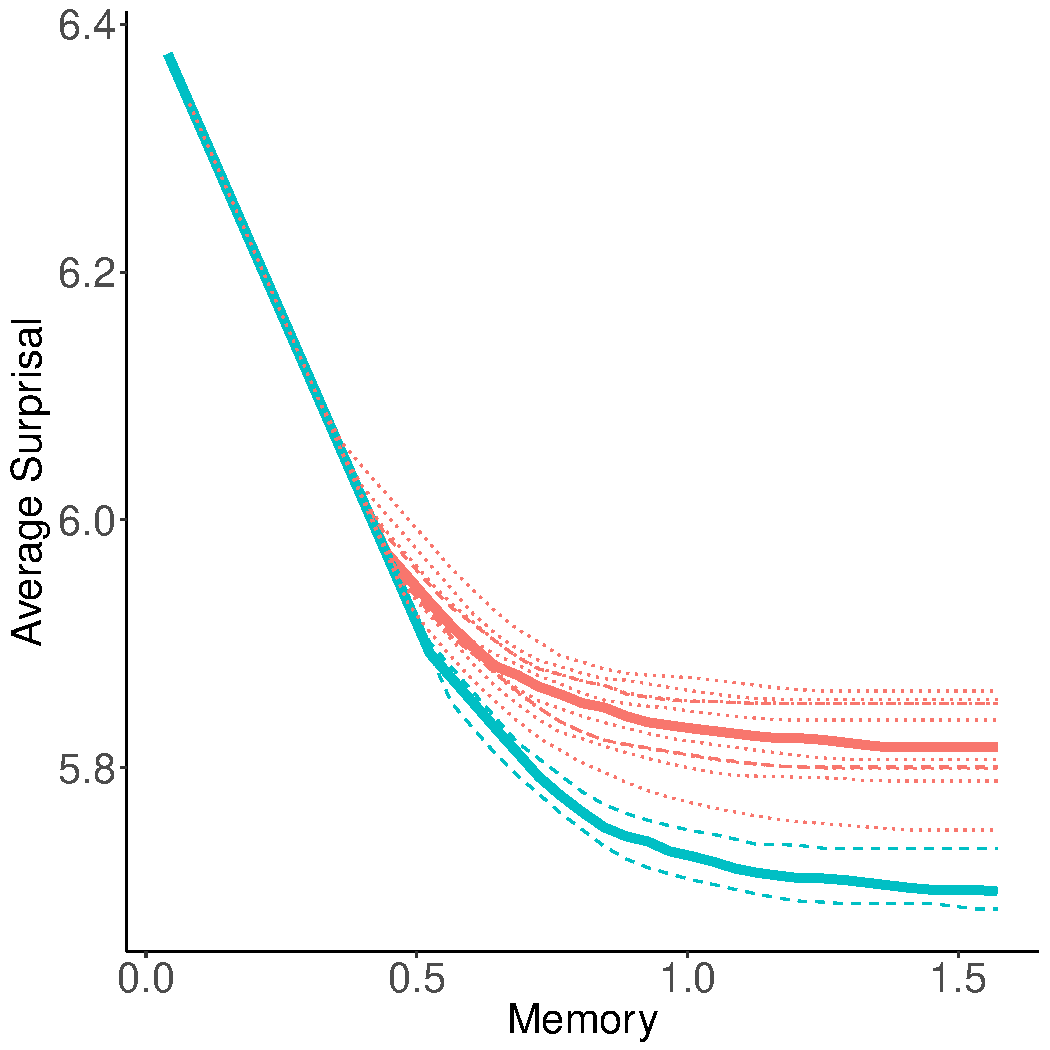
\includegraphics[width=0.25\textwidth]{neural/figures/Faroese-Adap-listener-surprisal-memory-MEDIANS_QUANTILES_onlyWordForms_boundedVocab_REAL.pdf}
 \\ 
Finnish & French & German & Greek
 \\ 
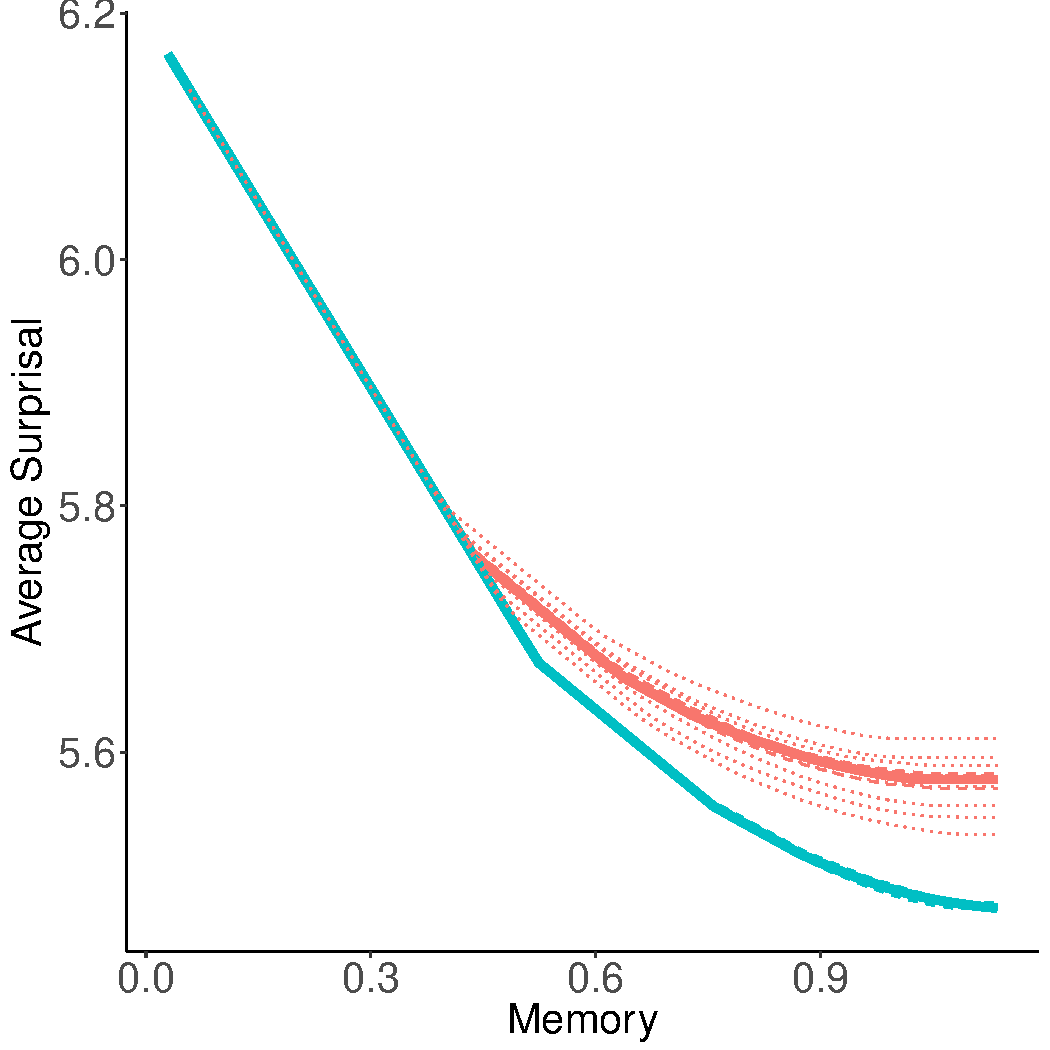
\includegraphics[width=0.25\textwidth]{neural/figures/Finnish-listener-surprisal-memory-MEDIANS_QUANTILES_onlyWordForms_boundedVocab_REAL.pdf} & 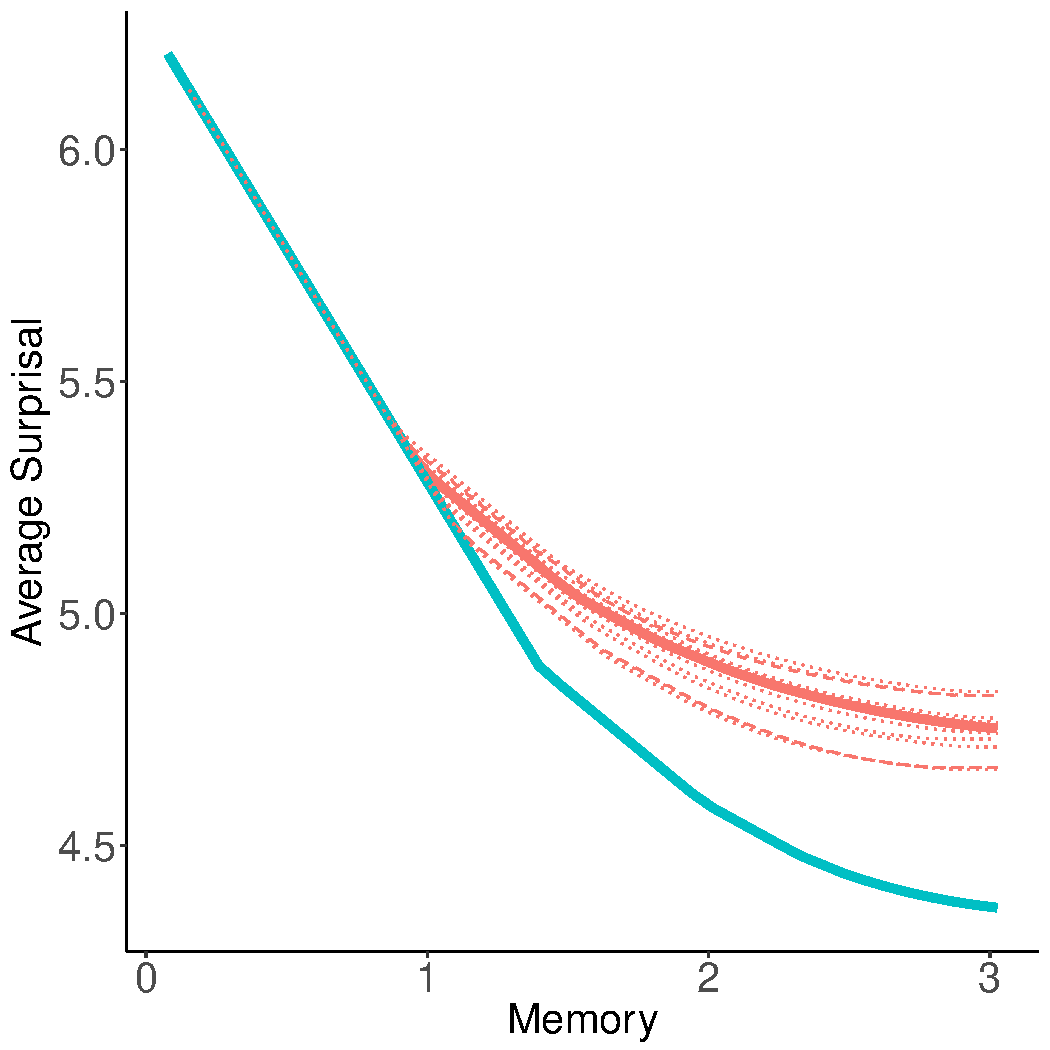
\includegraphics[width=0.25\textwidth]{neural/figures/French-listener-surprisal-memory-MEDIANS_QUANTILES_onlyWordForms_boundedVocab_REAL.pdf} & 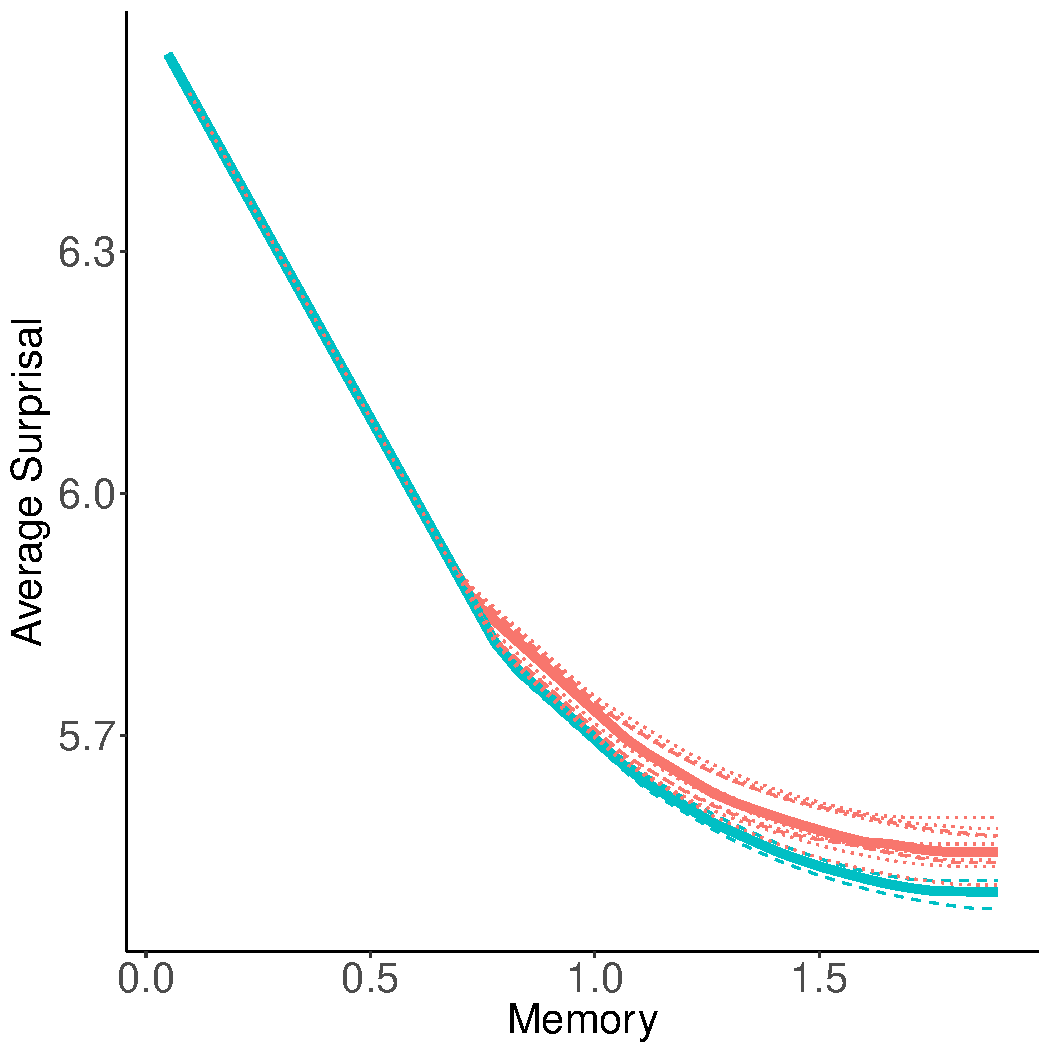
\includegraphics[width=0.25\textwidth]{neural/figures/German-listener-surprisal-memory-MEDIANS_QUANTILES_onlyWordForms_boundedVocab_REAL.pdf} & 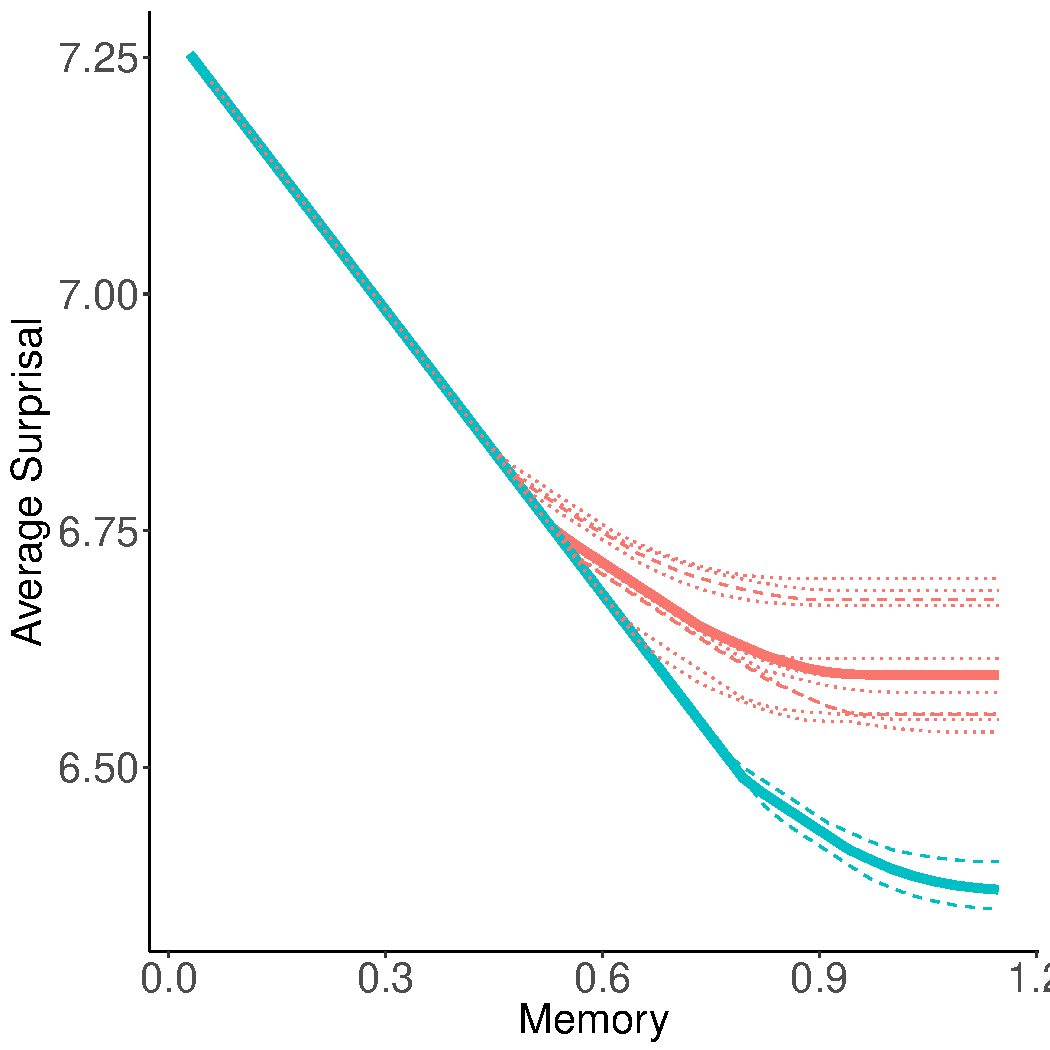
\includegraphics[width=0.25\textwidth]{neural/figures/Greek-listener-surprisal-memory-MEDIANS_QUANTILES_onlyWordForms_boundedVocab_REAL.pdf}
 \\ 
Hebrew & Hindi & Hungarian & Indonesian
 \\ 
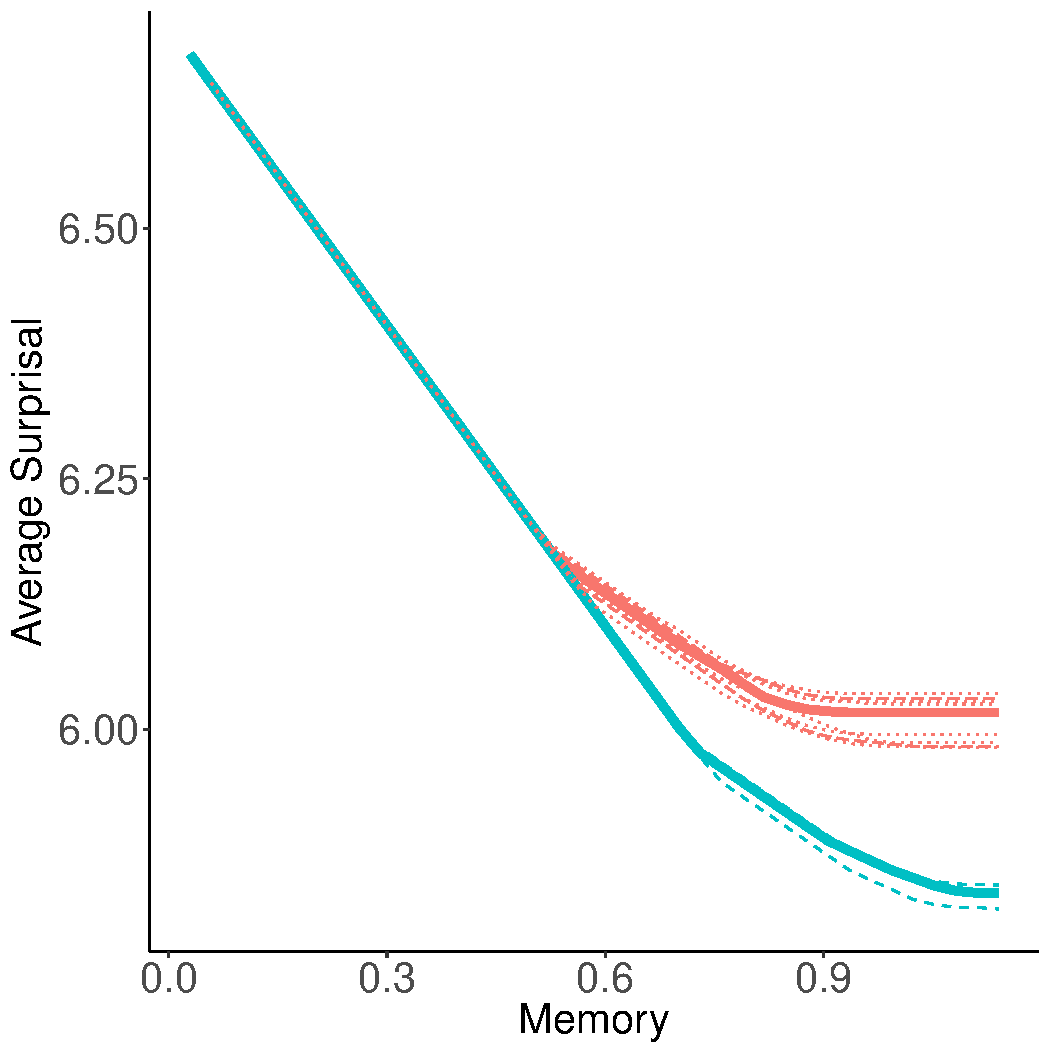
\includegraphics[width=0.25\textwidth]{neural/figures/Hebrew-listener-surprisal-memory-MEDIANS_QUANTILES_onlyWordForms_boundedVocab_REAL.pdf} & 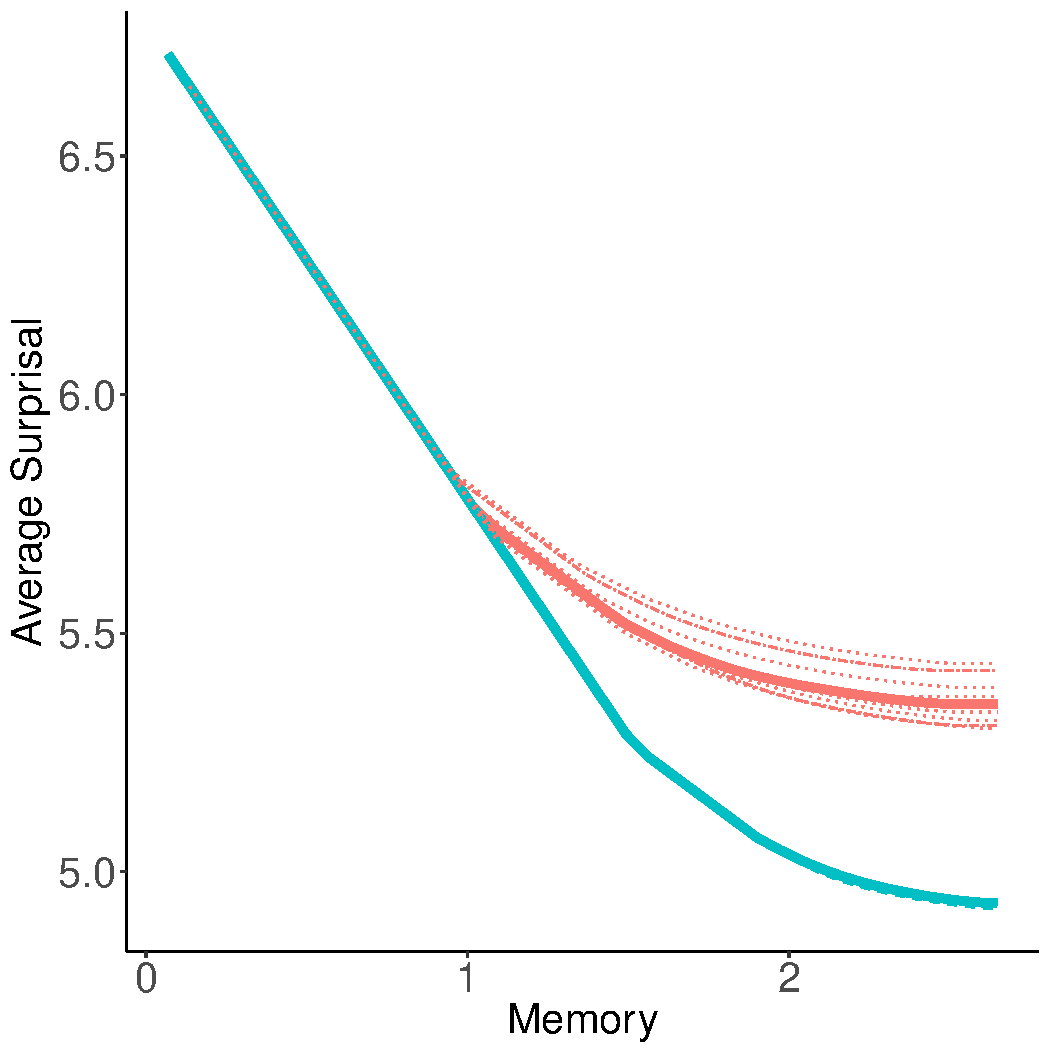
\includegraphics[width=0.25\textwidth]{neural/figures/Hindi-listener-surprisal-memory-MEDIANS_QUANTILES_onlyWordForms_boundedVocab_REAL.pdf} & 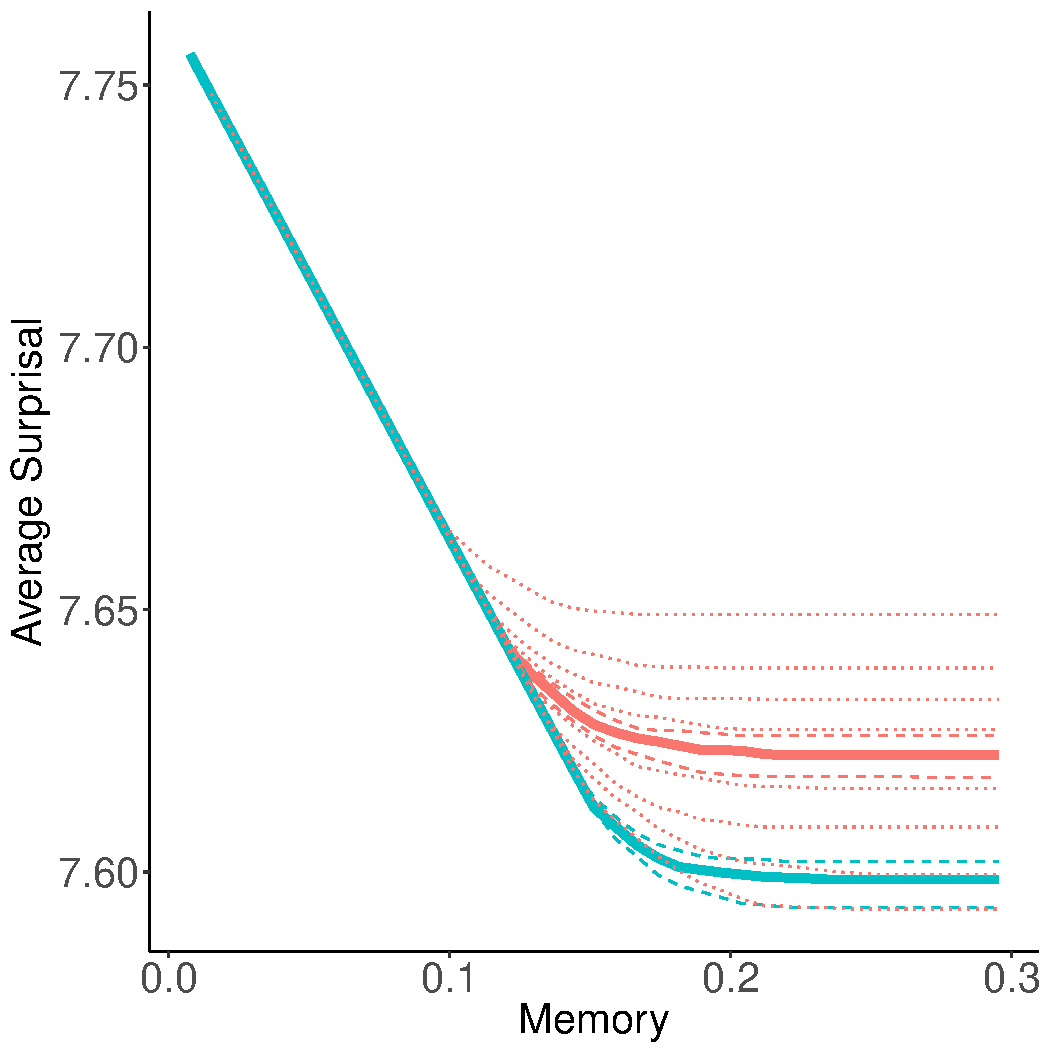
\includegraphics[width=0.25\textwidth]{neural/figures/Hungarian-listener-surprisal-memory-MEDIANS_QUANTILES_onlyWordForms_boundedVocab_REAL.pdf} & 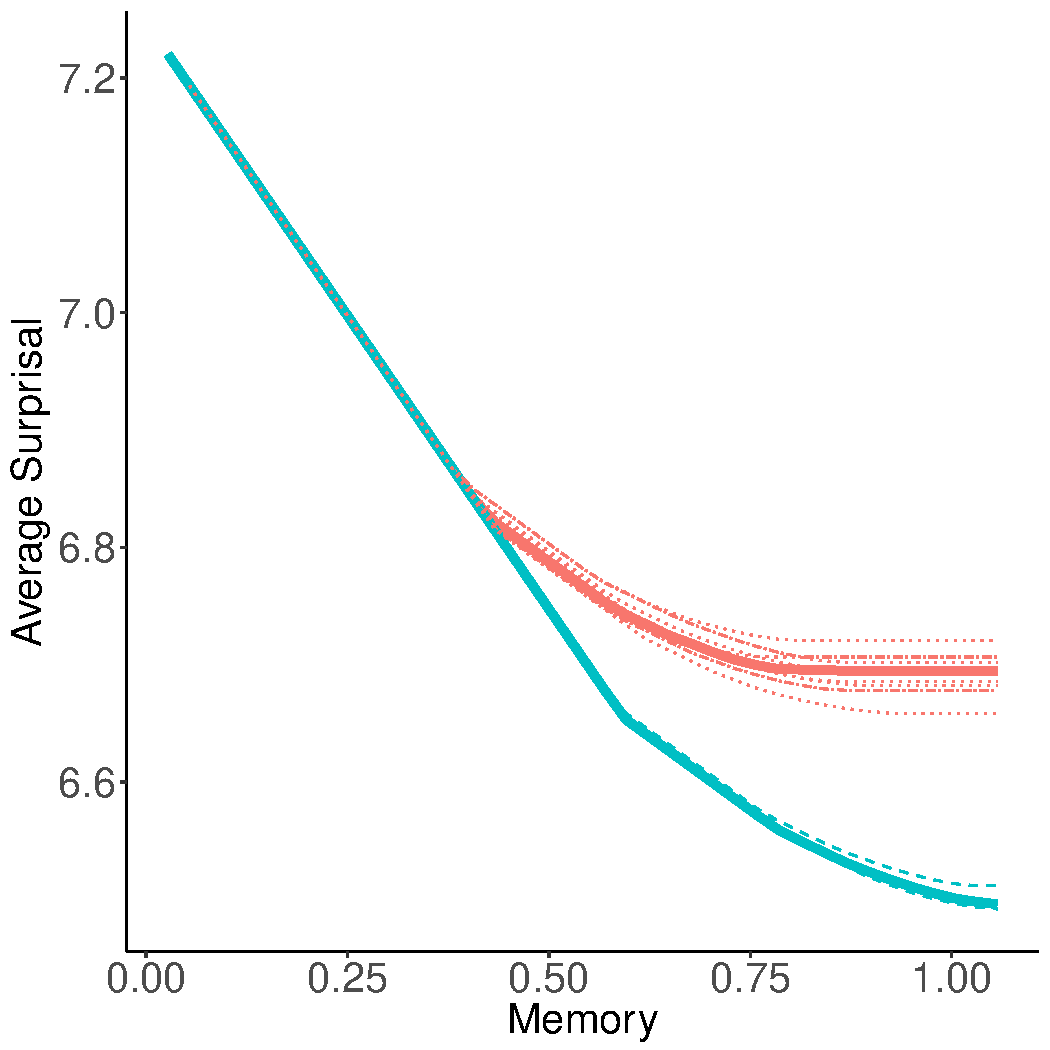
\includegraphics[width=0.25\textwidth]{neural/figures/Indonesian-listener-surprisal-memory-MEDIANS_QUANTILES_onlyWordForms_boundedVocab_REAL.pdf}
 \\ 
Italian & Japanese & Kazakh & Korean
 \\ 
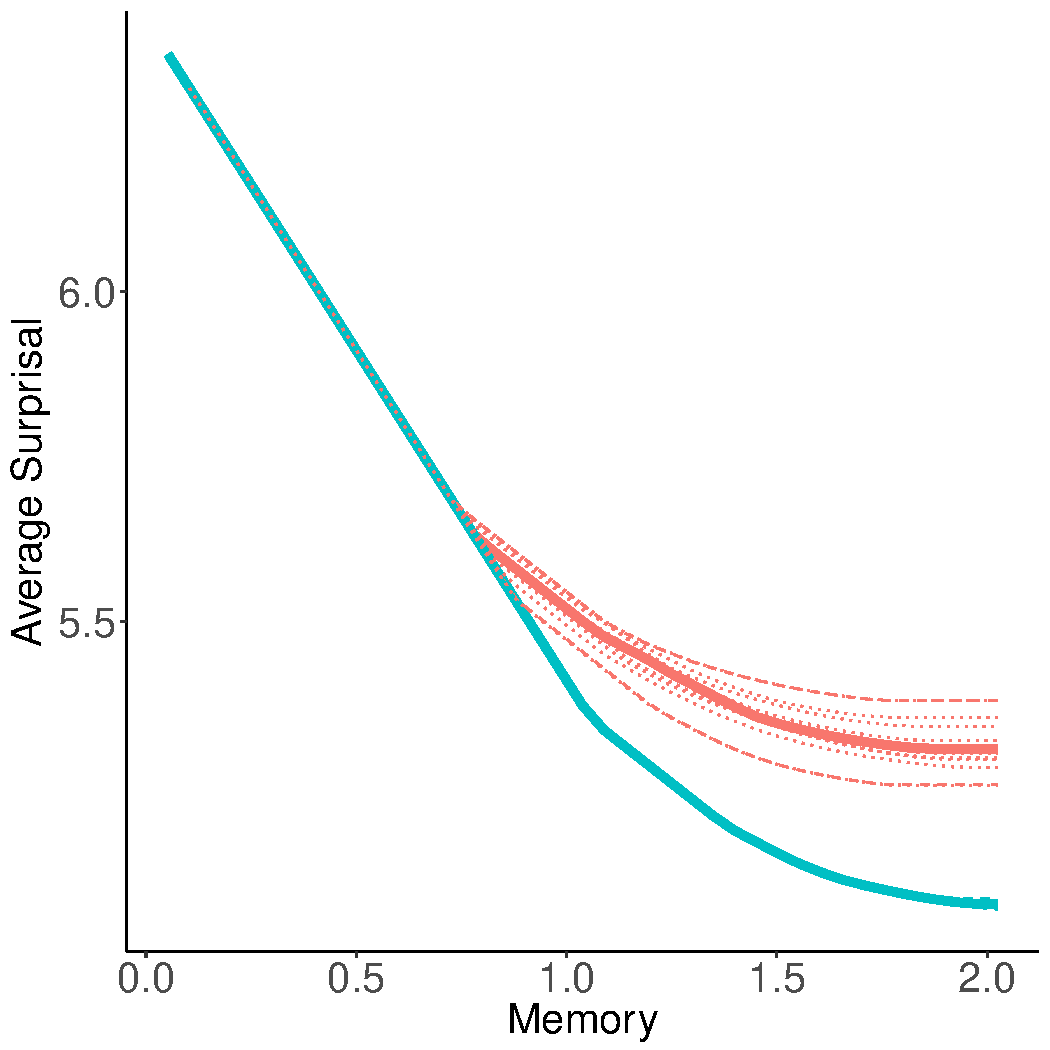
\includegraphics[width=0.25\textwidth]{neural/figures/Italian-listener-surprisal-memory-MEDIANS_QUANTILES_onlyWordForms_boundedVocab_REAL.pdf} & 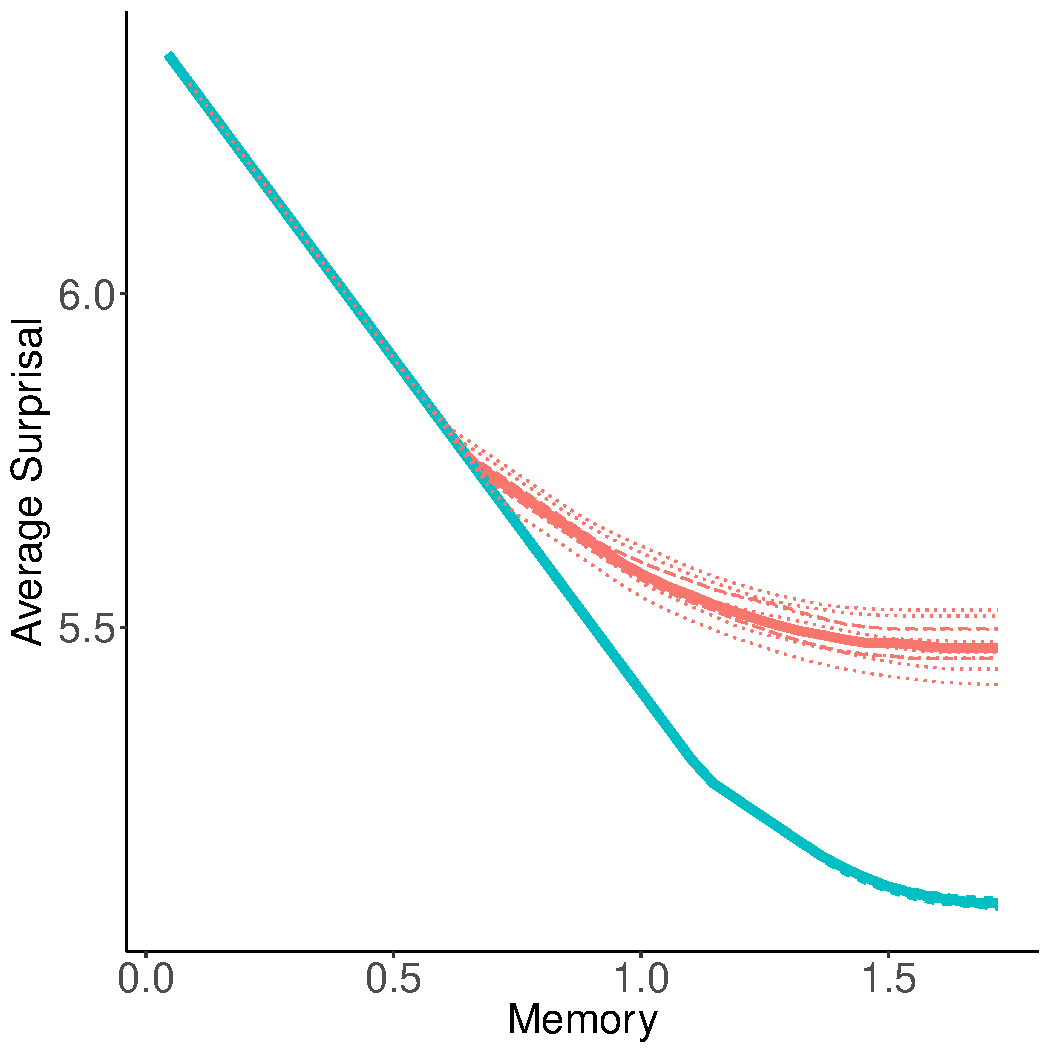
\includegraphics[width=0.25\textwidth]{neural/figures/Japanese-listener-surprisal-memory-MEDIANS_QUANTILES_onlyWordForms_boundedVocab_REAL.pdf} & 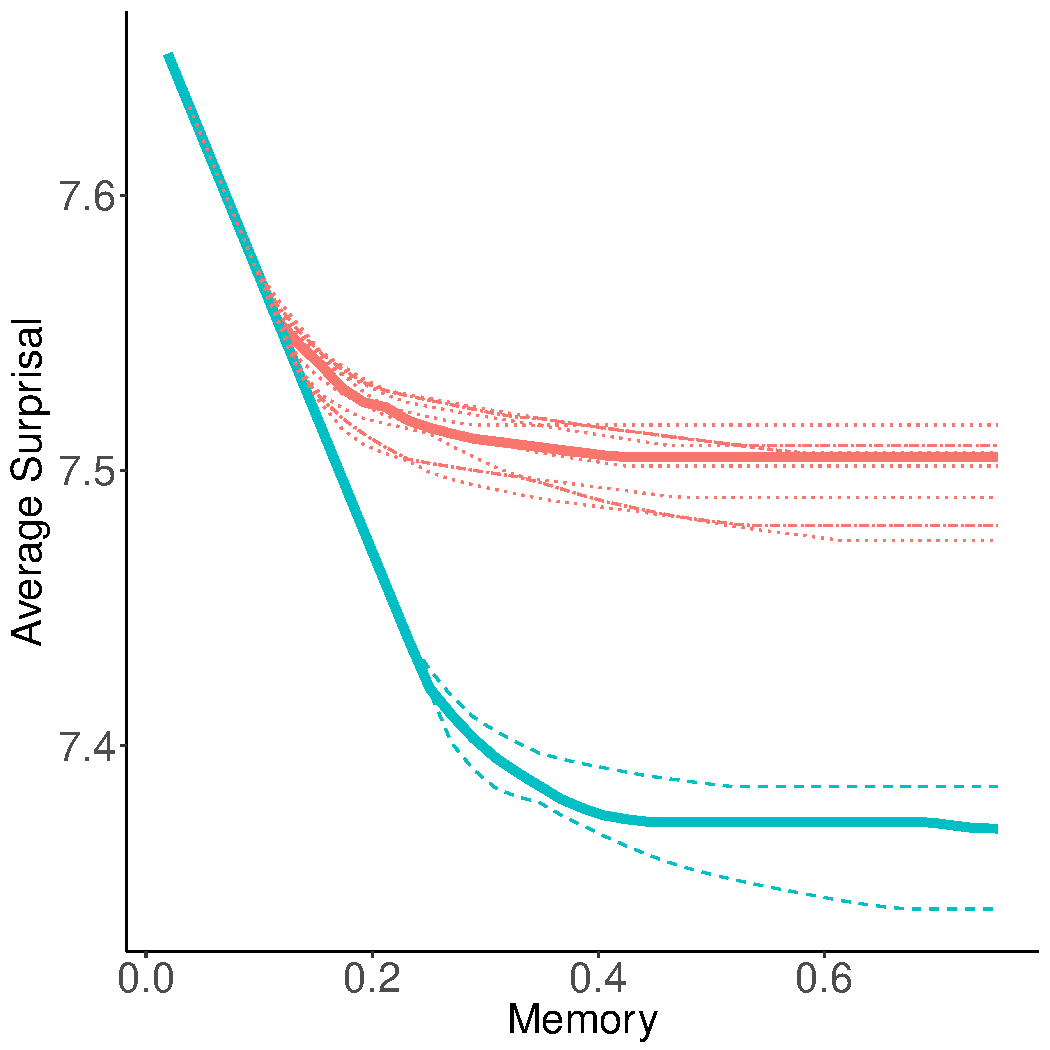
\includegraphics[width=0.25\textwidth]{neural/figures/Kazakh-Adap-listener-surprisal-memory-MEDIANS_QUANTILES_onlyWordForms_boundedVocab_REAL.pdf} & 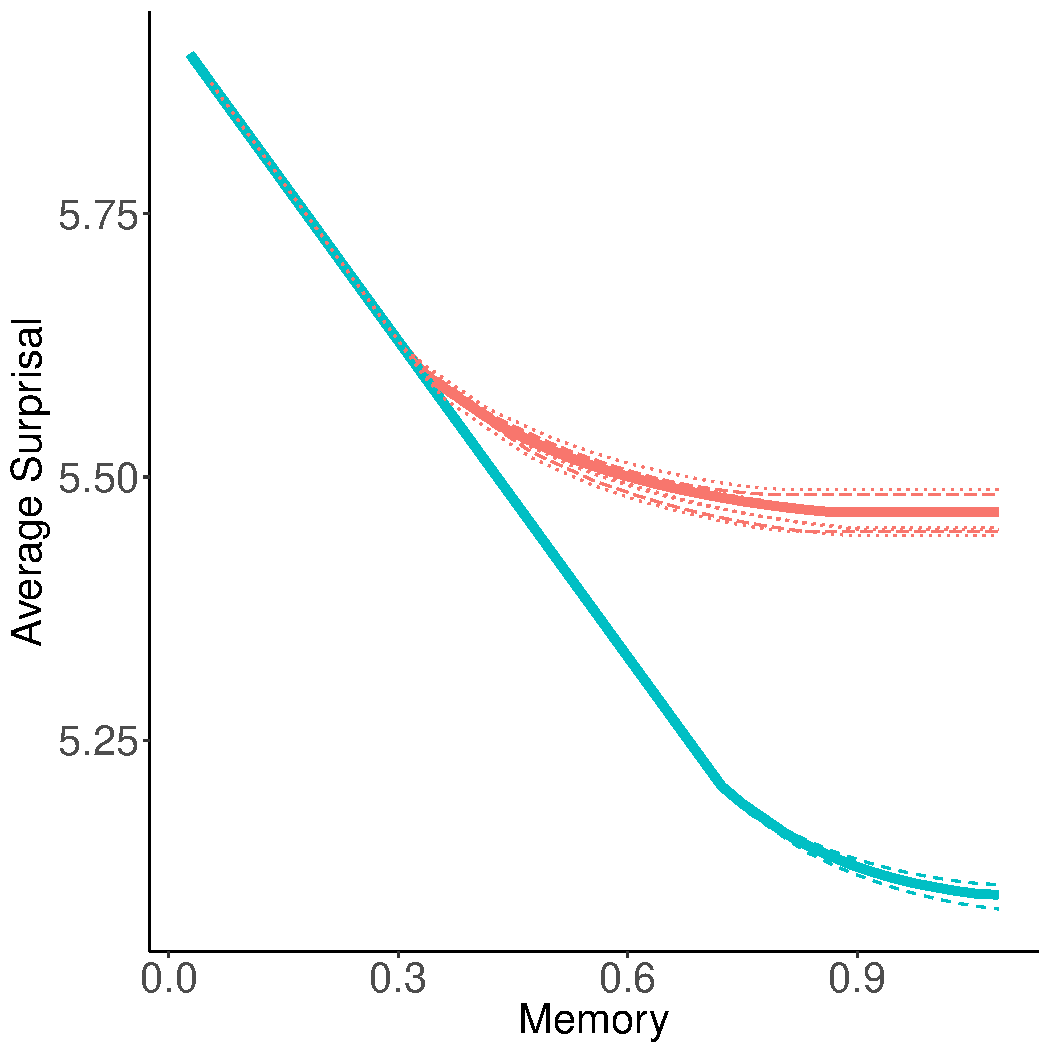
\includegraphics[width=0.25\textwidth]{neural/figures/Korean-listener-surprisal-memory-MEDIANS_QUANTILES_onlyWordForms_boundedVocab_REAL.pdf}
 \\ 

%\end{longtable}
%	\captionof{figure}{Medians (cont.)}
%\end{center}
%
%\begin{center}
%\begin{longtable}{ccccccccccccccclll}
%Kurmanji & Latvian & Maltese & Naija
 \\ 
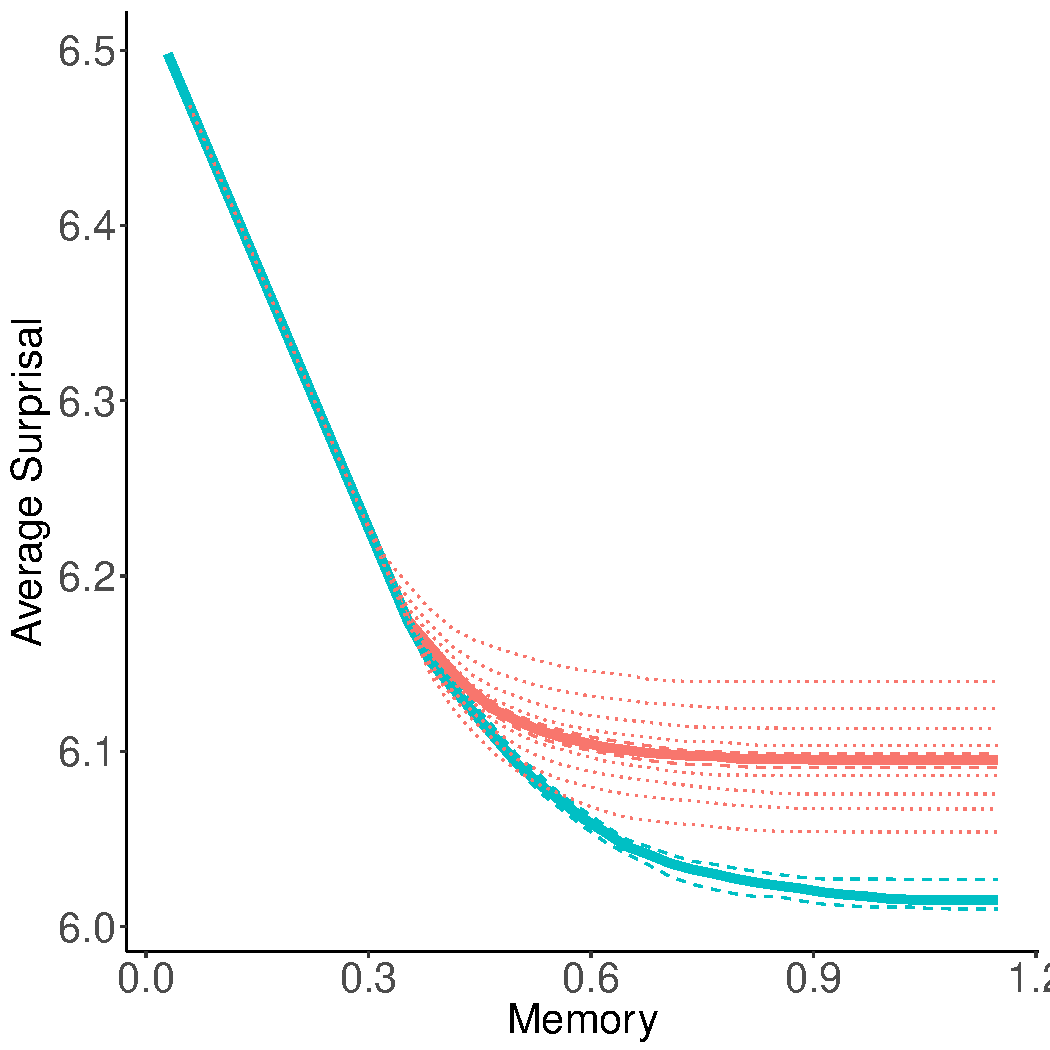
\includegraphics[width=0.25\textwidth]{neural/figures/Kurmanji-Adap-listener-surprisal-memory-MEDIANS_QUANTILES_onlyWordForms_boundedVocab_REAL.pdf} & 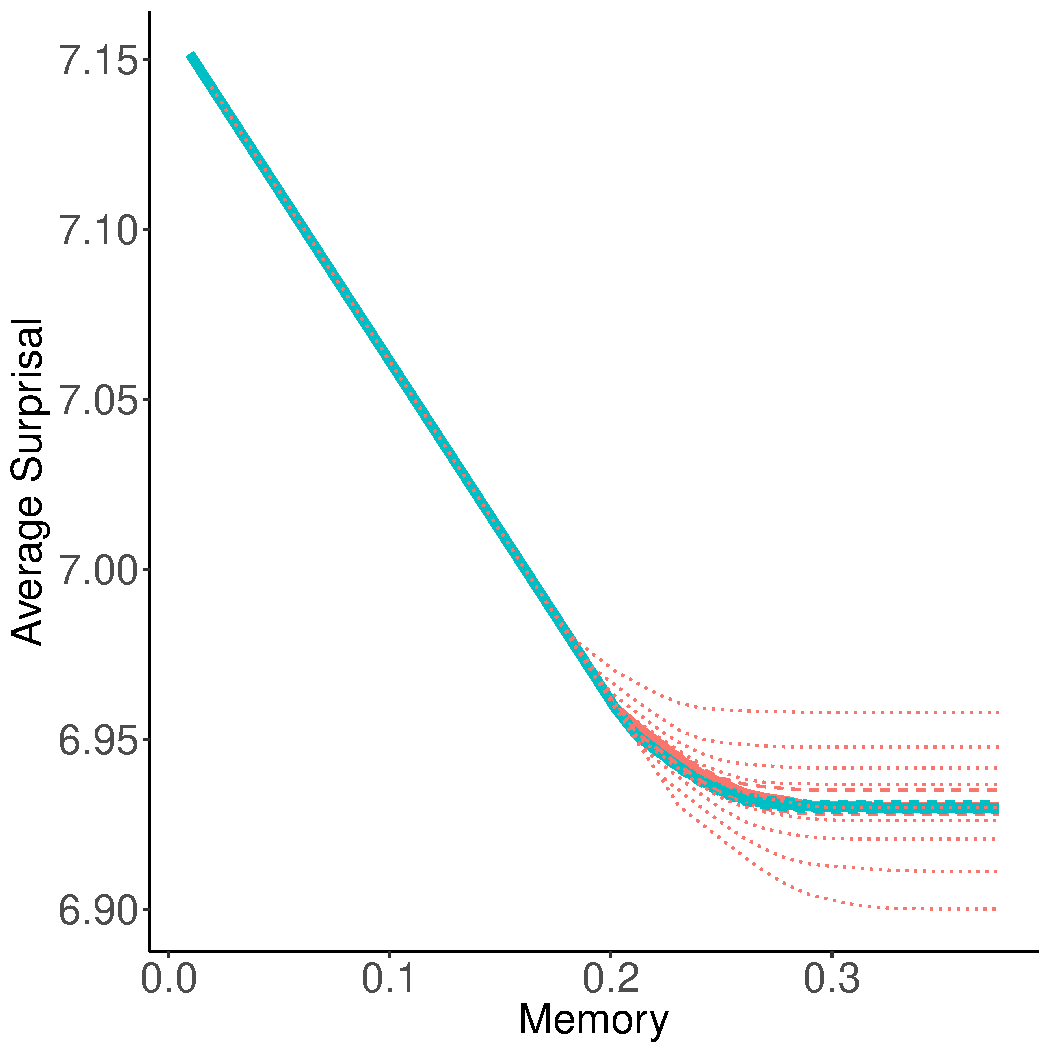
\includegraphics[width=0.25\textwidth]{neural/figures/Latvian-listener-surprisal-memory-MEDIANS_QUANTILES_onlyWordForms_boundedVocab_REAL.pdf} & 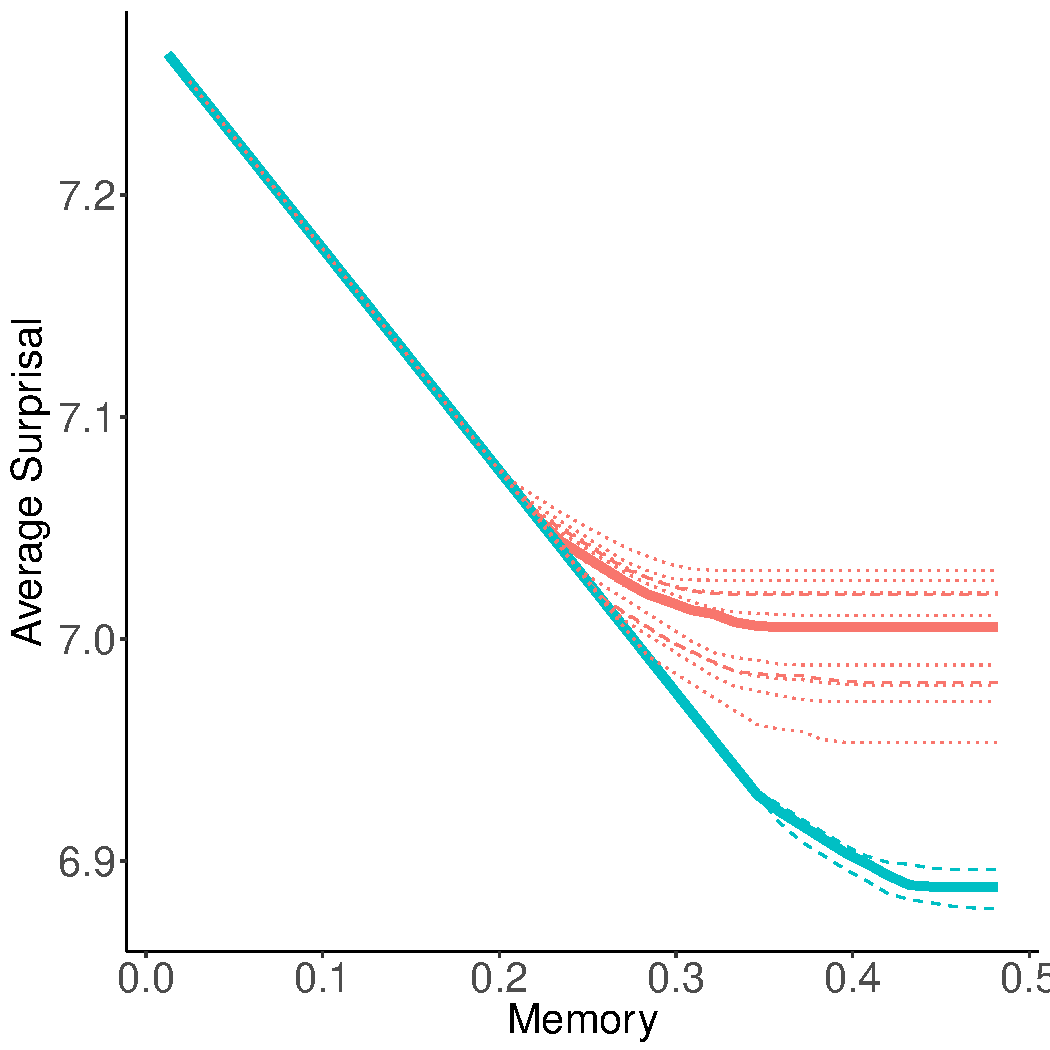
\includegraphics[width=0.25\textwidth]{neural/figures/Maltese-listener-surprisal-memory-MEDIANS_QUANTILES_onlyWordForms_boundedVocab_REAL.pdf} & 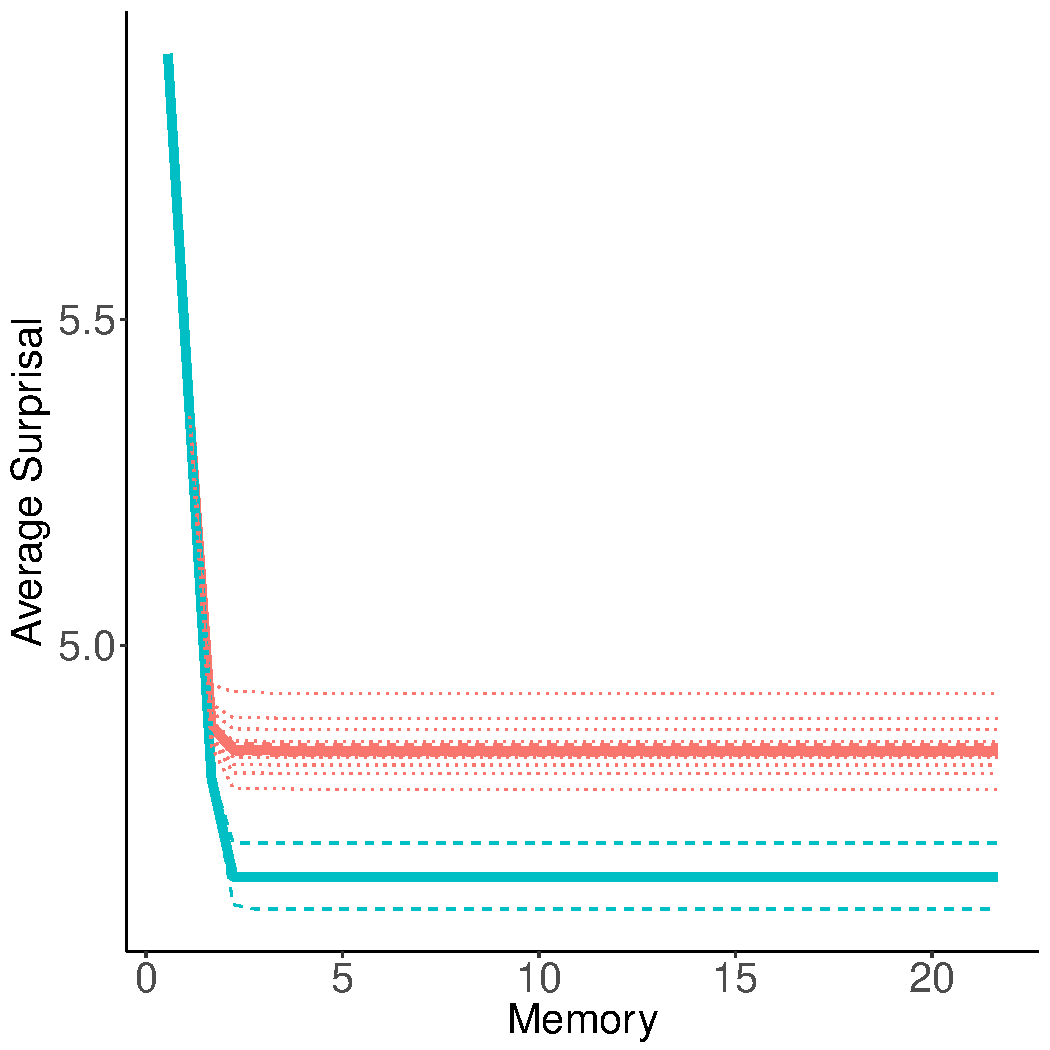
\includegraphics[width=0.25\textwidth]{neural/figures/Naija-Adap-listener-surprisal-memory-MEDIANS_QUANTILES_onlyWordForms_boundedVocab_REAL.pdf}
 \\ 
North Sami & Norwegian & Persian & Polish
 \\ 
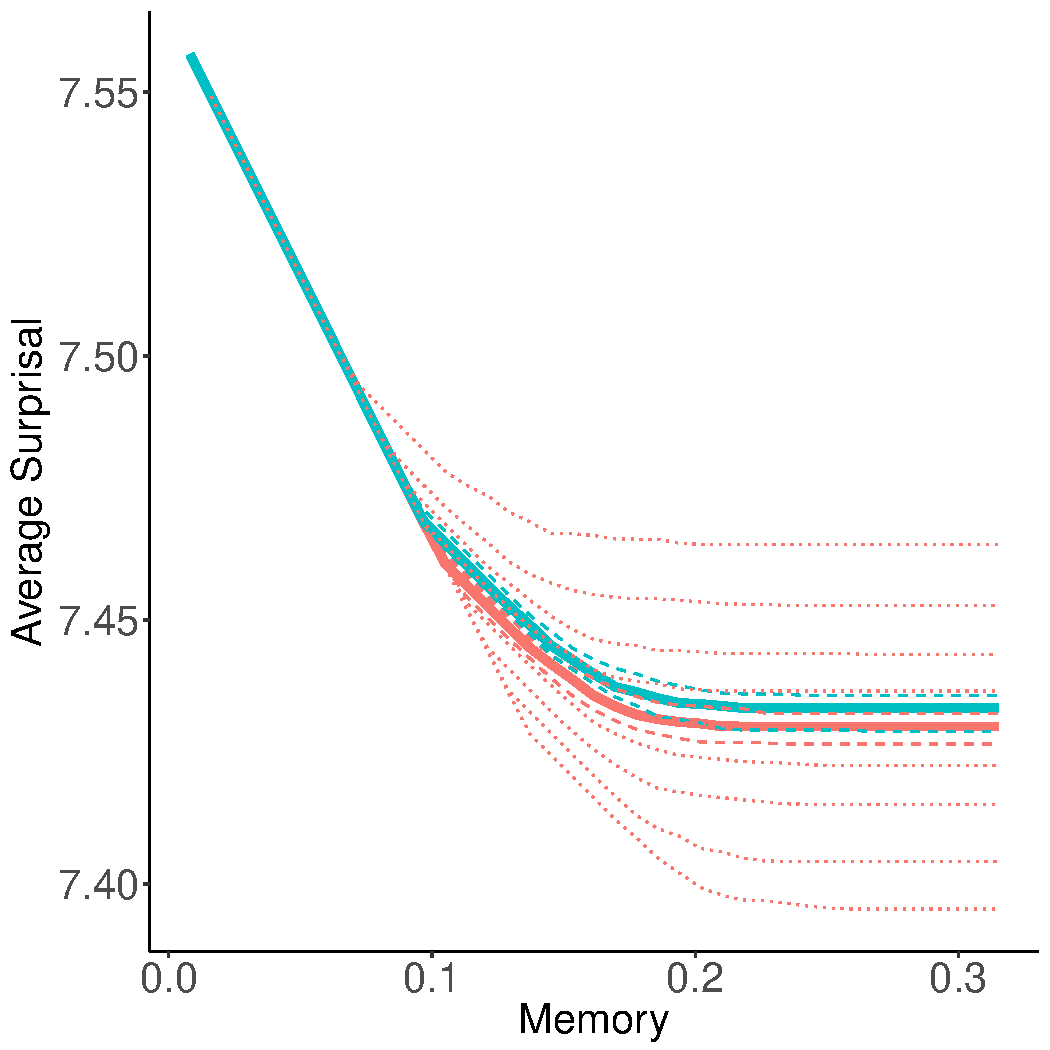
\includegraphics[width=0.25\textwidth]{neural/figures/North_Sami-listener-surprisal-memory-MEDIANS_QUANTILES_onlyWordForms_boundedVocab_REAL.pdf} & 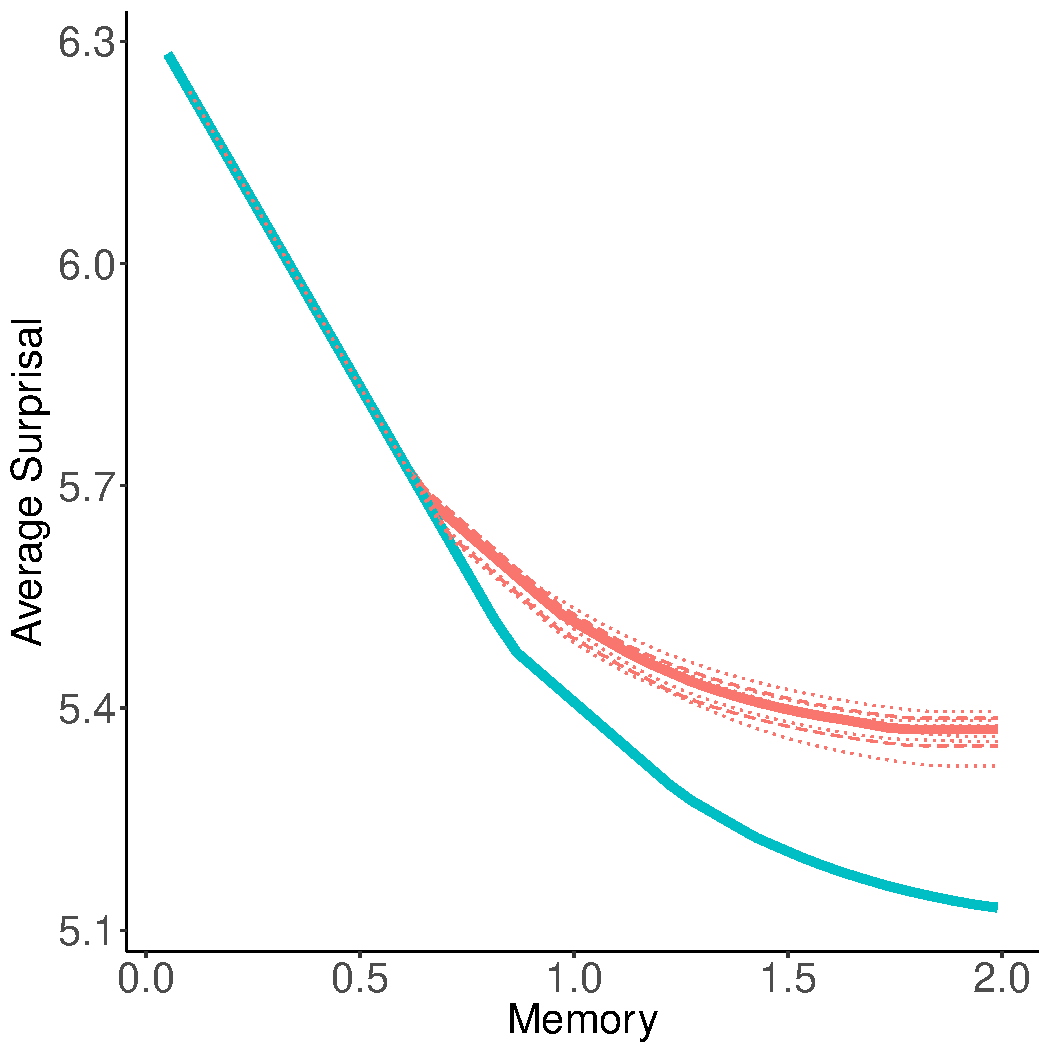
\includegraphics[width=0.25\textwidth]{neural/figures/Norwegian-listener-surprisal-memory-MEDIANS_QUANTILES_onlyWordForms_boundedVocab_REAL.pdf} & 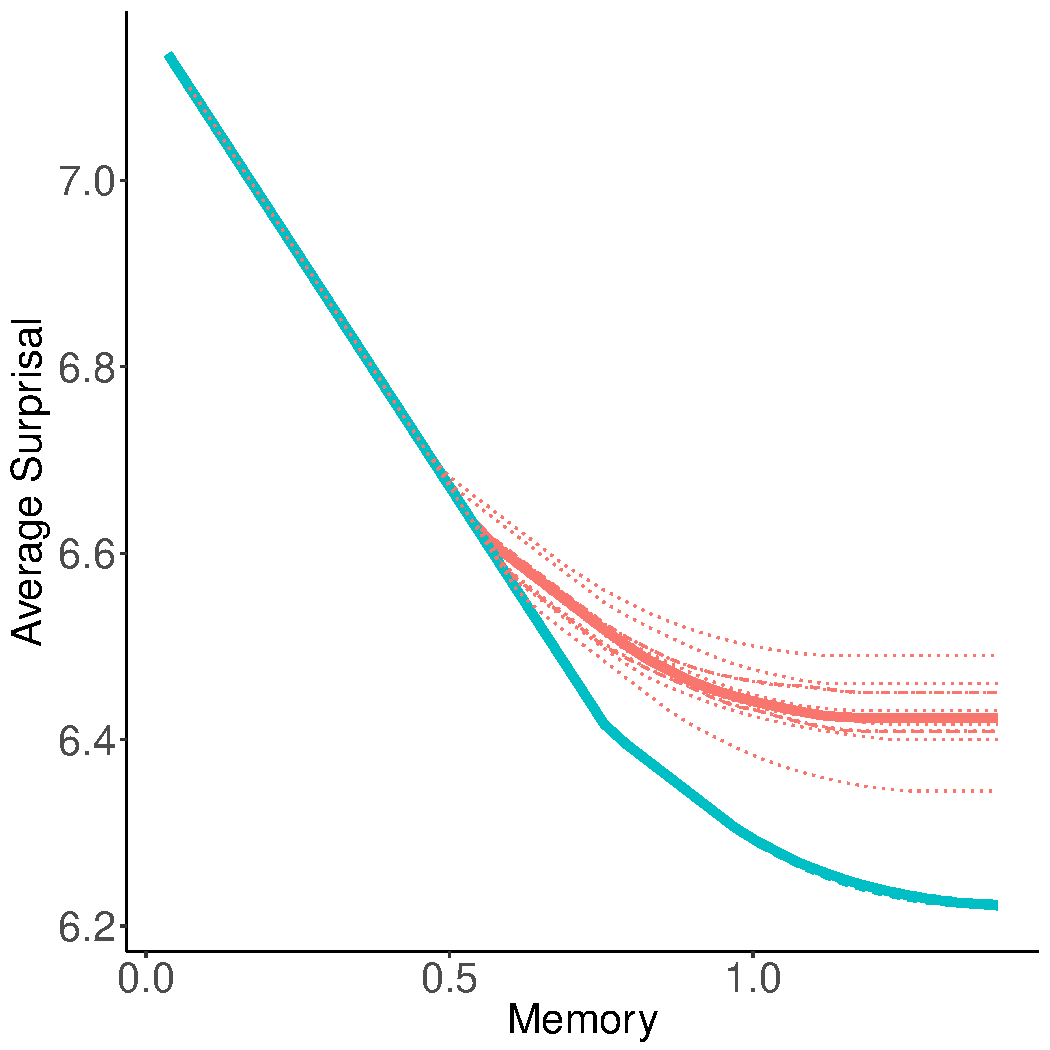
\includegraphics[width=0.25\textwidth]{neural/figures/Persian-listener-surprisal-memory-MEDIANS_QUANTILES_onlyWordForms_boundedVocab_REAL.pdf} & 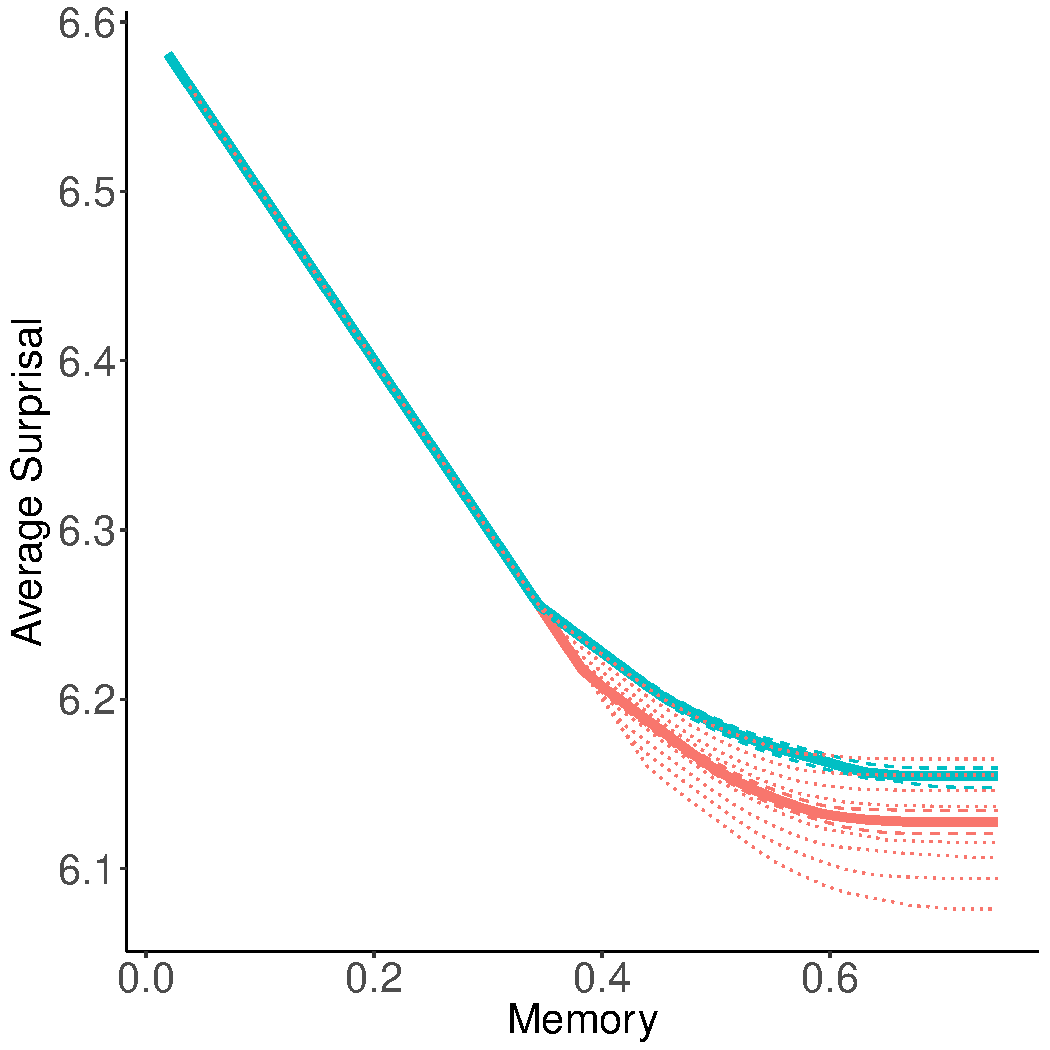
\includegraphics[width=0.25\textwidth]{neural/figures/Polish-listener-surprisal-memory-MEDIANS_QUANTILES_onlyWordForms_boundedVocab_REAL.pdf}
 \\ 
Portuguese & Romanian & Russian & Serbian
 \\ 
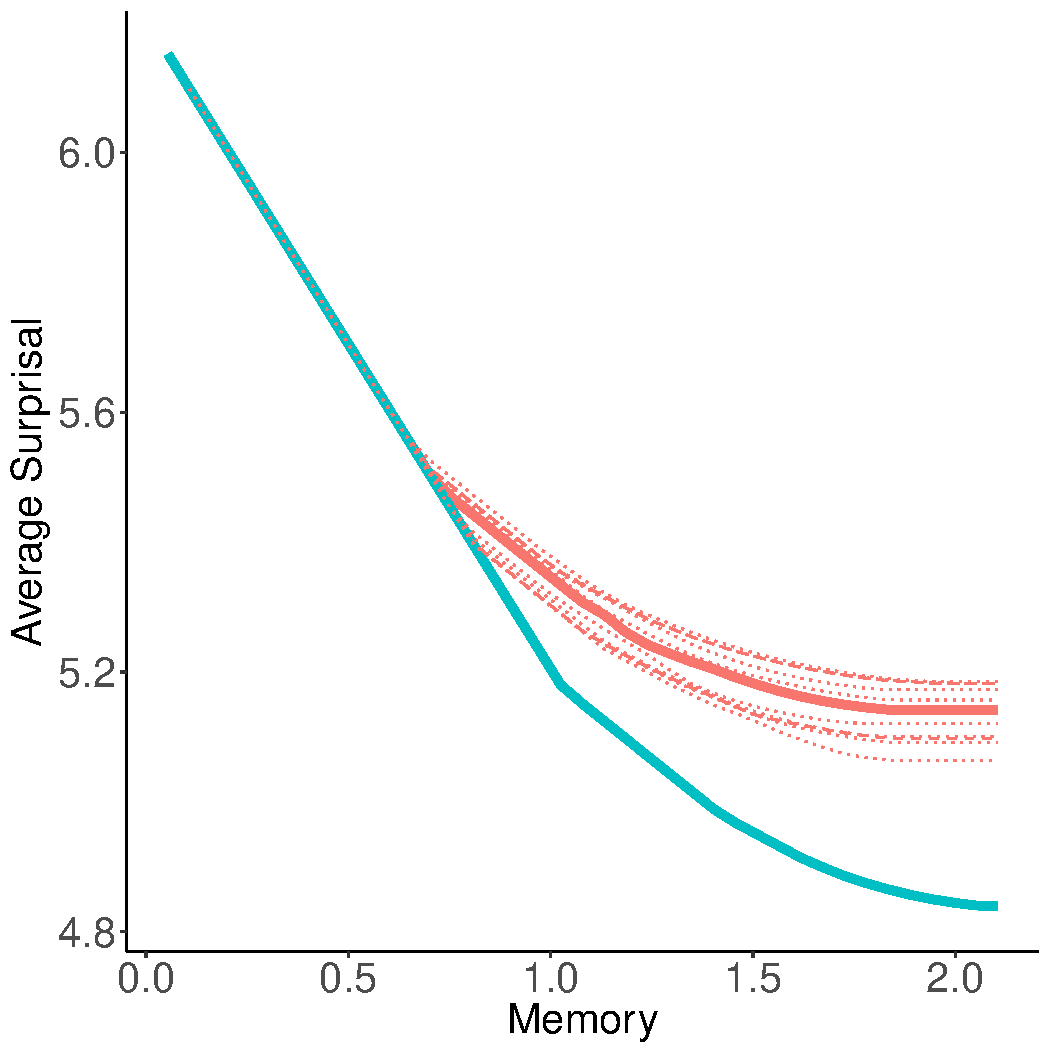
\includegraphics[width=0.25\textwidth]{neural/figures/Portuguese-listener-surprisal-memory-MEDIANS_QUANTILES_onlyWordForms_boundedVocab_REAL.pdf} & 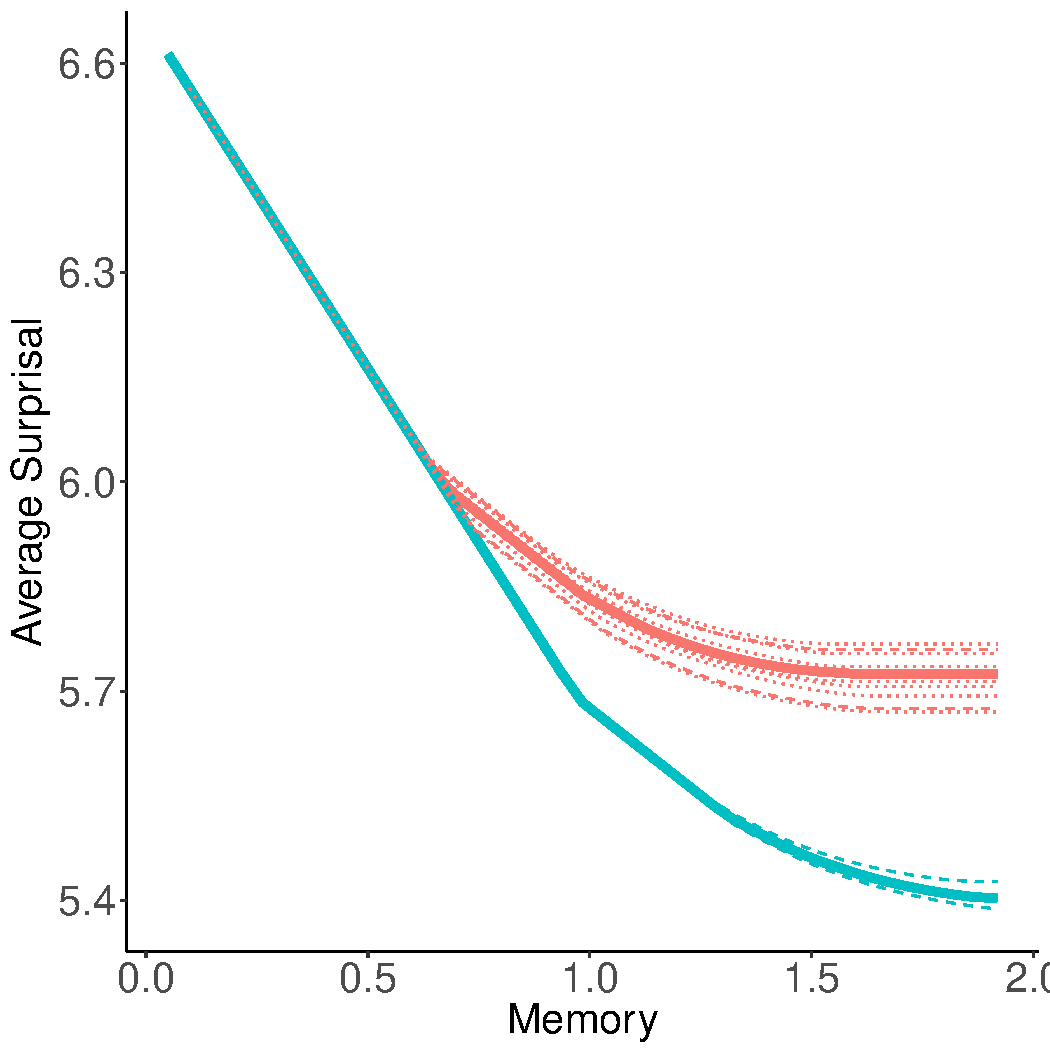
\includegraphics[width=0.25\textwidth]{neural/figures/Romanian-listener-surprisal-memory-MEDIANS_QUANTILES_onlyWordForms_boundedVocab_REAL.pdf} & 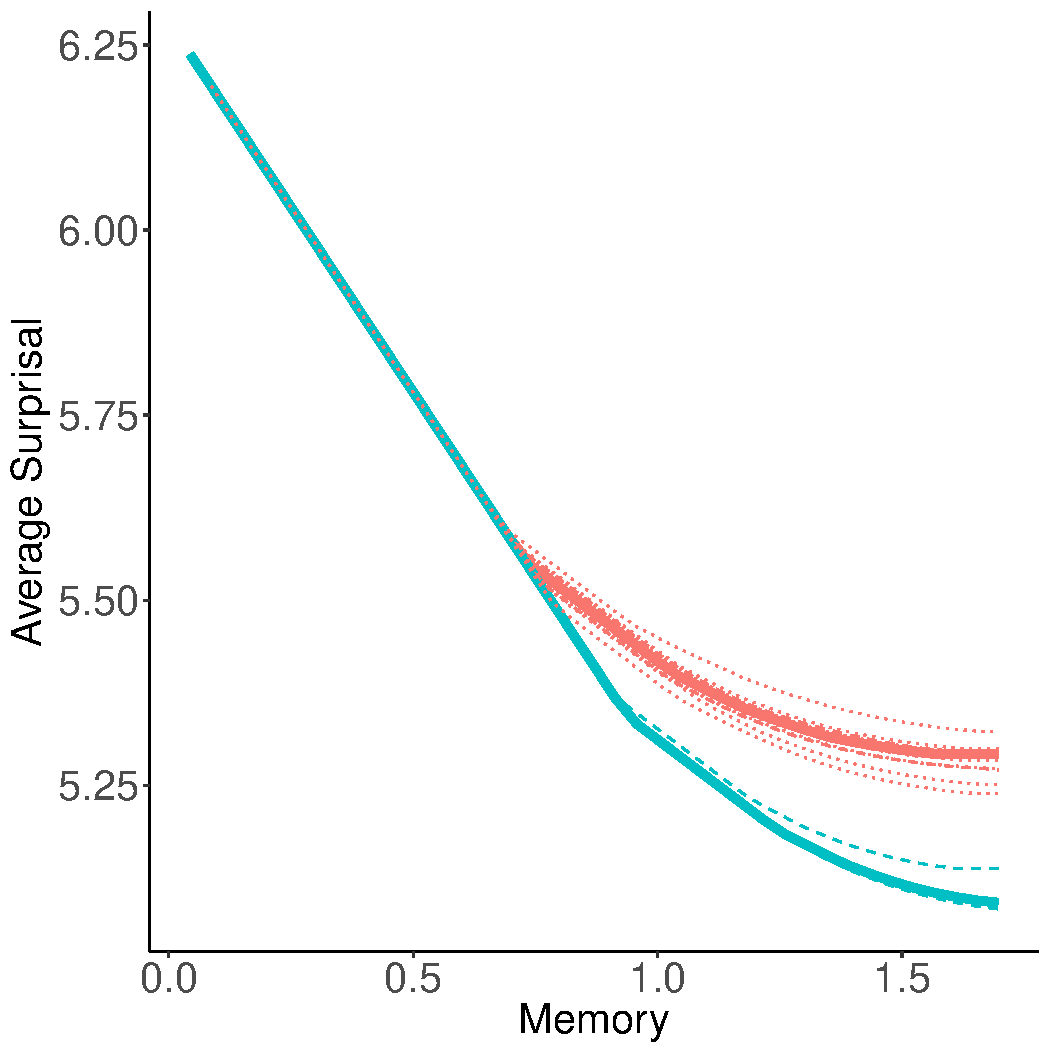
\includegraphics[width=0.25\textwidth]{neural/figures/Russian-listener-surprisal-memory-MEDIANS_QUANTILES_onlyWordForms_boundedVocab_REAL.pdf} & 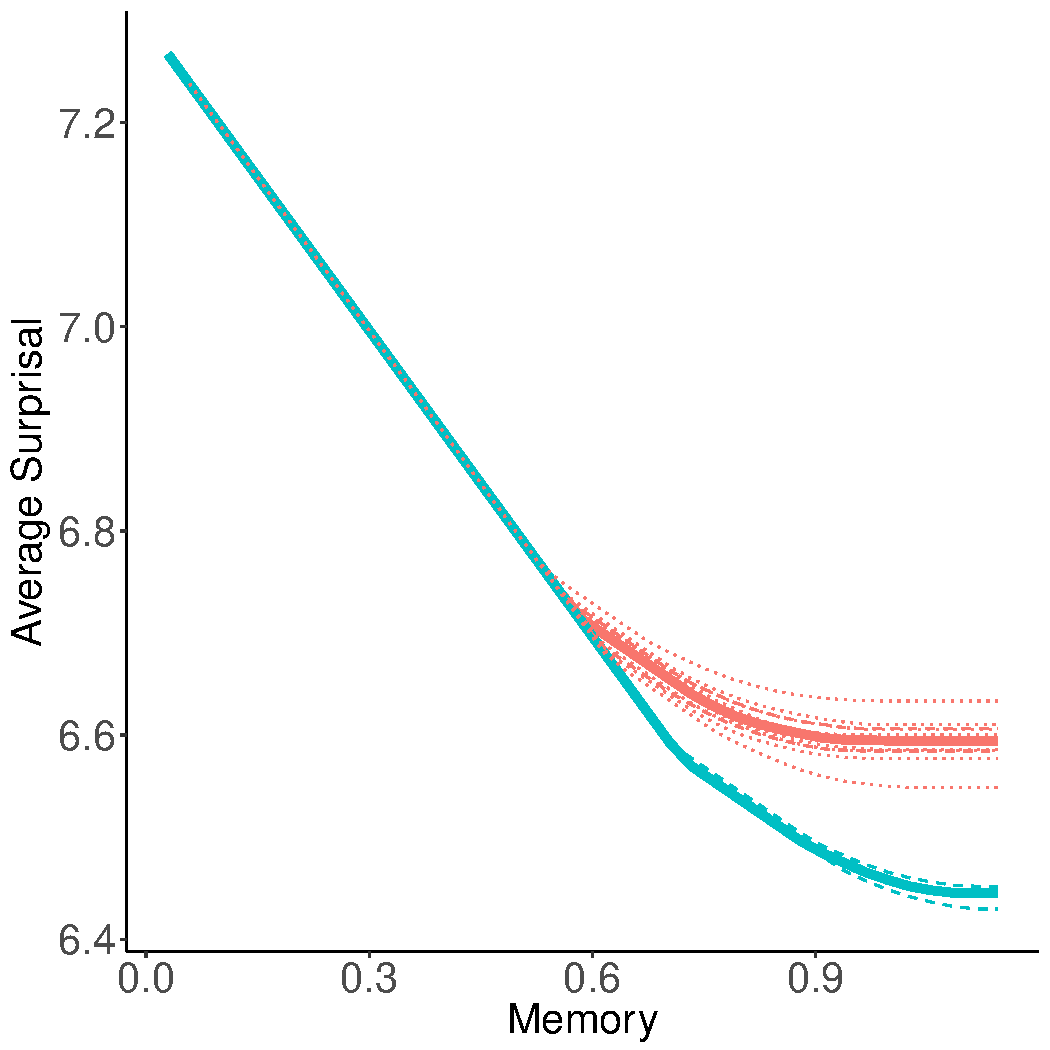
\includegraphics[width=0.25\textwidth]{neural/figures/Serbian-listener-surprisal-memory-MEDIANS_QUANTILES_onlyWordForms_boundedVocab_REAL.pdf}
 \\ 
Slovak & Slovenian & Spanish & Swedish
 \\ 
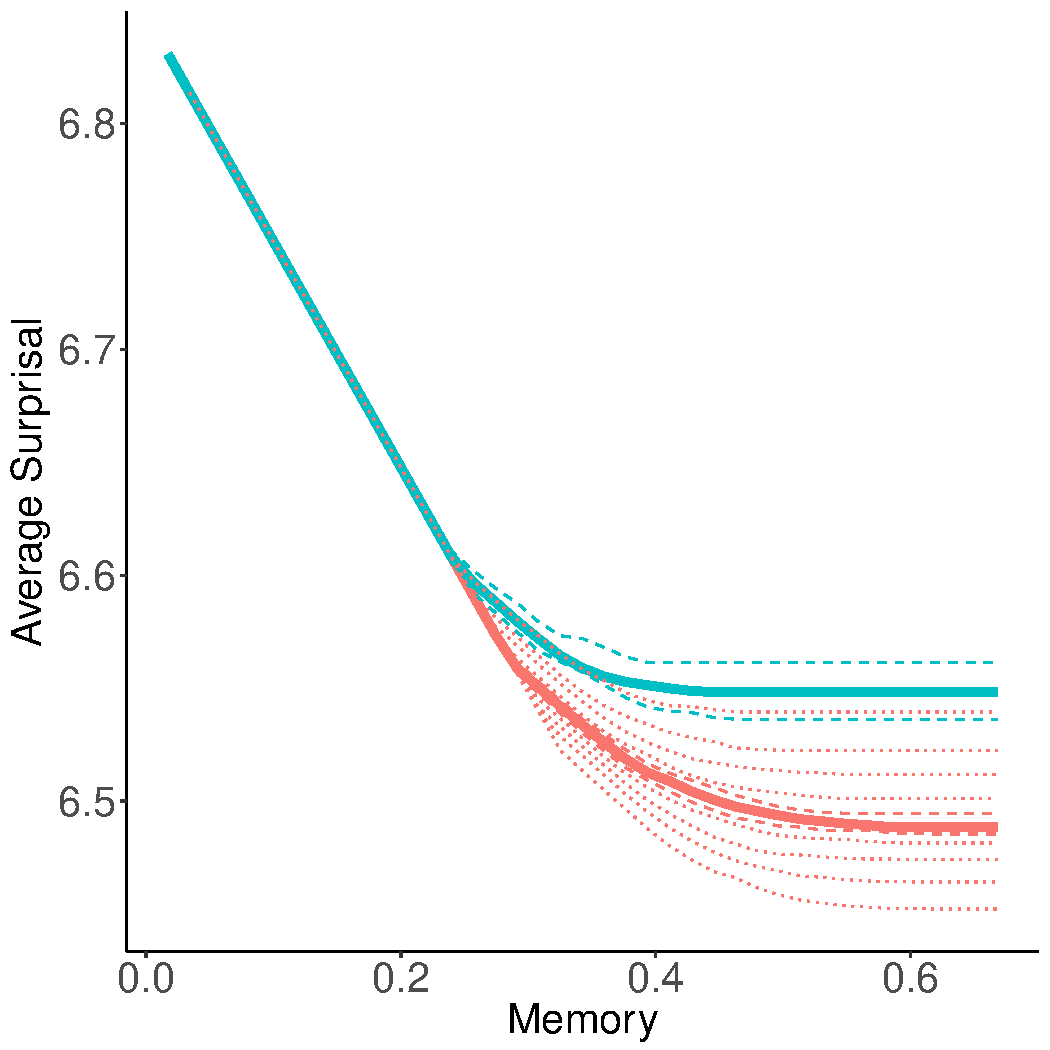
\includegraphics[width=0.25\textwidth]{neural/figures/Slovak-listener-surprisal-memory-MEDIANS_QUANTILES_onlyWordForms_boundedVocab_REAL.pdf} & 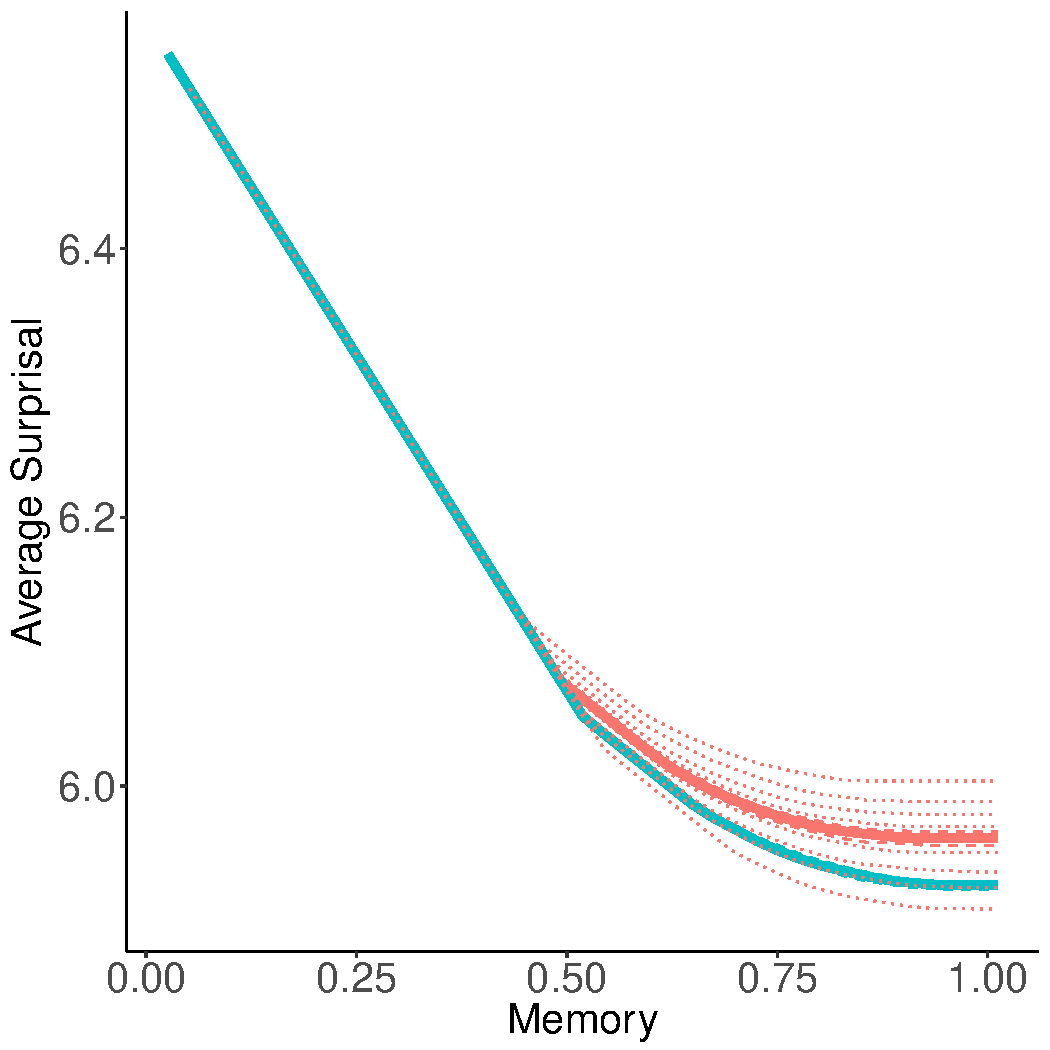
\includegraphics[width=0.25\textwidth]{neural/figures/Slovenian-listener-surprisal-memory-MEDIANS_QUANTILES_onlyWordForms_boundedVocab_REAL.pdf} & 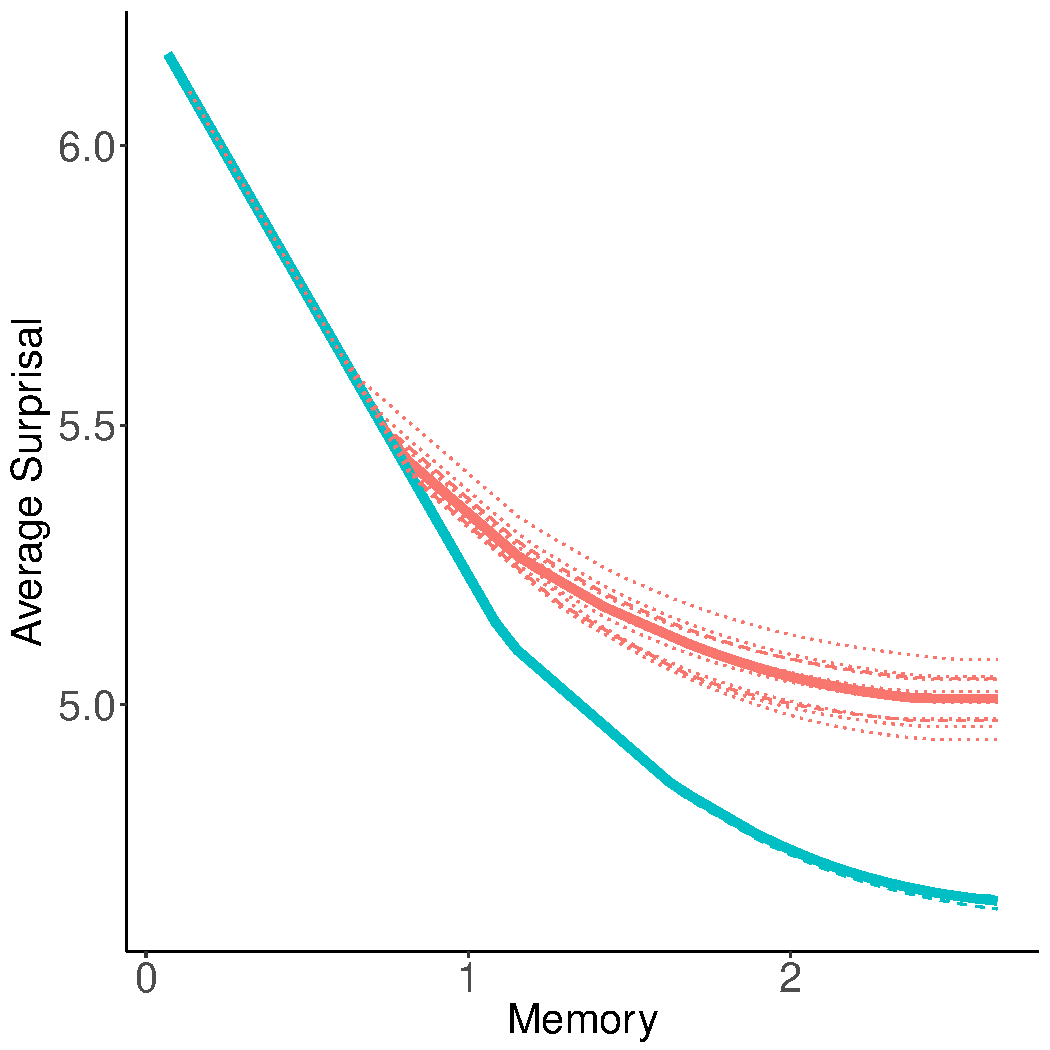
\includegraphics[width=0.25\textwidth]{neural/figures/Spanish-listener-surprisal-memory-MEDIANS_QUANTILES_onlyWordForms_boundedVocab_REAL.pdf} & 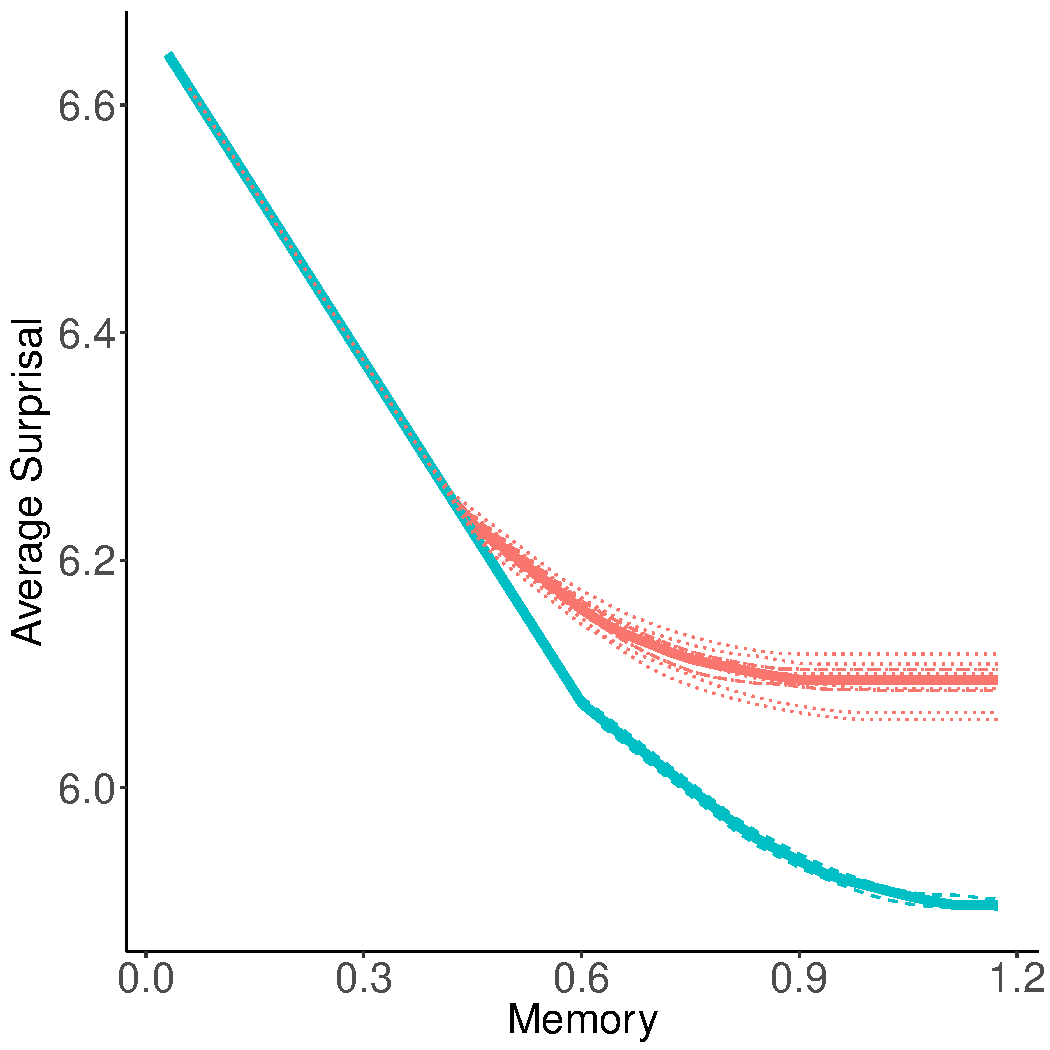
\includegraphics[width=0.25\textwidth]{neural/figures/Swedish-listener-surprisal-memory-MEDIANS_QUANTILES_onlyWordForms_boundedVocab_REAL.pdf}
 \\ 

%\end{longtable}
%	\captionof{figure}{Medians (cont.)}
%\end{center}
%
%\begin{center}
%\begin{longtable}{ccccccccccccccclll}
%Thai & Turkish & Ukrainian & Urdu
 \\ 
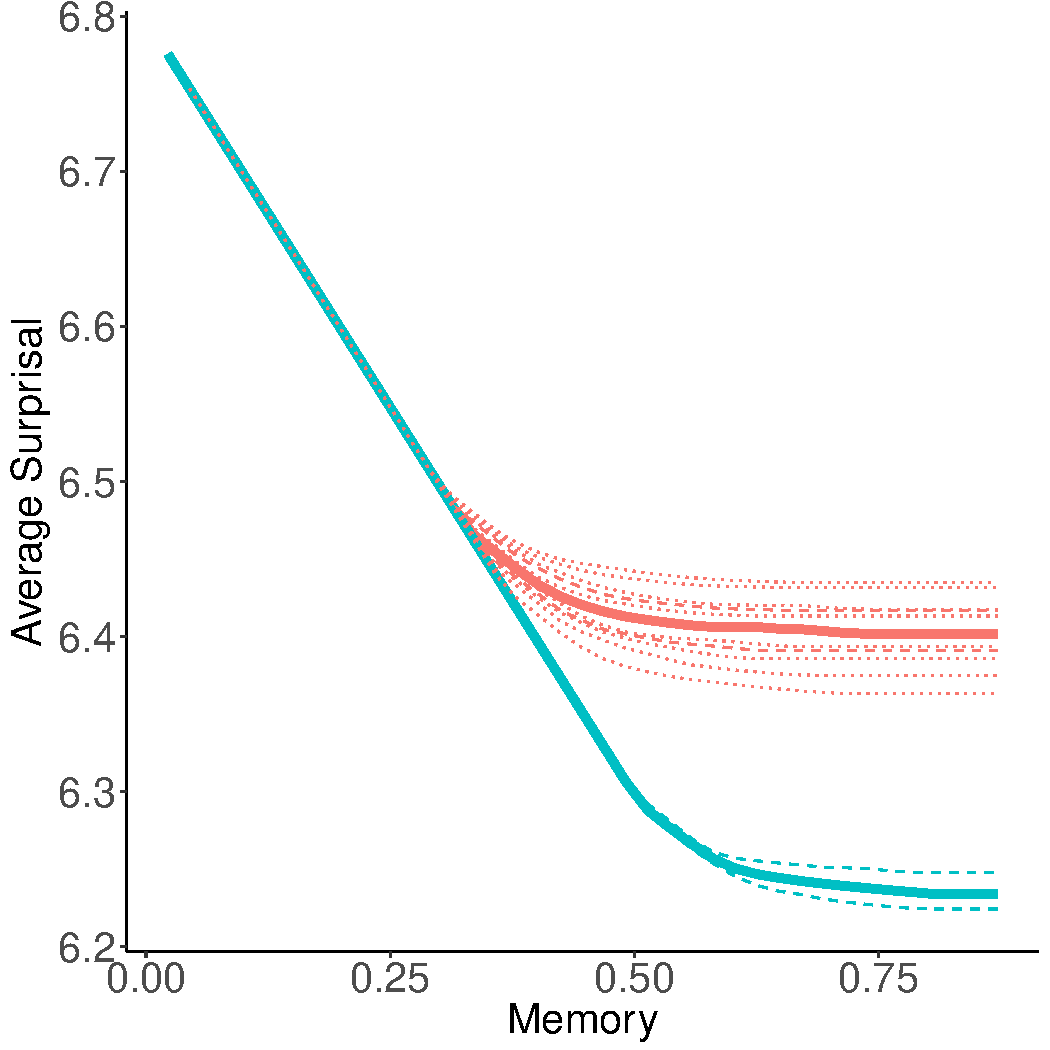
\includegraphics[width=0.25\textwidth]{neural/figures/Thai-Adap-listener-surprisal-memory-MEDIANS_QUANTILES_onlyWordForms_boundedVocab_REAL.pdf} & \includegraphics[width=0.25\textwidth]{neural/figures/Turkish-listener-surprisal-memory-MEDIANS_QUANTILES_onlyWordForms_boundedVocab_REAL.pdf} & \includegraphics[width=0.25\textwidth]{neural/figures/Ukrainian-listener-surprisal-memory-MEDIANS_QUANTILES_onlyWordForms_boundedVocab_REAL.pdf} & \includegraphics[width=0.25\textwidth]{neural/figures/Urdu-listener-surprisal-memory-MEDIANS_QUANTILES_onlyWordForms_boundedVocab_REAL.pdf}
 \\ 
Uyghur & Vietnamese &  & 
 \\ 
\includegraphics[width=0.25\textwidth]{neural/figures/Uyghur-Adap-listener-surprisal-memory-MEDIANS_QUANTILES_onlyWordForms_boundedVocab_REAL.pdf} & \includegraphics[width=0.25\textwidth]{neural/figures/Vietnamese-listener-surprisal-memory-MEDIANS_QUANTILES_onlyWordForms_boundedVocab_REAL.pdf} &  & 
 \\ 

%\end{longtable}
%	\captionof{figure}{Medians (cont.)}
%\end{center}
%


%
%\subsection{Surprisal at Maximum Memory}
%
%
%\begin{center}
%\begin{longtable}{ccccccccccccccclll}
%Afrikaans & Amharic & Arabic & Armenian
 \\ 
\includegraphics[width=0.25\textwidth]{neural/figures/Afrikaans-listener-surprisal-memory-HIST_byMem_onlyWordForms_boundedVocab_REAL.pdf} & \includegraphics[width=0.25\textwidth]{neural/figures/Amharic-Adap-listener-surprisal-memory-HIST_byMem_onlyWordForms_boundedVocab_REAL.pdf} & \includegraphics[width=0.25\textwidth]{neural/figures/Arabic-listener-surprisal-memory-HIST_byMem_onlyWordForms_boundedVocab_REAL.pdf} & \includegraphics[width=0.25\textwidth]{neural/figures/Armenian-Adap-listener-surprisal-memory-HIST_byMem_onlyWordForms_boundedVocab_REAL.pdf}
 \\ 
Bambara & Basque & Breton & Bulgarian
 \\ 
\includegraphics[width=0.25\textwidth]{neural/figures/Bambara-Adap-listener-surprisal-memory-HIST_byMem_onlyWordForms_boundedVocab_REAL.pdf} & \includegraphics[width=0.25\textwidth]{neural/figures/Basque-listener-surprisal-memory-HIST_byMem_onlyWordForms_boundedVocab_REAL.pdf} & \includegraphics[width=0.25\textwidth]{neural/figures/Breton-Adap-listener-surprisal-memory-HIST_byMem_onlyWordForms_boundedVocab_REAL.pdf} & \includegraphics[width=0.25\textwidth]{neural/figures/Bulgarian-listener-surprisal-memory-HIST_byMem_onlyWordForms_boundedVocab_REAL.pdf}
 \\ 
Buryat & Cantonese & Catalan & Chinese
 \\ 
\includegraphics[width=0.25\textwidth]{neural/figures/Buryat-Adap-listener-surprisal-memory-HIST_byMem_onlyWordForms_boundedVocab_REAL.pdf} & \includegraphics[width=0.25\textwidth]{neural/figures/Cantonese-Adap-listener-surprisal-memory-HIST_byMem_onlyWordForms_boundedVocab_REAL.pdf} & \includegraphics[width=0.25\textwidth]{neural/figures/Catalan-listener-surprisal-memory-HIST_byMem_onlyWordForms_boundedVocab_REAL.pdf} & \includegraphics[width=0.25\textwidth]{neural/figures/Chinese-listener-surprisal-memory-HIST_byMem_onlyWordForms_boundedVocab_REAL.pdf}
 \\ 
Croatian & Czech & Danish & Dutch
 \\ 
\includegraphics[width=0.25\textwidth]{neural/figures/Croatian-listener-surprisal-memory-HIST_byMem_onlyWordForms_boundedVocab_REAL.pdf} & \includegraphics[width=0.25\textwidth]{neural/figures/Czech-listener-surprisal-memory-HIST_byMem_onlyWordForms_boundedVocab_REAL.pdf} & \includegraphics[width=0.25\textwidth]{neural/figures/Danish-listener-surprisal-memory-HIST_byMem_onlyWordForms_boundedVocab_REAL.pdf} & \includegraphics[width=0.25\textwidth]{neural/figures/Dutch-listener-surprisal-memory-HIST_byMem_onlyWordForms_boundedVocab_REAL.pdf}
 \\ 

%English & Erzya & Estonian & Faroese
 \\ 
\includegraphics[width=0.25\textwidth]{neural/figures/English-listener-surprisal-memory-HIST_byMem_onlyWordForms_boundedVocab_REAL.pdf} & \includegraphics[width=0.25\textwidth]{neural/figures/Erzya-Adap-listener-surprisal-memory-HIST_byMem_onlyWordForms_boundedVocab_REAL.pdf} & \includegraphics[width=0.25\textwidth]{neural/figures/Estonian-listener-surprisal-memory-HIST_byMem_onlyWordForms_boundedVocab_REAL.pdf} & \includegraphics[width=0.25\textwidth]{neural/figures/Faroese-Adap-listener-surprisal-memory-HIST_byMem_onlyWordForms_boundedVocab_REAL.pdf}
 \\ 
Finnish & French & German & Greek
 \\ 
\includegraphics[width=0.25\textwidth]{neural/figures/Finnish-listener-surprisal-memory-HIST_byMem_onlyWordForms_boundedVocab_REAL.pdf} & \includegraphics[width=0.25\textwidth]{neural/figures/French-listener-surprisal-memory-HIST_byMem_onlyWordForms_boundedVocab_REAL.pdf} & \includegraphics[width=0.25\textwidth]{neural/figures/German-listener-surprisal-memory-HIST_byMem_onlyWordForms_boundedVocab_REAL.pdf} & \includegraphics[width=0.25\textwidth]{neural/figures/Greek-listener-surprisal-memory-HIST_byMem_onlyWordForms_boundedVocab_REAL.pdf}
 \\ 
Hebrew & Hindi & Hungarian & Indonesian
 \\ 
\includegraphics[width=0.25\textwidth]{neural/figures/Hebrew-listener-surprisal-memory-HIST_byMem_onlyWordForms_boundedVocab_REAL.pdf} & \includegraphics[width=0.25\textwidth]{neural/figures/Hindi-listener-surprisal-memory-HIST_byMem_onlyWordForms_boundedVocab_REAL.pdf} & \includegraphics[width=0.25\textwidth]{neural/figures/Hungarian-listener-surprisal-memory-HIST_byMem_onlyWordForms_boundedVocab_REAL.pdf} & \includegraphics[width=0.25\textwidth]{neural/figures/Indonesian-listener-surprisal-memory-HIST_byMem_onlyWordForms_boundedVocab_REAL.pdf}
 \\ 
Italian & Japanese & Kazakh & Korean
 \\ 
\includegraphics[width=0.25\textwidth]{neural/figures/Italian-listener-surprisal-memory-HIST_byMem_onlyWordForms_boundedVocab_REAL.pdf} & \includegraphics[width=0.25\textwidth]{neural/figures/Japanese-listener-surprisal-memory-HIST_byMem_onlyWordForms_boundedVocab_REAL.pdf} & \includegraphics[width=0.25\textwidth]{neural/figures/Kazakh-Adap-listener-surprisal-memory-HIST_byMem_onlyWordForms_boundedVocab_REAL.pdf} & \includegraphics[width=0.25\textwidth]{neural/figures/Korean-listener-surprisal-memory-HIST_byMem_onlyWordForms_boundedVocab_REAL.pdf}
 \\ 

%Kurmanji & Latvian & Maltese & Naija
 \\ 
\includegraphics[width=0.25\textwidth]{neural/figures/Kurmanji-Adap-listener-surprisal-memory-HIST_byMem_onlyWordForms_boundedVocab_REAL.pdf} & \includegraphics[width=0.25\textwidth]{neural/figures/Latvian-listener-surprisal-memory-HIST_byMem_onlyWordForms_boundedVocab_REAL.pdf} & \includegraphics[width=0.25\textwidth]{neural/figures/Maltese-listener-surprisal-memory-HIST_byMem_onlyWordForms_boundedVocab_REAL.pdf} & \includegraphics[width=0.25\textwidth]{neural/figures/Naija-Adap-listener-surprisal-memory-HIST_byMem_onlyWordForms_boundedVocab_REAL.pdf}
 \\ 
North Sami & Norwegian & Persian & Polish
 \\ 
\includegraphics[width=0.25\textwidth]{neural/figures/North_Sami-listener-surprisal-memory-HIST_byMem_onlyWordForms_boundedVocab_REAL.pdf} & \includegraphics[width=0.25\textwidth]{neural/figures/Norwegian-listener-surprisal-memory-HIST_byMem_onlyWordForms_boundedVocab_REAL.pdf} & \includegraphics[width=0.25\textwidth]{neural/figures/Persian-listener-surprisal-memory-HIST_byMem_onlyWordForms_boundedVocab_REAL.pdf} & \includegraphics[width=0.25\textwidth]{neural/figures/Polish-listener-surprisal-memory-HIST_byMem_onlyWordForms_boundedVocab_REAL.pdf}
 \\ 
Portuguese & Romanian & Russian & Serbian
 \\ 
\includegraphics[width=0.25\textwidth]{neural/figures/Portuguese-listener-surprisal-memory-HIST_byMem_onlyWordForms_boundedVocab_REAL.pdf} & \includegraphics[width=0.25\textwidth]{neural/figures/Romanian-listener-surprisal-memory-HIST_byMem_onlyWordForms_boundedVocab_REAL.pdf} & \includegraphics[width=0.25\textwidth]{neural/figures/Russian-listener-surprisal-memory-HIST_byMem_onlyWordForms_boundedVocab_REAL.pdf} & \includegraphics[width=0.25\textwidth]{neural/figures/Serbian-listener-surprisal-memory-HIST_byMem_onlyWordForms_boundedVocab_REAL.pdf}
 \\ 
Slovak & Slovenian & Spanish & Swedish
 \\ 
\includegraphics[width=0.25\textwidth]{neural/figures/Slovak-listener-surprisal-memory-HIST_byMem_onlyWordForms_boundedVocab_REAL.pdf} & \includegraphics[width=0.25\textwidth]{neural/figures/Slovenian-listener-surprisal-memory-HIST_byMem_onlyWordForms_boundedVocab_REAL.pdf} & \includegraphics[width=0.25\textwidth]{neural/figures/Spanish-listener-surprisal-memory-HIST_byMem_onlyWordForms_boundedVocab_REAL.pdf} & \includegraphics[width=0.25\textwidth]{neural/figures/Swedish-listener-surprisal-memory-HIST_byMem_onlyWordForms_boundedVocab_REAL.pdf}
 \\ 

%Thai & Turkish & Ukrainian & Urdu
 \\ 
\includegraphics[width=0.25\textwidth]{neural/figures/Thai-Adap-listener-surprisal-memory-HIST_byMem_onlyWordForms_boundedVocab_REAL.pdf} & \includegraphics[width=0.25\textwidth]{neural/figures/Turkish-listener-surprisal-memory-HIST_byMem_onlyWordForms_boundedVocab_REAL.pdf} & \includegraphics[width=0.25\textwidth]{neural/figures/Ukrainian-listener-surprisal-memory-HIST_byMem_onlyWordForms_boundedVocab_REAL.pdf} & \includegraphics[width=0.25\textwidth]{neural/figures/Urdu-listener-surprisal-memory-HIST_byMem_onlyWordForms_boundedVocab_REAL.pdf}
 \\ 
Uyghur & Vietnamese &  & 
 \\ 
\includegraphics[width=0.25\textwidth]{neural/figures/Uyghur-Adap-listener-surprisal-memory-HIST_byMem_onlyWordForms_boundedVocab_REAL.pdf} & \includegraphics[width=0.25\textwidth]{neural/figures/Vietnamese-listener-surprisal-memory-HIST_byMem_onlyWordForms_boundedVocab_REAL.pdf} &  & 
 \\ 

%\end{longtable}
%	\captionof{figure}{Histograms: Surprisal, at maximum memory.}\label{tab:slice-hists-real}
%\end{center}
%

%\begin{table}
%\begin{tabular}{cccccccccccccccccc}
%Afrikaans & Amharic & Arabic & Armenian
 \\ 
\includegraphics[width=0.25\textwidth]{neural/figures/Afrikaans-listener-surprisal-memory-QUANTILES_onlyWordForms_boundedVocab_REAL.pdf} & \includegraphics[width=0.25\textwidth]{neural/figures/Amharic-Adap-listener-surprisal-memory-QUANTILES_onlyWordForms_boundedVocab_REAL.pdf} & \includegraphics[width=0.25\textwidth]{neural/figures/Arabic-listener-surprisal-memory-QUANTILES_onlyWordForms_boundedVocab_REAL.pdf} & \includegraphics[width=0.25\textwidth]{neural/figures/Armenian-Adap-listener-surprisal-memory-QUANTILES_onlyWordForms_boundedVocab_REAL.pdf}
 \\ 
Bambara & Basque & Breton & Bulgarian
 \\ 
\includegraphics[width=0.25\textwidth]{neural/figures/Bambara-Adap-listener-surprisal-memory-QUANTILES_onlyWordForms_boundedVocab_REAL.pdf} & \includegraphics[width=0.25\textwidth]{neural/figures/Basque-listener-surprisal-memory-QUANTILES_onlyWordForms_boundedVocab_REAL.pdf} & \includegraphics[width=0.25\textwidth]{neural/figures/Breton-Adap-listener-surprisal-memory-QUANTILES_onlyWordForms_boundedVocab_REAL.pdf} & \includegraphics[width=0.25\textwidth]{neural/figures/Bulgarian-listener-surprisal-memory-QUANTILES_onlyWordForms_boundedVocab_REAL.pdf}
 \\ 
Buryat & Cantonese & Catalan & Chinese
 \\ 
\includegraphics[width=0.25\textwidth]{neural/figures/Buryat-Adap-listener-surprisal-memory-QUANTILES_onlyWordForms_boundedVocab_REAL.pdf} & \includegraphics[width=0.25\textwidth]{neural/figures/Cantonese-Adap-listener-surprisal-memory-QUANTILES_onlyWordForms_boundedVocab_REAL.pdf} & \includegraphics[width=0.25\textwidth]{neural/figures/Catalan-listener-surprisal-memory-QUANTILES_onlyWordForms_boundedVocab_REAL.pdf} & \includegraphics[width=0.25\textwidth]{neural/figures/Chinese-listener-surprisal-memory-QUANTILES_onlyWordForms_boundedVocab_REAL.pdf}
 \\ 
Croatian & Czech & Danish & Dutch
 \\ 
\includegraphics[width=0.25\textwidth]{neural/figures/Croatian-listener-surprisal-memory-QUANTILES_onlyWordForms_boundedVocab_REAL.pdf} & \includegraphics[width=0.25\textwidth]{neural/figures/Czech-listener-surprisal-memory-QUANTILES_onlyWordForms_boundedVocab_REAL.pdf} & \includegraphics[width=0.25\textwidth]{neural/figures/Danish-listener-surprisal-memory-QUANTILES_onlyWordForms_boundedVocab_REAL.pdf} & \includegraphics[width=0.25\textwidth]{neural/figures/Dutch-listener-surprisal-memory-QUANTILES_onlyWordForms_boundedVocab_REAL.pdf}
 \\ 
English & Erzya & Estonian & Faroese
 \\ 
\includegraphics[width=0.25\textwidth]{neural/figures/English-listener-surprisal-memory-QUANTILES_onlyWordForms_boundedVocab_REAL.pdf} & \includegraphics[width=0.25\textwidth]{neural/figures/Erzya-Adap-listener-surprisal-memory-QUANTILES_onlyWordForms_boundedVocab_REAL.pdf} & \includegraphics[width=0.25\textwidth]{neural/figures/Estonian-listener-surprisal-memory-QUANTILES_onlyWordForms_boundedVocab_REAL.pdf} & \includegraphics[width=0.25\textwidth]{neural/figures/Faroese-Adap-listener-surprisal-memory-QUANTILES_onlyWordForms_boundedVocab_REAL.pdf}
 \\ 

%\end{tabular}
%	\captionof{figure}{Quantiles: At a given memory budget, what percentage of the baselines results in higher listener surprisal than the real language? Solid curves represent sample means, dashed lines represent 95 \% confidence bounds; dotted lines represent 99.9 \% confidence bounds. At five evenly spaced memory levels, we provide a p-value for the null hypothesis that the actual population mean is $0.5$ or less. Confidence bounds and p-values are obtained using an exact nonparametric method (see text).}\label{tab:quantiles}
%\end{center}
%
%\begin{table}
%\begin{tabular}{cccccccccccccccccc}
%Finnish & French & German & Greek
 \\ 
\includegraphics[width=0.25\textwidth]{neural/figures/Finnish-listener-surprisal-memory-QUANTILES_onlyWordForms_boundedVocab_REAL.pdf} & \includegraphics[width=0.25\textwidth]{neural/figures/French-listener-surprisal-memory-QUANTILES_onlyWordForms_boundedVocab_REAL.pdf} & \includegraphics[width=0.25\textwidth]{neural/figures/German-listener-surprisal-memory-QUANTILES_onlyWordForms_boundedVocab_REAL.pdf} & \includegraphics[width=0.25\textwidth]{neural/figures/Greek-listener-surprisal-memory-QUANTILES_onlyWordForms_boundedVocab_REAL.pdf}
 \\ 
Hebrew & Hindi & Hungarian & Indonesian
 \\ 
\includegraphics[width=0.25\textwidth]{neural/figures/Hebrew-listener-surprisal-memory-QUANTILES_onlyWordForms_boundedVocab_REAL.pdf} & \includegraphics[width=0.25\textwidth]{neural/figures/Hindi-listener-surprisal-memory-QUANTILES_onlyWordForms_boundedVocab_REAL.pdf} & \includegraphics[width=0.25\textwidth]{neural/figures/Hungarian-listener-surprisal-memory-QUANTILES_onlyWordForms_boundedVocab_REAL.pdf} & \includegraphics[width=0.25\textwidth]{neural/figures/Indonesian-listener-surprisal-memory-QUANTILES_onlyWordForms_boundedVocab_REAL.pdf}
 \\ 
Italian & Japanese & Kazakh & Korean
 \\ 
\includegraphics[width=0.25\textwidth]{neural/figures/Italian-listener-surprisal-memory-QUANTILES_onlyWordForms_boundedVocab_REAL.pdf} & \includegraphics[width=0.25\textwidth]{neural/figures/Japanese-listener-surprisal-memory-QUANTILES_onlyWordForms_boundedVocab_REAL.pdf} & \includegraphics[width=0.25\textwidth]{neural/figures/Kazakh-Adap-listener-surprisal-memory-QUANTILES_onlyWordForms_boundedVocab_REAL.pdf} & \includegraphics[width=0.25\textwidth]{neural/figures/Korean-listener-surprisal-memory-QUANTILES_onlyWordForms_boundedVocab_REAL.pdf}
 \\ 
Kurmanji & Latvian & Maltese & Naija
 \\ 
\includegraphics[width=0.25\textwidth]{neural/figures/Kurmanji-Adap-listener-surprisal-memory-QUANTILES_onlyWordForms_boundedVocab_REAL.pdf} & \includegraphics[width=0.25\textwidth]{neural/figures/Latvian-listener-surprisal-memory-QUANTILES_onlyWordForms_boundedVocab_REAL.pdf} & \includegraphics[width=0.25\textwidth]{neural/figures/Maltese-listener-surprisal-memory-QUANTILES_onlyWordForms_boundedVocab_REAL.pdf} & \includegraphics[width=0.25\textwidth]{neural/figures/Naija-Adap-listener-surprisal-memory-QUANTILES_onlyWordForms_boundedVocab_REAL.pdf}
 \\ 
North Sami & Norwegian & Persian & Polish
 \\ 
\includegraphics[width=0.25\textwidth]{neural/figures/North_Sami-listener-surprisal-memory-QUANTILES_onlyWordForms_boundedVocab_REAL.pdf} & \includegraphics[width=0.25\textwidth]{neural/figures/Norwegian-listener-surprisal-memory-QUANTILES_onlyWordForms_boundedVocab_REAL.pdf} & \includegraphics[width=0.25\textwidth]{neural/figures/Persian-listener-surprisal-memory-QUANTILES_onlyWordForms_boundedVocab_REAL.pdf} & \includegraphics[width=0.25\textwidth]{neural/figures/Polish-listener-surprisal-memory-QUANTILES_onlyWordForms_boundedVocab_REAL.pdf}
 \\ 

%\end{tabular}
%	\captionof{figure}{Quantiles (part 2)}
%\end{center}
%
%\begin{table}
%\begin{tabular}{cccccccccccccccccc}
%Portuguese & Romanian & Russian & Serbian
 \\ 
\includegraphics[width=0.25\textwidth]{neural/figures/Portuguese-listener-surprisal-memory-QUANTILES_onlyWordForms_boundedVocab_REAL.pdf} & \includegraphics[width=0.25\textwidth]{neural/figures/Romanian-listener-surprisal-memory-QUANTILES_onlyWordForms_boundedVocab_REAL.pdf} & \includegraphics[width=0.25\textwidth]{neural/figures/Russian-listener-surprisal-memory-QUANTILES_onlyWordForms_boundedVocab_REAL.pdf} & \includegraphics[width=0.25\textwidth]{neural/figures/Serbian-listener-surprisal-memory-QUANTILES_onlyWordForms_boundedVocab_REAL.pdf}
 \\ 
Slovak & Slovenian & Spanish & Swedish
 \\ 
\includegraphics[width=0.25\textwidth]{neural/figures/Slovak-listener-surprisal-memory-QUANTILES_onlyWordForms_boundedVocab_REAL.pdf} & \includegraphics[width=0.25\textwidth]{neural/figures/Slovenian-listener-surprisal-memory-QUANTILES_onlyWordForms_boundedVocab_REAL.pdf} & \includegraphics[width=0.25\textwidth]{neural/figures/Spanish-listener-surprisal-memory-QUANTILES_onlyWordForms_boundedVocab_REAL.pdf} & \includegraphics[width=0.25\textwidth]{neural/figures/Swedish-listener-surprisal-memory-QUANTILES_onlyWordForms_boundedVocab_REAL.pdf}
 \\ 
Thai & Turkish & Ukrainian & Urdu
 \\ 
\includegraphics[width=0.25\textwidth]{neural/figures/Thai-Adap-listener-surprisal-memory-QUANTILES_onlyWordForms_boundedVocab_REAL.pdf} & \includegraphics[width=0.25\textwidth]{neural/figures/Turkish-listener-surprisal-memory-QUANTILES_onlyWordForms_boundedVocab_REAL.pdf} & \includegraphics[width=0.25\textwidth]{neural/figures/Ukrainian-listener-surprisal-memory-QUANTILES_onlyWordForms_boundedVocab_REAL.pdf} & \includegraphics[width=0.25\textwidth]{neural/figures/Urdu-listener-surprisal-memory-QUANTILES_onlyWordForms_boundedVocab_REAL.pdf}
 \\ 
Uyghur & Vietnamese &  & 
 \\ 
\includegraphics[width=0.25\textwidth]{neural/figures/Uyghur-Adap-listener-surprisal-memory-QUANTILES_onlyWordForms_boundedVocab_REAL.pdf} & \includegraphics[width=0.25\textwidth]{neural/figures/Vietnamese-listener-surprisal-memory-QUANTILES_onlyWordForms_boundedVocab_REAL.pdf} &  & 
 \\ 

%\end{tabular}
%	\captionof{figure}{Quantiles (part 3)}
%\end{center}
%
%
%












%
%
%\subsection{Samples Drawn (Experiment 3)}
%
%
%
%\begin{center}
%\begin{tabular}{l|ll||l|llllllllllllll}
%	Language & Base. & MLE & Language & Base. & MLE \\ \hline
%Afrikaans  &  13  &  10  &  Indonesian  &  11  &  10  \\
Amharic  &  137  &  71  &  Italian  &  10  &  10  \\
Arabic  &  11  &  10  &  Japanese  &  25  &  10  \\
Armenian  &  140  &  17  &  Kazakh  &  11  &  10  \\
Bambara  &  25  &  10  &  Korean  &  11  &  10  \\
Basque  &  15  &  10  &  Kurmanji  &  338  &  101  \\
Breton  &  35  &  10  &  Latvian  &  308  &  132  \\
Bulgarian  &  14  &  10  &  Maltese  &  30  &  10  \\
Buryat  &  26  &  10  &  Naija  &  214  &  93  \\
Cantonese  &  306  &  135  &  North Sami  &  335  &  101  \\
Catalan  &  11  &  10  &  Norwegian  &  12  &  10  \\
Chinese  &  21  &  10  &  Persian  &  25  &  10  \\
Croatian  &  30  &  10  &  Polish  &  309  &  131  \\
Czech  &  18  &  12  &  Portuguese  &  15  &  99  \\
Danish  &  33  &  10  &  Romanian  &  10  &  10  \\
Dutch  &  27  &  10  &  Russian  &  20  &  13  \\
English  &  13  &  10  &  Serbian  &  26  &  11  \\
Erzya  &  846  &  101  &  Slovak  &  303  &  138  \\
Estonian  &  347  &  10  &  Slovenian  &  297  &  12  \\
Faroese  &  27  &  10  &  Spanish  &  14  &  10  \\
Finnish  &  83  &  54  &  Swedish  &  31  &  10  \\
French  &  14  &  12  &  Thai  &  45  &  10  \\
German  &  19  &  10  &  Turkish  &  13  &  10  \\
Greek  &  16  &  10  &  Ukrainian  &  28  &  10  \\
Hebrew  &  11  &  10  &  Urdu  &  17  &  10  \\
Hindi  &  11  &  10  &  Uyghur  &  326  &  132  \\
Hungarian  &  220  &  35  &  Vietnamese  &  303  &  132  \\

%\end{tabular}
%	\captionof{figure}{Experiment 3: Samples drawn per language according to the precision-dependent stopping criterion.}\label{tab:samples}
%\end{center}
%
%
%
%\subsection{Medians (Experiment 3)}
%
%\begin{center}
%\begin{longtable}{ccccccccccccccclll}
%Afrikaans & Amharic & Arabic & Armenian
 \\ 
\includegraphics[width=0.25\textwidth]{neural/figures/Afrikaans-listener-surprisal-memory-MEDIANS_QUANTILES_onlyWordForms_boundedVocab.pdf} & \includegraphics[width=0.25\textwidth]{neural/figures/Amharic-Adap-listener-surprisal-memory-MEDIANS_QUANTILES_onlyWordForms_boundedVocab.pdf} & \includegraphics[width=0.25\textwidth]{neural/figures/Arabic-listener-surprisal-memory-MEDIANS_QUANTILES_onlyWordForms_boundedVocab.pdf} & \includegraphics[width=0.25\textwidth]{neural/figures/Armenian-Adap-listener-surprisal-memory-MEDIANS_QUANTILES_onlyWordForms_boundedVocab.pdf}
 \\ 
Bambara & Basque & Breton & Bulgarian
 \\ 
\includegraphics[width=0.25\textwidth]{neural/figures/Bambara-Adap-listener-surprisal-memory-MEDIANS_QUANTILES_onlyWordForms_boundedVocab.pdf} & \includegraphics[width=0.25\textwidth]{neural/figures/Basque-listener-surprisal-memory-MEDIANS_QUANTILES_onlyWordForms_boundedVocab.pdf} & \includegraphics[width=0.25\textwidth]{neural/figures/Breton-Adap-listener-surprisal-memory-MEDIANS_QUANTILES_onlyWordForms_boundedVocab.pdf} & \includegraphics[width=0.25\textwidth]{neural/figures/Bulgarian-listener-surprisal-memory-MEDIANS_QUANTILES_onlyWordForms_boundedVocab.pdf}
 \\ 
Buryat & Cantonese & Catalan & Chinese
 \\ 
\includegraphics[width=0.25\textwidth]{neural/figures/Buryat-Adap-listener-surprisal-memory-MEDIANS_QUANTILES_onlyWordForms_boundedVocab.pdf} & \includegraphics[width=0.25\textwidth]{neural/figures/Cantonese-Adap-listener-surprisal-memory-MEDIANS_QUANTILES_onlyWordForms_boundedVocab.pdf} & \includegraphics[width=0.25\textwidth]{neural/figures/Catalan-listener-surprisal-memory-MEDIANS_QUANTILES_onlyWordForms_boundedVocab.pdf} & \includegraphics[width=0.25\textwidth]{neural/figures/Chinese-listener-surprisal-memory-MEDIANS_QUANTILES_onlyWordForms_boundedVocab.pdf}
 \\ 
Croatian & Czech & Danish & Dutch
 \\ 
\includegraphics[width=0.25\textwidth]{neural/figures/Croatian-listener-surprisal-memory-MEDIANS_QUANTILES_onlyWordForms_boundedVocab.pdf} & \includegraphics[width=0.25\textwidth]{neural/figures/Czech-listener-surprisal-memory-MEDIANS_QUANTILES_onlyWordForms_boundedVocab.pdf} & \includegraphics[width=0.25\textwidth]{neural/figures/Danish-listener-surprisal-memory-MEDIANS_QUANTILES_onlyWordForms_boundedVocab.pdf} & \includegraphics[width=0.25\textwidth]{neural/figures/Dutch-listener-surprisal-memory-MEDIANS_QUANTILES_onlyWordForms_boundedVocab.pdf}
 \\ 

%English & Erzya & Estonian & Faroese
 \\ 
\includegraphics[width=0.25\textwidth]{neural/figures/English-listener-surprisal-memory-MEDIANS_QUANTILES_onlyWordForms_boundedVocab.pdf} & \includegraphics[width=0.25\textwidth]{neural/figures/Erzya-Adap-listener-surprisal-memory-MEDIANS_QUANTILES_onlyWordForms_boundedVocab.pdf} & \includegraphics[width=0.25\textwidth]{neural/figures/Estonian-listener-surprisal-memory-MEDIANS_QUANTILES_onlyWordForms_boundedVocab.pdf} & \includegraphics[width=0.25\textwidth]{neural/figures/Faroese-Adap-listener-surprisal-memory-MEDIANS_QUANTILES_onlyWordForms_boundedVocab.pdf}
 \\ 
Finnish & French & German & Greek
 \\ 
\includegraphics[width=0.25\textwidth]{neural/figures/Finnish-listener-surprisal-memory-MEDIANS_QUANTILES_onlyWordForms_boundedVocab.pdf} & \includegraphics[width=0.25\textwidth]{neural/figures/French-listener-surprisal-memory-MEDIANS_QUANTILES_onlyWordForms_boundedVocab.pdf} & \includegraphics[width=0.25\textwidth]{neural/figures/German-listener-surprisal-memory-MEDIANS_QUANTILES_onlyWordForms_boundedVocab.pdf} & \includegraphics[width=0.25\textwidth]{neural/figures/Greek-listener-surprisal-memory-MEDIANS_QUANTILES_onlyWordForms_boundedVocab.pdf}
 \\ 
Hebrew & Hindi & Hungarian & Indonesian
 \\ 
\includegraphics[width=0.25\textwidth]{neural/figures/Hebrew-listener-surprisal-memory-MEDIANS_QUANTILES_onlyWordForms_boundedVocab.pdf} & \includegraphics[width=0.25\textwidth]{neural/figures/Hindi-listener-surprisal-memory-MEDIANS_QUANTILES_onlyWordForms_boundedVocab.pdf} & \includegraphics[width=0.25\textwidth]{neural/figures/Hungarian-listener-surprisal-memory-MEDIANS_QUANTILES_onlyWordForms_boundedVocab.pdf} & \includegraphics[width=0.25\textwidth]{neural/figures/Indonesian-listener-surprisal-memory-MEDIANS_QUANTILES_onlyWordForms_boundedVocab.pdf}
 \\ 
Italian & Japanese & Kazakh & Korean
 \\ 
\includegraphics[width=0.25\textwidth]{neural/figures/Italian-listener-surprisal-memory-MEDIANS_QUANTILES_onlyWordForms_boundedVocab.pdf} & \includegraphics[width=0.25\textwidth]{neural/figures/Japanese-listener-surprisal-memory-MEDIANS_QUANTILES_onlyWordForms_boundedVocab.pdf} & \includegraphics[width=0.25\textwidth]{neural/figures/Kazakh-Adap-listener-surprisal-memory-MEDIANS_QUANTILES_onlyWordForms_boundedVocab.pdf} & \includegraphics[width=0.25\textwidth]{neural/figures/Korean-listener-surprisal-memory-MEDIANS_QUANTILES_onlyWordForms_boundedVocab.pdf}
 \\ 

%Kurmanji & Latvian & Maltese & Naija
 \\ 
\includegraphics[width=0.25\textwidth]{neural/figures/Kurmanji-Adap-listener-surprisal-memory-MEDIANS_QUANTILES_onlyWordForms_boundedVocab.pdf} & \includegraphics[width=0.25\textwidth]{neural/figures/Latvian-listener-surprisal-memory-MEDIANS_QUANTILES_onlyWordForms_boundedVocab.pdf} & \includegraphics[width=0.25\textwidth]{neural/figures/Maltese-listener-surprisal-memory-MEDIANS_QUANTILES_onlyWordForms_boundedVocab.pdf} & \includegraphics[width=0.25\textwidth]{neural/figures/Naija-Adap-listener-surprisal-memory-MEDIANS_QUANTILES_onlyWordForms_boundedVocab.pdf}
 \\ 
North Sami & Norwegian & Persian & Polish
 \\ 
\includegraphics[width=0.25\textwidth]{neural/figures/North_Sami-listener-surprisal-memory-MEDIANS_QUANTILES_onlyWordForms_boundedVocab.pdf} & \includegraphics[width=0.25\textwidth]{neural/figures/Norwegian-listener-surprisal-memory-MEDIANS_QUANTILES_onlyWordForms_boundedVocab.pdf} & \includegraphics[width=0.25\textwidth]{neural/figures/Persian-listener-surprisal-memory-MEDIANS_QUANTILES_onlyWordForms_boundedVocab.pdf} & \includegraphics[width=0.25\textwidth]{neural/figures/Polish-listener-surprisal-memory-MEDIANS_QUANTILES_onlyWordForms_boundedVocab.pdf}
 \\ 
Portuguese & Romanian & Russian & Serbian
 \\ 
\includegraphics[width=0.25\textwidth]{neural/figures/Portuguese-listener-surprisal-memory-MEDIANS_QUANTILES_onlyWordForms_boundedVocab.pdf} & \includegraphics[width=0.25\textwidth]{neural/figures/Romanian-listener-surprisal-memory-MEDIANS_QUANTILES_onlyWordForms_boundedVocab.pdf} & \includegraphics[width=0.25\textwidth]{neural/figures/Russian-listener-surprisal-memory-MEDIANS_QUANTILES_onlyWordForms_boundedVocab.pdf} & \includegraphics[width=0.25\textwidth]{neural/figures/Serbian-listener-surprisal-memory-MEDIANS_QUANTILES_onlyWordForms_boundedVocab.pdf}
 \\ 
Slovak & Slovenian & Spanish & Swedish
 \\ 
\includegraphics[width=0.25\textwidth]{neural/figures/Slovak-listener-surprisal-memory-MEDIANS_QUANTILES_onlyWordForms_boundedVocab.pdf} & \includegraphics[width=0.25\textwidth]{neural/figures/Slovenian-listener-surprisal-memory-MEDIANS_QUANTILES_onlyWordForms_boundedVocab.pdf} & \includegraphics[width=0.25\textwidth]{neural/figures/Spanish-listener-surprisal-memory-MEDIANS_QUANTILES_onlyWordForms_boundedVocab.pdf} & \includegraphics[width=0.25\textwidth]{neural/figures/Swedish-listener-surprisal-memory-MEDIANS_QUANTILES_onlyWordForms_boundedVocab.pdf}
 \\ 

%Thai & Turkish & Ukrainian & Urdu
 \\ 
\includegraphics[width=0.25\textwidth]{neural/figures/Thai-Adap-listener-surprisal-memory-MEDIANS_QUANTILES_onlyWordForms_boundedVocab.pdf} & \includegraphics[width=0.25\textwidth]{neural/figures/Turkish-listener-surprisal-memory-MEDIANS_QUANTILES_onlyWordForms_boundedVocab.pdf} & \includegraphics[width=0.25\textwidth]{neural/figures/Ukrainian-listener-surprisal-memory-MEDIANS_QUANTILES_onlyWordForms_boundedVocab.pdf} & \includegraphics[width=0.25\textwidth]{neural/figures/Urdu-listener-surprisal-memory-MEDIANS_QUANTILES_onlyWordForms_boundedVocab.pdf}
 \\ 
Uyghur & Vietnamese &  & 
 \\ 
\includegraphics[width=0.25\textwidth]{neural/figures/Uyghur-Adap-listener-surprisal-memory-MEDIANS_QUANTILES_onlyWordForms_boundedVocab.pdf} & \includegraphics[width=0.25\textwidth]{neural/figures/Vietnamese-listener-surprisal-memory-MEDIANS_QUANTILES_onlyWordForms_boundedVocab.pdf} &  & 
 \\ 

%\end{longtable}
%	\captionof{figure}{Experiment 3. Medians: For each memory budget, we provide the median surprisal for real and random languages. Solid lines indicate sample medians, dashed lines indicate 95 $\%$ confidence intervals for the population median. Green: Random baselines; blue: real language; red: maximum-likelihood grammars fit to real orderings.}\label{tab:medians}
%\end{center}
%
%
%
%
%
%\begin{center}
%\begin{longtable}{ccccccccccccccccll}
%Afrikaans & Amharic & Arabic & Armenian
 \\ 
\includegraphics[width=0.25\textwidth]{neural/figures/Afrikaans-listener-surprisal-memory-MEDIAN_DIFFS_onlyWordForms_boundedVocab.pdf} & \includegraphics[width=0.25\textwidth]{neural/figures/Amharic-Adap-listener-surprisal-memory-MEDIAN_DIFFS_onlyWordForms_boundedVocab.pdf} & \includegraphics[width=0.25\textwidth]{neural/figures/Arabic-listener-surprisal-memory-MEDIAN_DIFFS_onlyWordForms_boundedVocab.pdf} & \includegraphics[width=0.25\textwidth]{neural/figures/Armenian-Adap-listener-surprisal-memory-MEDIAN_DIFFS_onlyWordForms_boundedVocab.pdf}
 \\ 
Bambara & Basque & Breton & Bulgarian
 \\ 
\includegraphics[width=0.25\textwidth]{neural/figures/Bambara-Adap-listener-surprisal-memory-MEDIAN_DIFFS_onlyWordForms_boundedVocab.pdf} & \includegraphics[width=0.25\textwidth]{neural/figures/Basque-listener-surprisal-memory-MEDIAN_DIFFS_onlyWordForms_boundedVocab.pdf} & \includegraphics[width=0.25\textwidth]{neural/figures/Breton-Adap-listener-surprisal-memory-MEDIAN_DIFFS_onlyWordForms_boundedVocab.pdf} & \includegraphics[width=0.25\textwidth]{neural/figures/Bulgarian-listener-surprisal-memory-MEDIAN_DIFFS_onlyWordForms_boundedVocab.pdf}
 \\ 
Buryat & Cantonese & Catalan & Chinese
 \\ 
\includegraphics[width=0.25\textwidth]{neural/figures/Buryat-Adap-listener-surprisal-memory-MEDIAN_DIFFS_onlyWordForms_boundedVocab.pdf} & \includegraphics[width=0.25\textwidth]{neural/figures/Cantonese-Adap-listener-surprisal-memory-MEDIAN_DIFFS_onlyWordForms_boundedVocab.pdf} & \includegraphics[width=0.25\textwidth]{neural/figures/Catalan-listener-surprisal-memory-MEDIAN_DIFFS_onlyWordForms_boundedVocab.pdf} & \includegraphics[width=0.25\textwidth]{neural/figures/Chinese-listener-surprisal-memory-MEDIAN_DIFFS_onlyWordForms_boundedVocab.pdf}
 \\ 
Croatian & Czech & Danish & Dutch
 \\ 
\includegraphics[width=0.25\textwidth]{neural/figures/Croatian-listener-surprisal-memory-MEDIAN_DIFFS_onlyWordForms_boundedVocab.pdf} & \includegraphics[width=0.25\textwidth]{neural/figures/Czech-listener-surprisal-memory-MEDIAN_DIFFS_onlyWordForms_boundedVocab.pdf} & \includegraphics[width=0.25\textwidth]{neural/figures/Danish-listener-surprisal-memory-MEDIAN_DIFFS_onlyWordForms_boundedVocab.pdf} & \includegraphics[width=0.25\textwidth]{neural/figures/Dutch-listener-surprisal-memory-MEDIAN_DIFFS_onlyWordForms_boundedVocab.pdf}
 \\ 

%English & Erzya & Estonian & Faroese
 \\ 
\includegraphics[width=0.25\textwidth]{neural/figures/English-listener-surprisal-memory-MEDIAN_DIFFS_onlyWordForms_boundedVocab.pdf} & \includegraphics[width=0.25\textwidth]{neural/figures/Erzya-Adap-listener-surprisal-memory-MEDIAN_DIFFS_onlyWordForms_boundedVocab.pdf} & \includegraphics[width=0.25\textwidth]{neural/figures/Estonian-listener-surprisal-memory-MEDIAN_DIFFS_onlyWordForms_boundedVocab.pdf} & \includegraphics[width=0.25\textwidth]{neural/figures/Faroese-Adap-listener-surprisal-memory-MEDIAN_DIFFS_onlyWordForms_boundedVocab.pdf}
 \\ 
Finnish & French & German & Greek
 \\ 
\includegraphics[width=0.25\textwidth]{neural/figures/Finnish-listener-surprisal-memory-MEDIAN_DIFFS_onlyWordForms_boundedVocab.pdf} & \includegraphics[width=0.25\textwidth]{neural/figures/French-listener-surprisal-memory-MEDIAN_DIFFS_onlyWordForms_boundedVocab.pdf} & \includegraphics[width=0.25\textwidth]{neural/figures/German-listener-surprisal-memory-MEDIAN_DIFFS_onlyWordForms_boundedVocab.pdf} & \includegraphics[width=0.25\textwidth]{neural/figures/Greek-listener-surprisal-memory-MEDIAN_DIFFS_onlyWordForms_boundedVocab.pdf}
 \\ 
Hebrew & Hindi & Hungarian & Indonesian
 \\ 
\includegraphics[width=0.25\textwidth]{neural/figures/Hebrew-listener-surprisal-memory-MEDIAN_DIFFS_onlyWordForms_boundedVocab.pdf} & \includegraphics[width=0.25\textwidth]{neural/figures/Hindi-listener-surprisal-memory-MEDIAN_DIFFS_onlyWordForms_boundedVocab.pdf} & \includegraphics[width=0.25\textwidth]{neural/figures/Hungarian-listener-surprisal-memory-MEDIAN_DIFFS_onlyWordForms_boundedVocab.pdf} & \includegraphics[width=0.25\textwidth]{neural/figures/Indonesian-listener-surprisal-memory-MEDIAN_DIFFS_onlyWordForms_boundedVocab.pdf}
 \\ 
Italian & Japanese & Kazakh & Korean
 \\ 
\includegraphics[width=0.25\textwidth]{neural/figures/Italian-listener-surprisal-memory-MEDIAN_DIFFS_onlyWordForms_boundedVocab.pdf} & \includegraphics[width=0.25\textwidth]{neural/figures/Japanese-listener-surprisal-memory-MEDIAN_DIFFS_onlyWordForms_boundedVocab.pdf} & \includegraphics[width=0.25\textwidth]{neural/figures/Kazakh-Adap-listener-surprisal-memory-MEDIAN_DIFFS_onlyWordForms_boundedVocab.pdf} & \includegraphics[width=0.25\textwidth]{neural/figures/Korean-listener-surprisal-memory-MEDIAN_DIFFS_onlyWordForms_boundedVocab.pdf}
 \\ 

%Kurmanji & Latvian & Maltese & Naija
 \\ 
\includegraphics[width=0.25\textwidth]{neural/figures/Kurmanji-Adap-listener-surprisal-memory-MEDIAN_DIFFS_onlyWordForms_boundedVocab.pdf} & \includegraphics[width=0.25\textwidth]{neural/figures/Latvian-listener-surprisal-memory-MEDIAN_DIFFS_onlyWordForms_boundedVocab.pdf} & \includegraphics[width=0.25\textwidth]{neural/figures/Maltese-listener-surprisal-memory-MEDIAN_DIFFS_onlyWordForms_boundedVocab.pdf} & \includegraphics[width=0.25\textwidth]{neural/figures/Naija-Adap-listener-surprisal-memory-MEDIAN_DIFFS_onlyWordForms_boundedVocab.pdf}
 \\ 
North Sami & Norwegian & Persian & Polish
 \\ 
\includegraphics[width=0.25\textwidth]{neural/figures/North_Sami-listener-surprisal-memory-MEDIAN_DIFFS_onlyWordForms_boundedVocab.pdf} & \includegraphics[width=0.25\textwidth]{neural/figures/Norwegian-listener-surprisal-memory-MEDIAN_DIFFS_onlyWordForms_boundedVocab.pdf} & \includegraphics[width=0.25\textwidth]{neural/figures/Persian-listener-surprisal-memory-MEDIAN_DIFFS_onlyWordForms_boundedVocab.pdf} & \includegraphics[width=0.25\textwidth]{neural/figures/Polish-listener-surprisal-memory-MEDIAN_DIFFS_onlyWordForms_boundedVocab.pdf}
 \\ 
Portuguese & Romanian & Russian & Serbian
 \\ 
\includegraphics[width=0.25\textwidth]{neural/figures/Portuguese-listener-surprisal-memory-MEDIAN_DIFFS_onlyWordForms_boundedVocab.pdf} & \includegraphics[width=0.25\textwidth]{neural/figures/Romanian-listener-surprisal-memory-MEDIAN_DIFFS_onlyWordForms_boundedVocab.pdf} & \includegraphics[width=0.25\textwidth]{neural/figures/Russian-listener-surprisal-memory-MEDIAN_DIFFS_onlyWordForms_boundedVocab.pdf} & \includegraphics[width=0.25\textwidth]{neural/figures/Serbian-listener-surprisal-memory-MEDIAN_DIFFS_onlyWordForms_boundedVocab.pdf}
 \\ 
Slovak & Slovenian & Spanish & Swedish
 \\ 
\includegraphics[width=0.25\textwidth]{neural/figures/Slovak-listener-surprisal-memory-MEDIAN_DIFFS_onlyWordForms_boundedVocab.pdf} & \includegraphics[width=0.25\textwidth]{neural/figures/Slovenian-listener-surprisal-memory-MEDIAN_DIFFS_onlyWordForms_boundedVocab.pdf} & \includegraphics[width=0.25\textwidth]{neural/figures/Spanish-listener-surprisal-memory-MEDIAN_DIFFS_onlyWordForms_boundedVocab.pdf} & \includegraphics[width=0.25\textwidth]{neural/figures/Swedish-listener-surprisal-memory-MEDIAN_DIFFS_onlyWordForms_boundedVocab.pdf}
 \\ 

%Thai & Turkish & Ukrainian & Urdu
 \\ 
\includegraphics[width=0.25\textwidth]{neural/figures/Thai-Adap-listener-surprisal-memory-MEDIAN_DIFFS_onlyWordForms_boundedVocab.pdf} & \includegraphics[width=0.25\textwidth]{neural/figures/Turkish-listener-surprisal-memory-MEDIAN_DIFFS_onlyWordForms_boundedVocab.pdf} & \includegraphics[width=0.25\textwidth]{neural/figures/Ukrainian-listener-surprisal-memory-MEDIAN_DIFFS_onlyWordForms_boundedVocab.pdf} & \includegraphics[width=0.25\textwidth]{neural/figures/Urdu-listener-surprisal-memory-MEDIAN_DIFFS_onlyWordForms_boundedVocab.pdf}
 \\ 
Uyghur & Vietnamese &  & 
 \\ 
\includegraphics[width=0.25\textwidth]{neural/figures/Uyghur-Adap-listener-surprisal-memory-MEDIAN_DIFFS_onlyWordForms_boundedVocab.pdf} & \includegraphics[width=0.25\textwidth]{neural/figures/Vietnamese-listener-surprisal-memory-MEDIAN_DIFFS_onlyWordForms_boundedVocab.pdf} &  & 
 \\ 

%\end{longtable}
%	\captionof{figure}{Median Differences between Real and Baseline: For each memory budget, we provide the difference in median surprisal between real languages and random baselines; for real orders (blue) and maximum likelihood grammars (red). Lower values indicate lower surprisal compared to baselines. Solid lines indicate sample means. Dashed lines indicate 95 $\%$ confidence intervals.}\label{tab:median_diffs}
%\end{center}
%
%
%
%
%
%
%
%\begin{center}
%\begin{longtable}{cccccccccccccccccc}
%Afrikaans & Amharic & Arabic & Armenian
 \\ 
\includegraphics[width=0.25\textwidth]{neural/figures/Afrikaans-listener-surprisal-memory-QUANTILES_onlyWordForms_boundedVocab_noAssumption.pdf} & \includegraphics[width=0.25\textwidth]{neural/figures/Amharic-Adap-listener-surprisal-memory-QUANTILES_onlyWordForms_boundedVocab_noAssumption.pdf} & \includegraphics[width=0.25\textwidth]{neural/figures/Arabic-listener-surprisal-memory-QUANTILES_onlyWordForms_boundedVocab_noAssumption.pdf} & \includegraphics[width=0.25\textwidth]{neural/figures/Armenian-Adap-listener-surprisal-memory-QUANTILES_onlyWordForms_boundedVocab_noAssumption.pdf}
 \\ 
Bambara & Basque & Breton & Bulgarian
 \\ 
\includegraphics[width=0.25\textwidth]{neural/figures/Bambara-Adap-listener-surprisal-memory-QUANTILES_onlyWordForms_boundedVocab_noAssumption.pdf} & \includegraphics[width=0.25\textwidth]{neural/figures/Basque-listener-surprisal-memory-QUANTILES_onlyWordForms_boundedVocab_noAssumption.pdf} & \includegraphics[width=0.25\textwidth]{neural/figures/Breton-Adap-listener-surprisal-memory-QUANTILES_onlyWordForms_boundedVocab_noAssumption.pdf} & \includegraphics[width=0.25\textwidth]{neural/figures/Bulgarian-listener-surprisal-memory-QUANTILES_onlyWordForms_boundedVocab_noAssumption.pdf}
 \\ 
Buryat & Cantonese & Catalan & Chinese
 \\ 
\includegraphics[width=0.25\textwidth]{neural/figures/Buryat-Adap-listener-surprisal-memory-QUANTILES_onlyWordForms_boundedVocab_noAssumption.pdf} & \includegraphics[width=0.25\textwidth]{neural/figures/Cantonese-Adap-listener-surprisal-memory-QUANTILES_onlyWordForms_boundedVocab_noAssumption.pdf} & \includegraphics[width=0.25\textwidth]{neural/figures/Catalan-listener-surprisal-memory-QUANTILES_onlyWordForms_boundedVocab_noAssumption.pdf} & \includegraphics[width=0.25\textwidth]{neural/figures/Chinese-listener-surprisal-memory-QUANTILES_onlyWordForms_boundedVocab_noAssumption.pdf}
 \\ 
Croatian & Czech & Danish & Dutch
 \\ 
\includegraphics[width=0.25\textwidth]{neural/figures/Croatian-listener-surprisal-memory-QUANTILES_onlyWordForms_boundedVocab_noAssumption.pdf} & \includegraphics[width=0.25\textwidth]{neural/figures/Czech-listener-surprisal-memory-QUANTILES_onlyWordForms_boundedVocab_noAssumption.pdf} & \includegraphics[width=0.25\textwidth]{neural/figures/Danish-listener-surprisal-memory-QUANTILES_onlyWordForms_boundedVocab_noAssumption.pdf} & \includegraphics[width=0.25\textwidth]{neural/figures/Dutch-listener-surprisal-memory-QUANTILES_onlyWordForms_boundedVocab_noAssumption.pdf}
 \\ 
English & Erzya & Estonian & Faroese
 \\ 
\includegraphics[width=0.25\textwidth]{neural/figures/English-listener-surprisal-memory-QUANTILES_onlyWordForms_boundedVocab_noAssumption.pdf} & \includegraphics[width=0.25\textwidth]{neural/figures/Erzya-Adap-listener-surprisal-memory-QUANTILES_onlyWordForms_boundedVocab_noAssumption.pdf} & \includegraphics[width=0.25\textwidth]{neural/figures/Estonian-listener-surprisal-memory-QUANTILES_onlyWordForms_boundedVocab_noAssumption.pdf} & \includegraphics[width=0.25\textwidth]{neural/figures/Faroese-Adap-listener-surprisal-memory-QUANTILES_onlyWordForms_boundedVocab_noAssumption.pdf}
 \\ 

%Finnish & French & German & Greek
 \\ 
\includegraphics[width=0.25\textwidth]{neural/figures/Finnish-listener-surprisal-memory-QUANTILES_onlyWordForms_boundedVocab_noAssumption.pdf} & \includegraphics[width=0.25\textwidth]{neural/figures/French-listener-surprisal-memory-QUANTILES_onlyWordForms_boundedVocab_noAssumption.pdf} & \includegraphics[width=0.25\textwidth]{neural/figures/German-listener-surprisal-memory-QUANTILES_onlyWordForms_boundedVocab_noAssumption.pdf} & \includegraphics[width=0.25\textwidth]{neural/figures/Greek-listener-surprisal-memory-QUANTILES_onlyWordForms_boundedVocab_noAssumption.pdf}
 \\ 
Hebrew & Hindi & Hungarian & Indonesian
 \\ 
\includegraphics[width=0.25\textwidth]{neural/figures/Hebrew-listener-surprisal-memory-QUANTILES_onlyWordForms_boundedVocab_noAssumption.pdf} & \includegraphics[width=0.25\textwidth]{neural/figures/Hindi-listener-surprisal-memory-QUANTILES_onlyWordForms_boundedVocab_noAssumption.pdf} & \includegraphics[width=0.25\textwidth]{neural/figures/Hungarian-listener-surprisal-memory-QUANTILES_onlyWordForms_boundedVocab_noAssumption.pdf} & \includegraphics[width=0.25\textwidth]{neural/figures/Indonesian-listener-surprisal-memory-QUANTILES_onlyWordForms_boundedVocab_noAssumption.pdf}
 \\ 
Italian & Japanese & Kazakh & Korean
 \\ 
\includegraphics[width=0.25\textwidth]{neural/figures/Italian-listener-surprisal-memory-QUANTILES_onlyWordForms_boundedVocab_noAssumption.pdf} & \includegraphics[width=0.25\textwidth]{neural/figures/Japanese-listener-surprisal-memory-QUANTILES_onlyWordForms_boundedVocab_noAssumption.pdf} & \includegraphics[width=0.25\textwidth]{neural/figures/Kazakh-Adap-listener-surprisal-memory-QUANTILES_onlyWordForms_boundedVocab_noAssumption.pdf} & \includegraphics[width=0.25\textwidth]{neural/figures/Korean-listener-surprisal-memory-QUANTILES_onlyWordForms_boundedVocab_noAssumption.pdf}
 \\ 
Kurmanji & Latvian & Maltese & Naija
 \\ 
\includegraphics[width=0.25\textwidth]{neural/figures/Kurmanji-Adap-listener-surprisal-memory-QUANTILES_onlyWordForms_boundedVocab_noAssumption.pdf} & \includegraphics[width=0.25\textwidth]{neural/figures/Latvian-listener-surprisal-memory-QUANTILES_onlyWordForms_boundedVocab_noAssumption.pdf} & \includegraphics[width=0.25\textwidth]{neural/figures/Maltese-listener-surprisal-memory-QUANTILES_onlyWordForms_boundedVocab_noAssumption.pdf} & \includegraphics[width=0.25\textwidth]{neural/figures/Naija-Adap-listener-surprisal-memory-QUANTILES_onlyWordForms_boundedVocab_noAssumption.pdf}
 \\ 
North Sami & Norwegian & Persian & Polish
 \\ 
\includegraphics[width=0.25\textwidth]{neural/figures/North_Sami-listener-surprisal-memory-QUANTILES_onlyWordForms_boundedVocab_noAssumption.pdf} & \includegraphics[width=0.25\textwidth]{neural/figures/Norwegian-listener-surprisal-memory-QUANTILES_onlyWordForms_boundedVocab_noAssumption.pdf} & \includegraphics[width=0.25\textwidth]{neural/figures/Persian-listener-surprisal-memory-QUANTILES_onlyWordForms_boundedVocab_noAssumption.pdf} & \includegraphics[width=0.25\textwidth]{neural/figures/Polish-listener-surprisal-memory-QUANTILES_onlyWordForms_boundedVocab_noAssumption.pdf}
 \\ 

%Portuguese & Romanian & Russian & Serbian
 \\ 
\includegraphics[width=0.25\textwidth]{neural/figures/Portuguese-listener-surprisal-memory-QUANTILES_onlyWordForms_boundedVocab_noAssumption.pdf} & \includegraphics[width=0.25\textwidth]{neural/figures/Romanian-listener-surprisal-memory-QUANTILES_onlyWordForms_boundedVocab_noAssumption.pdf} & \includegraphics[width=0.25\textwidth]{neural/figures/Russian-listener-surprisal-memory-QUANTILES_onlyWordForms_boundedVocab_noAssumption.pdf} & \includegraphics[width=0.25\textwidth]{neural/figures/Serbian-listener-surprisal-memory-QUANTILES_onlyWordForms_boundedVocab_noAssumption.pdf}
 \\ 
Slovak & Slovenian & Spanish & Swedish
 \\ 
\includegraphics[width=0.25\textwidth]{neural/figures/Slovak-listener-surprisal-memory-QUANTILES_onlyWordForms_boundedVocab_noAssumption.pdf} & \includegraphics[width=0.25\textwidth]{neural/figures/Slovenian-listener-surprisal-memory-QUANTILES_onlyWordForms_boundedVocab_noAssumption.pdf} & \includegraphics[width=0.25\textwidth]{neural/figures/Spanish-listener-surprisal-memory-QUANTILES_onlyWordForms_boundedVocab_noAssumption.pdf} & \includegraphics[width=0.25\textwidth]{neural/figures/Swedish-listener-surprisal-memory-QUANTILES_onlyWordForms_boundedVocab_noAssumption.pdf}
 \\ 
Thai & Turkish & Ukrainian & Urdu
 \\ 
\includegraphics[width=0.25\textwidth]{neural/figures/Thai-Adap-listener-surprisal-memory-QUANTILES_onlyWordForms_boundedVocab_noAssumption.pdf} & \includegraphics[width=0.25\textwidth]{neural/figures/Turkish-listener-surprisal-memory-QUANTILES_onlyWordForms_boundedVocab_noAssumption.pdf} & \includegraphics[width=0.25\textwidth]{neural/figures/Ukrainian-listener-surprisal-memory-QUANTILES_onlyWordForms_boundedVocab_noAssumption.pdf} & \includegraphics[width=0.25\textwidth]{neural/figures/Urdu-listener-surprisal-memory-QUANTILES_onlyWordForms_boundedVocab_noAssumption.pdf}
 \\ 
Uyghur & Vietnamese &  & 
 \\ 
\includegraphics[width=0.25\textwidth]{neural/figures/Uyghur-Adap-listener-surprisal-memory-QUANTILES_onlyWordForms_boundedVocab_noAssumption.pdf} & \includegraphics[width=0.25\textwidth]{neural/figures/Vietnamese-listener-surprisal-memory-QUANTILES_onlyWordForms_boundedVocab_noAssumption.pdf} &  & 
 \\ 

%\end{longtable}
%	\captionof{figure}{Quantiles: At a given memory budget, what percentage of the baselines results in higher listener surprisal than the real language? Solid curves represent sample means, dashed lines represent 95 \% confidence bounds; dotted lines represent 99.9 \% confidence bounds. At five evenly spaced memory levels, we provide a p-value for the null hypothesis that the actual population mean is $0.5$ or less. Confidence bounds and p-values are obtained using an exact nonparametric method (see text).}\label{tab:quantiles}
%\end{center}
%
%

\subsection{Details for Neural Network Models}

The network is parameterized by a vector $\theta$ of weights determining how the activations of neurons propagate through the network~\citep{hochreiter-long-1997}.
Given a corpus, the numeral parameters of the LSTM are chosen so as to minimize the average surprisal across the training corpus.
%We can think of the LSTM parameters as forming one large vector $\theta$.
At the beginning of training, the parameters $\theta$ are randomly initialized to some setting $\theta_0$.

The training corpus is chopped into word sequences $w_1 ... w_{T_{max}}$ of length ${T_{max}}$, where ${T_{max}}$ is the highest $T$ for which we estimate $I_T$. %  (${T_{max}} = 20$ in our experiments).
We use Stochastic Gradient Descent to optimize the parameters $\theta$ so as to minimize the surprisal
\begin{equation}\label{eq:train}
	\frac{1}{T_{max}} \sum_{i=1}^{T_{max}} \log p_\theta(w_i|w_1...w_{i-1})
\end{equation}
When calculating the parameter update, we use three standard methods of regularization that have been shown to improve neural language modeling: dropout~\citep{srivastava-dropout:-2014}, word dropout, and word noising~\citep{xie2017data}.

Once all sequences have been processed, we start another pass through the training data.
Before each pass through the training data, the order of sentences of the training data is shuffled, and the corpus is again chopped into sequences of length $T$.
After each pass through the training data, the average surprisal~(\ref{eq:train}) at the current parameter setting $\theta$ is evaluated on the held-out partition.
We terminate training once this held-out  surprisal does not improve over the one computed after the previous pass any more.

In our experiments, we chose $T_{max} = 20$. Prior work has found that the probabilities $p(w_t|w_1...w_{t-1})$ are dominated by a small number of preceding words \citep{daniluk2017frustratingly}, suggesting that $I_t$ will be close to zero for $t$ greater than 20.



\subsubsection{Choice of Hyperparameters}

The LSTM model has a set of numerical \emph{hyperparameters} that need to be specified before parameter estimation, such as the number of neurons and the learning rate.
For each corpus, we used Bayesian optimization using the Expected Improvement acquisition function \citep{snoek-practical-2012} to find a good setting of the hyperparameters.
We optimized the hyperparameters to minimize average surprisal~(\ref{eq:train}) on the held-out partition resulting at the end of parameter estimation, on languages generated from random word order grammars.
This biases the hyperparameters towards modeling counterfactual grammars better, biasing them \emph{against} our hypothesis that real orders result in better memory-surprisal tradeoffs than counterfactual orders.

Due to reasons of computational efficiency, neural language models can only process a bounded number of distinct words in a single language \citep{mikolov-recurrent-2010}.
For each corpus, we limited the number of distinct processed words to the $N=10,000$ most common words in the training corpus, a common choice for neural language models.
We represented other words by their part-of-speech tags as annotated in the corpora.
This applied to 37 languages, affecting an average of 11~\% of words in these languages.
We believe that this modeling limitation does not affect our results for the following reasons.
First, this affects the same words in real and counterfactually ordered sentences.
Second, all excluded words are extremely infrequent in the available data, occurring less than 10 times (except for Czech and Russian, the languages for which we have by far the largest datasets).
Many of the excluded words occur only once in the dataset (78 \% on average across the affected languages).
This means that any model would only be able to extract very limited information about these words from the available training data, likely \emph{less} than what is provided by the part-of-speech tag.
Third, traditional N-gram models, which do not have this limitation, provide results in qualitative agreement with the neural network-based estimates.

\subsubsection{Estimation of average surprisal}

As described in the main paper, the mutual information $I_t$ is estimated from entropies obtained with Markov models:
\begin{equation*}
    S_t = H[w_t | w_0, \dots, w_{t-1}]
\end{equation*}
We estimate these entropies as follows.
After estimating the parameter vector $\theta$, we compute the following ($T$ ranging from $T_{max}$ up to the length of the held-out partition) in the held-out partition:
\begin{equation}
\widehat{S_T} =	\frac{1}{|HeldOut|-T} \sum_{i=T}^{|HeldOut|} \log P_\theta[w_t | w_{t-T}, w_{t-T+1}, ..., w_{t-1}]
\end{equation}
where $|HeldOut|$ is the number of words in the held-out set.

For larger values of $T$, the model may overfit, leading to estimates where $\widehat{S_T}$ may \emph{increase} as the context size increases.
Such a situation is an artifact of overfitting, and cannot happen for the true entropies $S_t$.
Directly estimating $I_t$ from $\widehat{S_T}$ would lead to negative estimates of $I_t$, again impossible for the true values of this quantity.
We eliminate this pathological behavior by only estimating
\begin{equation}
S_t \approx \min_{s \leq t} \widehat{S_s},
\end{equation}
which amounts to only considering higher-order models $P_\theta[w_t | w_{t-T}, w_{t-T+1}, ..., w_{t-1}]$ when they improve over lower-order ones.
This procedure ensures that $\hat{S}_t$ can only decrease as the context size $t$ increases.


For each language, we collected data from the actual orderings and from several random grammars.
We collect multiple samples for the actual orderings to control for variation due to the random initialization of the neural network.
For each of the random grammars, we collect one sample.
Data is collected according to a precision-based stopping criterion described in Section~\ref{ref:stopping-criterion}.


We estimate the unigram entropy $H[w_0]$ by averaging over all model runs on a given corpus.



%We then used linear interpolation to interpolate the surprisal value for memory values in between these values. (TODO make a figure).\mhahn{mention linear interpolation already when explaining how to get tradeoff from theorem}
%This is justified theoretically (TODO maybe discuss when introducing the theorem).




\subsubsection{Number of Samples, Precision-Based Stopping Criterion}\label{ref:stopping-criterion}
Training neural language models is computationally costly.
Therefore, we used a precision-based stopping criterion to adaptively choose a sample size for each language.
Precision-based stopping criteria offer a way to adaptively choose sample size without biasing results for or against the hypothesis of interest.

We propose a stopping criterion using a global measure of the degree of optimization of the real language.
%This is visualized in Figure~\ref{fig:quantile-global}.
For each sample $x$ from real orderings, we look at the proportions $N_+(x)$ of samples from the baseline languages that are more optimal than $x$ throughout the entire range where both curves are defined, and the proportion $N_-(x)$ of baseline samples that are consistently less optimal.
We estimate the quotient
\begin{equation}\label{eq:g}
	G :=	\frac{\E_{x \sim P_1}[N_+(x)]}{\E_{x \sim P_1}[N_+(x) + N_-(x)]}
\end{equation}
where $P_1$ is the distribution over values obtained for real orderings.
We use a bootstrapped confidence interval for $\E[G]$ for quantifying the degree of optimization.
For bootstrapping, we separately resample samples from the real language and from the baseline grammars.
Due to the use of bootstrapping, the confidence intervals are not exact.

%\begin{figure}
%	\begin{center}
%\includegraphics[width=0.8\textwidth]{figures/quantile-global.png}
%\end{center}
%	\caption{Illustration for the global quantile estimate serving as the stopping criterion. For each sample for the real language, we compare the memory-surprisal curve to all baselines.}\label{fig:quantile-global}
%\end{figure}


For each language, we first collected 10 data points for real orderings and 10 data points for baseline orderings.
We continued obtaining new data points until the CI for $G$ had width $\leq 0.15$, or there were 100 samples from $P_1$ and 300 samples from $P_2$.
Up to the end, we chose the next sample to be from $P_0$ with probability 2/3, and $P_1$ otherwise.\footnote{Due to a scripting error, a much higher number of samples was generated for Erzya.}

This procedure was parallelized on several machines.
In the case where the stopping criterion was reached for a language while several machines were still computing samples for this language, we did not discard those samples.
Consequently, more samples were collected than necessary to reach the stopping criterion; however, in a way that does not bias our results towards or against our hypothesis.

%Due to parallelization of this procedure, it often produced more samples than required, when the stopping criterion .
%We chose these thresholds based on preliminary simulations which had suggested that these widths were achievable at acceptable computational cost.
%For each language, we collected at least 5 data points for real orderings and at least 10 data points for baseline orderings.
%We continued obtaining new data points until the CI for $G$ had width $\leq 0.15$, or there were 100 samples from $P_1$ and 300 samples from $P_2$.
%Up to the end, we chose the next sample to be from $P_0$ with probability 2/3, and $P_1$ otherwise.


%\subsubsection{Additional Analyses}



%\paragraph{Degree of Optimality}
%In order to quantify the \emph{degree} of optimality, we compute what \emph{fraction} of baseline languages provides better tradeoffs than the real language.
%At five evenly spaced memory values $\mu$ (chosen per language), we estimate what percentage $W_-(\mu)$ of baseline languages have lower (or equal) surprisal than the real language.
%We use the Binomial Test to derive a confidence lower bound for this quantile (CITE), and to test against the null hypothesis that
%\begin{equation}
%	W_-(\mu) = 0.5
%\end{equation}
%In this test, we approximate the surprisal value of the real language by the \emph{sample median}.
%Again, we take the real values to be estimated exactly by their medians.
%Results are shown in Figure~\ref{fig:quantile-table}.
%
%In all but the four exceptional languages, the real language had significantly lower surprisal than at least $50\%$ of the baseline languages for at least some values of $\mu$ at $p < 0.01$.
%Also, for those languages, there was no $\mu$ where this pattern of significance was reversed.
%
%
%\begin{figure}
%	\begin{center}
%\includegraphics[width=\textwidth]{quantiles-table.pdf}
%\end{center}
%	\caption{Quantiles: At each given memory budget, what fraction of baseline grammars leads to higher surprisal?}\label{fig:quantile-table}
%\end{figure}



%\subsection{Statistical Analysis}

%We now describe how we compared memory-surprisal tradeoffs between real and baseline languages.
%We want to test whether languages' surprisal-memory tradeoffs better than those of most baseline languages.
%We compare real and baseline languages by evaluating which languages result in lower surprisal at the same level of memory.
%We now describe the statistics we use to quantifying the difference between real and baseline languages.
%We do everything in a frequentist framework (null hypothesis testing \& confidence intervals), as we can do exact tests and confidence intervals without parametric assumptions.
%\mhahn{Maybe we can explain how the tests \& CIs also have reasonable Bayesian interpretations (for the specific methods used here, rejection of the null should guarantee that the posterior of the null hypothesis is small under a wide range of priors.).}

%\paragraph{Median Surprisal and Confidence Interval for Medians}



%\paragraph{CI for Median Difference}
%We create (nonparametric and nonasymptotic) confidence interval for the difference between real and baseline median surprisals at each memory value.
%\mhahn{the resulting plots are not very intuitive, might scrap this}
%
%% yStudyTradeoff_Bootstrap_Parallel_OnlyWordForms_BoundedVocab_BinomialTest_Single_MedianDiffCI.py



%This statistic also should have a reasonable Bayesian interpretation:
% E.g., if the random samples are unimodal, and we do inference over only the median (location family), 



%\begin{figure}
%       \begin{center}
%\includegraphics[width=0.45\textwidth]{figures/nhst.png}
%\end{center}
%       \caption{Illustration for the pointwise null-hypothesis significance test. At a given level of memory, we test against the null hypothesis that at least half of the baseline orders provide lower surprisal than the real language.}\label{fig:nhst-pointwise}
%\end{figure}




%For each memory value $\mu$, we do a significance test (nonparametric and nonasymptotic).
%\begin{equation}
%       W_+(\mu) \geq W_-(\mu)
%\end{equation}
%We use the empirical median for the real language.

% yStudyTradeoff_Bootstrap_Parallel_OnlyWordForms_BoundedVocab_BinomialTest_Single.py

%We take the REAL values to be estimated exactly by their medians.

%TODO some aggregate visualization of the quantiles
%\paragraph{AUC}
%TODO some aggregate visualization

%\begin{figure}
%       \begin{center}
%\includegraphics[width=0.45\textwidth]{figures/quantile.png}
%\end{center}
%       \caption{Illustration for the quantile estimate. At each level of memory, we provide an estimate of the percentage of baseline languages that have lower surprisal than the real language.}\label{fig:quantile-pointwise}
%\end{figure}



%Also the following does not assume unimodality, and ends up getting about the same intervals
%% yStudyTradeoff_Bootstrap_Parallel_OnlyWordForms_BoundedVocab_BinomialTest_Single_UnimodalBoundOnQuantile_BothDirections_NoAssumption.py







%In Figure~\ref{tab:slice-hists-real}, we show the distribution of surprisals achieved at the maximal memory value for real and random languages.

%In Figure~\ref{fig:hist-real}, we show surprisals at maximum memory, after z-transforming for each individual language and then aggregating.

%In Table \ref{tab:median_diffs}, we show the differences in median surprisal, as a function of memory.


%In Table~\ref{tab:boot-g}, we report the bootstrap estimates and confidence intervals for G~(\ref{eq:g}).
%$\E[G]$ was not estimated to be significantly above $>5$ for four languages: Latvian, North Sami, Polish, and Slovak.


%In Table~\ref{tab:quantiles}, we show the quantiles.






\subsection{Samples Drawn per Language}

\begin{center}
\begin{longtable}{l|ll||l|llllllllllllll}
	Language & Base. & Real & Language & Base. & Real \\ \hline
Afrikaans  &  13  &  10  &  Indonesian  &  11  &  11  \\
Amharic  &  137  &  10  &  Italian  &  10  &  10  \\
Arabic  &  11  &  10  &  Japanese  &  25  &  15  \\
Armenian  &  140  &  76  &  Kazakh  &  11  &  10  \\
Bambara  &  25  &  29  &  Korean  &  11  &  10  \\
Basque  &  15  &  10  &  Kurmanji  &  338  &  61  \\
Breton  &  35  &  14  &  Latvian  &  308  &  178  \\
Bulgarian  &  14  &  10  &  Maltese  &  30  &  24  \\
Buryat  &  26  &  18  &  Naija  &  214  &  10  \\
Cantonese  &  306  &  32  &  North Sami  &  335  &  194  \\
Catalan  &  11  &  10  &  Norwegian  &  12  &  10  \\
Chinese  &  21  &  10  &  Persian  &  25  &  12  \\
Croatian  &  30  &  17  &  Polish  &  309  &  35  \\
Czech  &  18  &  10  &  Portuguese  &  15  &  55  \\
Danish  &  33  &  17  &  Romanian  &  10  &  10  \\
Dutch  &  27  &  10  &  Russian  &  20  &  10  \\
English  &  13  &  11  &  Serbian  &  26  &  11  \\
Erzya  &  846  &  167  &  Slovak  &  303  &  27  \\
Estonian  &  347  &  101  &  Slovenian  &  297  &  80  \\
Faroese  &  27  &  13  &  Spanish  &  14  &  10  \\
Finnish  &  83  &  16  &  Swedish  &  31  &  14  \\
French  &  14  &  11  &  Thai  &  45  &  19  \\
German  &  19  &  13  &  Turkish  &  13  &  10  \\
Greek  &  16  &  10  &  Ukrainian  &  28  &  18  \\
Hebrew  &  11  &  10  &  Urdu  &  17  &  10  \\
Hindi  &  11  &  10  &  Uyghur  &  326  &  175  \\
Hungarian  &  220  &  109  &  Vietnamese  &  303  &  12  \\

\end{longtable}
	\captionof{figure}{Samples drawn per language according to the precision-dependent stopping criterion.}\label{tab:samples}
\end{center}



\begin{center}
\begin{longtable}{l|lll||l|lllllllllllllll}
	Language & Mean & Lower & Upper & Language & Mean & Lower & Upper \\ \hline
Afrikaans  &  1.0  &  1.0  &  1.0  &  Indonesian  &  1.0  &  1.0  &  1.0  \\
Amharic  &  1.0  &  1.0  &  1.0  &  Italian  &  1.0  &  1.0  &  1.0  \\
Arabic  &  1.0  &  1.0  &  1.0  &  Japanese  &  1.0  &  1.0  &  1.0  \\
Armenian  &  0.92  &  0.87  &  0.97  &  Kazakh  &  1.0  &  1.0  &  1.0  \\
Bambara  &  1.0  &  1.0  &  1.0  &  Korean  &  1.0  &  1.0  &  1.0  \\
Basque  &  1.0  &  1.0  &  1.0  &  Kurmanji  &  0.93  &  0.88  &  0.98  \\
Breton  &  1.0  &  1.0  &  1.0  &  Latvian  &  0.49  &  0.4  &  0.57  \\
Bulgarian  &  1.0  &  1.0  &  1.0  &  Maltese  &  1.0  &  1.0  &  1.0  \\
Buryat  &  1.0  &  1.0  &  1.0  &  Naija  &  1.0  &  0.99  &  1.0  \\
Cantonese  &  0.96  &  0.86  &  1.0  &  North Sami  &  0.37  &  0.3  &  0.44  \\
Catalan  &  1.0  &  1.0  &  1.0  &  Norwegian  &  1.0  &  1.0  &  1.0  \\
Chinese  &  1.0  &  1.0  &  1.0  &  Persian  &  1.0  &  1.0  &  1.0  \\
Croatian  &  1.0  &  1.0  &  1.0  &  Polish  &  0.1  &  0.04  &  0.17  \\
Czech  &  1.0  &  1.0  &  1.0  &  Portuguese  &  1.0  &  1.0  &  1.0  \\
Danish  &  1.0  &  1.0  &  1.0  &  Romanian  &  1.0  &  1.0  &  1.0  \\
Dutch  &  1.0  &  1.0  &  1.0  &  Russian  &  1.0  &  1.0  &  1.0  \\
English  &  1.0  &  1.0  &  1.0  &  Serbian  &  1.0  &  1.0  &  1.0  \\
Erzya  &  0.99  &  0.98  &  1.0  &  Slovak  &  0.07  &  0.03  &  0.12  \\
Estonian  &  0.8  &  0.72  &  0.86  &  Slovenian  &  0.82  &  0.77  &  0.88  \\
Faroese  &  1.0  &  1.0  &  1.0  &  Spanish  &  1.0  &  1.0  &  1.0  \\
Finnish  &  1.0  &  1.0  &  1.0  &  Swedish  &  1.0  &  1.0  &  1.0  \\
French  &  1.0  &  1.0  &  1.0  &  Thai  &  1.0  &  1.0  &  1.0  \\
German  &  1.0  &  0.91  &  1.0  &  Turkish  &  1.0  &  1.0  &  1.0  \\
Greek  &  1.0  &  1.0  &  1.0  &  Ukrainian  &  1.0  &  1.0  &  1.0  \\
Hebrew  &  1.0  &  1.0  &  1.0  &  Urdu  &  1.0  &  1.0  &  1.0  \\
Hindi  &  1.0  &  1.0  &  1.0  &  Uyghur  &  0.65  &  0.57  &  0.73  \\
Hungarian  &  0.87  &  0.8  &  0.93  &  Vietnamese  &  1.0  &  0.98  &  1.0  \\

\end{longtable}
	\captionof{figure}{Bootstrapped estimates for the precision-dependent stopping criterion $G$.}\label{tab:boot-g}
\end{center}




\subsection{N-Gram Models}


Here we show that the results of Study 2 remain robust when estimating surprisal with a simple n-gram model instead of recurrent neural networks.

\subsubsection{Method}
We use a version of Kneser-Ney Smoothing \citep{kneser-improved-1995}.
For a sequence $w_1\dots w_k$, let $N(w_{1\dots k})$ be the number of times $w_{1\dots k}$ occurs in the training set.
The unigram probabilities are estimated as
\begin{equation}
	p_1(w_t) :=   \frac{N(w_t) + \delta}{|Train| + |V| \cdot \delta}
\end{equation}
where $\delta \in \mathbb{R}_+$ is a hyperparameter.
Here $|Train|$ is the number of tokens in the training set, $|V|$ is the number of types occurring in train or held-out data.
Higher-order probabilities $p_t(w_t|w_{0 \dots t-1})$ are estimated recursively as follows.
Let $\gamma > 0$ be a hyperparameter.
If $N(w_{0 \dots t-1}) < \gamma$, set
\begin{equation}
	p_t(w_t|w_{0 \dots t-1}) := p_{t-1}(w_t|w_{1\dots t-1})
\end{equation}
Otherwise, we interpolate between $t$-th order and lower-order estimates:
\begin{equation}
	p_t(w_t|w_{0 \dots t-1}) :=  \frac{\operatorname{max}(N(w_{0\dots t}) - \alpha, 0.0) + \alpha \cdot \#\{w : N(w_{0 \dots t-1}w) > 0\} \cdot p_{t-1}(w_t|w_{1\dots t-1})}{N(w_{0\dots t-1})}
\end{equation}
where $\alpha \in [0,1]$ is also a hyperparameter.
\citet{kneser-improved-1995} show that this definition results in a well-defined probability distribution, i.e., $\sum_{w \in V} p_t(w|w_{0 \dots t-1}) = 1$.

%Note that this definition guarantees $\sum_{w \in V} p_t(w|w_{0 \dots t-1}) = 1$, because
%
%$\sum_{w \in V} \operatorname{max}(N(w_{0\dots t-1}w) - \alpha, 0.0) + \alpha \cdot \#\{w' : N(w_{0 \dots t-1}w') > 0\} \cdot p_{t-1}(w|w_{1\dots t-1})$
%
%$\sum_{w \in V : N(w_{0\dots t-1} w) > 0} (N(w_{0\dots t}) - \alpha) + \alpha \cdot \sum_{w \in V} \#\{w' : N(w_{0 \dots t-1}w') > 0\} \cdot p_{t-1}(w|w_{1\dots t-1})$
%
%$\sum_{w \in V : N(w_{0\dots t-1} w) > 0} (N(w_{0\dots t}) - \alpha) + \alpha \cdot \#\{w' : N(w_{0 \dots t-1}w') > 0\}$
%
%$\sum_{w \in V} : N(w_{0\dots t-1} w) = N(w_{0\dots t-1})$


Hyperparameters $\alpha, \gamma, \delta$ are tuned using the held-out set, with the same strategy as for the neural network models.


\subsubsection{Results}

Resulting tradeoff curves are shown in Figure~\ref{tab:medians_ngrams}, for real orders (blue), random baselines (red), and ordering grammars fitted to the observed orders (green).

In five languages (Polish, Slovak, North Sami, Armenian, Latvian), AUC is numerically higher for the real orders than for at least 50\% of baseline grammars.
Among the remaining 49 languages, AUC is significantly lower than for at least 50\% of baseline grammars in 46 languages at $p=0.01$, where we controlled for multiple comparisons using Hochberg's step-up procedure.
In three languages (German, Faroese, Kurmanji), the difference is numerical but not significant in this analysis.
In 44 languages, the real order has lower AUC than 100\% of sampled baseline grammars.

The main divergence in these results from those of the neural network-based estimator in the main paper is that a few languages with small corpora (Armenian, Faroese, Kurmanji) and a language with flexible word order (German) do not show clear evidence for optimization for the simple $n$-gram estimator.
In the other languages, results qualitatively agree with those of the neural network-based estimator.


\begin{center}
\begin{longtable}{ccccccccccccccclll}
Afrikaans & Amharic & Arabic & Armenian
 \\ 
\includegraphics[width=0.25\textwidth]{../code/analyze_ngrams/visualize/figures/Afrikaans-listener-surprisal-memory-MEDIANS_onlyWordForms_boundedVocab.pdf} & \includegraphics[width=0.25\textwidth]{../code/analyze_ngrams/visualize/figures/Amharic-Adap-listener-surprisal-memory-MEDIANS_onlyWordForms_boundedVocab.pdf} & \includegraphics[width=0.25\textwidth]{../code/analyze_ngrams/visualize/figures/Arabic-listener-surprisal-memory-MEDIANS_onlyWordForms_boundedVocab.pdf} & \includegraphics[width=0.25\textwidth]{../code/analyze_ngrams/visualize/figures/Armenian-Adap-listener-surprisal-memory-MEDIANS_onlyWordForms_boundedVocab.pdf}
 \\ 
Bambara & Basque & Breton & Bulgarian
 \\ 
\includegraphics[width=0.25\textwidth]{../code/analyze_ngrams/visualize/figures/Bambara-Adap-listener-surprisal-memory-MEDIANS_onlyWordForms_boundedVocab.pdf} & \includegraphics[width=0.25\textwidth]{../code/analyze_ngrams/visualize/figures/Basque-listener-surprisal-memory-MEDIANS_onlyWordForms_boundedVocab.pdf} & \includegraphics[width=0.25\textwidth]{../code/analyze_ngrams/visualize/figures/Breton-Adap-listener-surprisal-memory-MEDIANS_onlyWordForms_boundedVocab.pdf} & \includegraphics[width=0.25\textwidth]{../code/analyze_ngrams/visualize/figures/Bulgarian-listener-surprisal-memory-MEDIANS_onlyWordForms_boundedVocab.pdf}
 \\ 
Buryat & Cantonese & Catalan & Chinese
 \\ 
\includegraphics[width=0.25\textwidth]{../code/analyze_ngrams/visualize/figures/Buryat-Adap-listener-surprisal-memory-MEDIANS_onlyWordForms_boundedVocab.pdf} & \includegraphics[width=0.25\textwidth]{../code/analyze_ngrams/visualize/figures/Cantonese-Adap-listener-surprisal-memory-MEDIANS_onlyWordForms_boundedVocab.pdf} & \includegraphics[width=0.25\textwidth]{../code/analyze_ngrams/visualize/figures/Catalan-listener-surprisal-memory-MEDIANS_onlyWordForms_boundedVocab.pdf} & \includegraphics[width=0.25\textwidth]{../code/analyze_ngrams/visualize/figures/Chinese-listener-surprisal-memory-MEDIANS_onlyWordForms_boundedVocab.pdf}
 \\ 
Croatian & Czech & Danish & Dutch
 \\ 
\includegraphics[width=0.25\textwidth]{../code/analyze_ngrams/visualize/figures/Croatian-listener-surprisal-memory-MEDIANS_onlyWordForms_boundedVocab.pdf} & \includegraphics[width=0.25\textwidth]{../code/analyze_ngrams/visualize/figures/Czech-listener-surprisal-memory-MEDIANS_onlyWordForms_boundedVocab.pdf} & \includegraphics[width=0.25\textwidth]{../code/analyze_ngrams/visualize/figures/Danish-listener-surprisal-memory-MEDIANS_onlyWordForms_boundedVocab.pdf} & \includegraphics[width=0.25\textwidth]{../code/analyze_ngrams/visualize/figures/Dutch-listener-surprisal-memory-MEDIANS_onlyWordForms_boundedVocab.pdf}
 \\ 

English & Erzya & Estonian & Faroese
 \\ 
\includegraphics[width=0.25\textwidth]{../code/analyze_ngrams/visualize/figures/English-listener-surprisal-memory-MEDIANS_onlyWordForms_boundedVocab.pdf} & \includegraphics[width=0.25\textwidth]{../code/analyze_ngrams/visualize/figures/Erzya-Adap-listener-surprisal-memory-MEDIANS_onlyWordForms_boundedVocab.pdf} & \includegraphics[width=0.25\textwidth]{../code/analyze_ngrams/visualize/figures/Estonian-listener-surprisal-memory-MEDIANS_onlyWordForms_boundedVocab.pdf} & \includegraphics[width=0.25\textwidth]{../code/analyze_ngrams/visualize/figures/Faroese-Adap-listener-surprisal-memory-MEDIANS_onlyWordForms_boundedVocab.pdf}
 \\ 
Finnish & French & German & Greek
 \\ 
\includegraphics[width=0.25\textwidth]{../code/analyze_ngrams/visualize/figures/Finnish-listener-surprisal-memory-MEDIANS_onlyWordForms_boundedVocab.pdf} & \includegraphics[width=0.25\textwidth]{../code/analyze_ngrams/visualize/figures/French-listener-surprisal-memory-MEDIANS_onlyWordForms_boundedVocab.pdf} & \includegraphics[width=0.25\textwidth]{../code/analyze_ngrams/visualize/figures/German-listener-surprisal-memory-MEDIANS_onlyWordForms_boundedVocab.pdf} & \includegraphics[width=0.25\textwidth]{../code/analyze_ngrams/visualize/figures/Greek-listener-surprisal-memory-MEDIANS_onlyWordForms_boundedVocab.pdf}
 \\ 
Hebrew & Hindi & Hungarian & Indonesian
 \\ 
\includegraphics[width=0.25\textwidth]{../code/analyze_ngrams/visualize/figures/Hebrew-listener-surprisal-memory-MEDIANS_onlyWordForms_boundedVocab.pdf} & \includegraphics[width=0.25\textwidth]{../code/analyze_ngrams/visualize/figures/Hindi-listener-surprisal-memory-MEDIANS_onlyWordForms_boundedVocab.pdf} & \includegraphics[width=0.25\textwidth]{../code/analyze_ngrams/visualize/figures/Hungarian-listener-surprisal-memory-MEDIANS_onlyWordForms_boundedVocab.pdf} & \includegraphics[width=0.25\textwidth]{../code/analyze_ngrams/visualize/figures/Indonesian-listener-surprisal-memory-MEDIANS_onlyWordForms_boundedVocab.pdf}
 \\ 
Italian & Japanese & Kazakh & Korean
 \\ 
\includegraphics[width=0.25\textwidth]{../code/analyze_ngrams/visualize/figures/Italian-listener-surprisal-memory-MEDIANS_onlyWordForms_boundedVocab.pdf} & \includegraphics[width=0.25\textwidth]{../code/analyze_ngrams/visualize/figures/Japanese-listener-surprisal-memory-MEDIANS_onlyWordForms_boundedVocab.pdf} & \includegraphics[width=0.25\textwidth]{../code/analyze_ngrams/visualize/figures/Kazakh-Adap-listener-surprisal-memory-MEDIANS_onlyWordForms_boundedVocab.pdf} & \includegraphics[width=0.25\textwidth]{../code/analyze_ngrams/visualize/figures/Korean-listener-surprisal-memory-MEDIANS_onlyWordForms_boundedVocab.pdf}
 \\ 

Kurmanji & Latvian & Maltese & Naija
 \\ 
\includegraphics[width=0.25\textwidth]{../code/analyze_ngrams/visualize/figures/Kurmanji-Adap-listener-surprisal-memory-MEDIANS_onlyWordForms_boundedVocab.pdf} & \includegraphics[width=0.25\textwidth]{../code/analyze_ngrams/visualize/figures/Latvian-listener-surprisal-memory-MEDIANS_onlyWordForms_boundedVocab.pdf} & \includegraphics[width=0.25\textwidth]{../code/analyze_ngrams/visualize/figures/Maltese-listener-surprisal-memory-MEDIANS_onlyWordForms_boundedVocab.pdf} & \includegraphics[width=0.25\textwidth]{../code/analyze_ngrams/visualize/figures/Naija-Adap-listener-surprisal-memory-MEDIANS_onlyWordForms_boundedVocab.pdf}
 \\ 
North Sami & Norwegian & Persian & Polish
 \\ 
\includegraphics[width=0.25\textwidth]{../code/analyze_ngrams/visualize/figures/North_Sami-listener-surprisal-memory-MEDIANS_onlyWordForms_boundedVocab.pdf} & \includegraphics[width=0.25\textwidth]{../code/analyze_ngrams/visualize/figures/Norwegian-listener-surprisal-memory-MEDIANS_onlyWordForms_boundedVocab.pdf} & \includegraphics[width=0.25\textwidth]{../code/analyze_ngrams/visualize/figures/Persian-listener-surprisal-memory-MEDIANS_onlyWordForms_boundedVocab.pdf} & \includegraphics[width=0.25\textwidth]{../code/analyze_ngrams/visualize/figures/Polish-listener-surprisal-memory-MEDIANS_onlyWordForms_boundedVocab.pdf}
 \\ 
Portuguese & Romanian & Russian & Serbian
 \\ 
\includegraphics[width=0.25\textwidth]{../code/analyze_ngrams/visualize/figures/Portuguese-listener-surprisal-memory-MEDIANS_onlyWordForms_boundedVocab.pdf} & \includegraphics[width=0.25\textwidth]{../code/analyze_ngrams/visualize/figures/Romanian-listener-surprisal-memory-MEDIANS_onlyWordForms_boundedVocab.pdf} & \includegraphics[width=0.25\textwidth]{../code/analyze_ngrams/visualize/figures/Russian-listener-surprisal-memory-MEDIANS_onlyWordForms_boundedVocab.pdf} & \includegraphics[width=0.25\textwidth]{../code/analyze_ngrams/visualize/figures/Serbian-listener-surprisal-memory-MEDIANS_onlyWordForms_boundedVocab.pdf}
 \\ 
Slovak & Slovenian & Spanish & Swedish
 \\ 
\includegraphics[width=0.25\textwidth]{../code/analyze_ngrams/visualize/figures/Slovak-listener-surprisal-memory-MEDIANS_onlyWordForms_boundedVocab.pdf} & \includegraphics[width=0.25\textwidth]{../code/analyze_ngrams/visualize/figures/Slovenian-listener-surprisal-memory-MEDIANS_onlyWordForms_boundedVocab.pdf} & \includegraphics[width=0.25\textwidth]{../code/analyze_ngrams/visualize/figures/Spanish-listener-surprisal-memory-MEDIANS_onlyWordForms_boundedVocab.pdf} & \includegraphics[width=0.25\textwidth]{../code/analyze_ngrams/visualize/figures/Swedish-listener-surprisal-memory-MEDIANS_onlyWordForms_boundedVocab.pdf}
 \\ 

Thai & Turkish & Ukrainian & Urdu
 \\ 
\includegraphics[width=0.25\textwidth]{../code/analyze_ngrams/visualize/figures/Thai-Adap-listener-surprisal-memory-MEDIANS_onlyWordForms_boundedVocab.pdf} & \includegraphics[width=0.25\textwidth]{../code/analyze_ngrams/visualize/figures/Turkish-listener-surprisal-memory-MEDIANS_onlyWordForms_boundedVocab.pdf} & \includegraphics[width=0.25\textwidth]{../code/analyze_ngrams/visualize/figures/Ukrainian-listener-surprisal-memory-MEDIANS_onlyWordForms_boundedVocab.pdf} & \includegraphics[width=0.25\textwidth]{../code/analyze_ngrams/visualize/figures/Urdu-listener-surprisal-memory-MEDIANS_onlyWordForms_boundedVocab.pdf}
 \\ 
Uyghur & Vietnamese &  & 
 \\ 
\includegraphics[width=0.25\textwidth]{../code/analyze_ngrams/visualize/figures/Uyghur-Adap-listener-surprisal-memory-MEDIANS_onlyWordForms_boundedVocab.pdf} & \includegraphics[width=0.25\textwidth]{../code/analyze_ngrams/visualize/figures/Vietnamese-listener-surprisal-memory-MEDIANS_onlyWordForms_boundedVocab.pdf} &  & 
 \\ 

\end{longtable}
	\captionof{figure}{Memory-surprisal tradeoff curves (estimated using n-gram models): For each memory budget, we provide the median surprisal for real and random languages. Solid lines indicate sample medians for ngrams, dashed lines indicate 95 \% confidence intervals for the population median. Green: Random baselines; blue: real language; red: maximum-likelihood grammars fit to real orderings.}\label{tab:medians_ngrams}
\end{center}




% ../../writeup/tables/quantiles_REAL_NGRAMS_0.tex
%
%\begin{center}
%\begin{longtable}{cccccccccccccccccc}
%Afrikaans & Amharic & Arabic & Armenian
 \\ 
\includegraphics[width=0.25\textwidth]{ngrams/figures/Afrikaans-listener-surprisal-memory-QUANTILES_onlyWordForms_boundedVocab_REAL_NGRAMS.pdf} & \includegraphics[width=0.25\textwidth]{ngrams/figures/Amharic-Adap-listener-surprisal-memory-QUANTILES_onlyWordForms_boundedVocab_REAL_NGRAMS.pdf} & \includegraphics[width=0.25\textwidth]{ngrams/figures/Arabic-listener-surprisal-memory-QUANTILES_onlyWordForms_boundedVocab_REAL_NGRAMS.pdf} & \includegraphics[width=0.25\textwidth]{ngrams/figures/Armenian-Adap-listener-surprisal-memory-QUANTILES_onlyWordForms_boundedVocab_REAL_NGRAMS.pdf}
 \\ 
Bambara & Basque & Breton & Bulgarian
 \\ 
\includegraphics[width=0.25\textwidth]{ngrams/figures/Bambara-Adap-listener-surprisal-memory-QUANTILES_onlyWordForms_boundedVocab_REAL_NGRAMS.pdf} & \includegraphics[width=0.25\textwidth]{ngrams/figures/Basque-listener-surprisal-memory-QUANTILES_onlyWordForms_boundedVocab_REAL_NGRAMS.pdf} & \includegraphics[width=0.25\textwidth]{ngrams/figures/Breton-Adap-listener-surprisal-memory-QUANTILES_onlyWordForms_boundedVocab_REAL_NGRAMS.pdf} & \includegraphics[width=0.25\textwidth]{ngrams/figures/Bulgarian-listener-surprisal-memory-QUANTILES_onlyWordForms_boundedVocab_REAL_NGRAMS.pdf}
 \\ 
Buryat & Cantonese & Catalan & Chinese
 \\ 
\includegraphics[width=0.25\textwidth]{ngrams/figures/Buryat-Adap-listener-surprisal-memory-QUANTILES_onlyWordForms_boundedVocab_REAL_NGRAMS.pdf} & \includegraphics[width=0.25\textwidth]{ngrams/figures/Cantonese-Adap-listener-surprisal-memory-QUANTILES_onlyWordForms_boundedVocab_REAL_NGRAMS.pdf} & \includegraphics[width=0.25\textwidth]{ngrams/figures/Catalan-listener-surprisal-memory-QUANTILES_onlyWordForms_boundedVocab_REAL_NGRAMS.pdf} & \includegraphics[width=0.25\textwidth]{ngrams/figures/Chinese-listener-surprisal-memory-QUANTILES_onlyWordForms_boundedVocab_REAL_NGRAMS.pdf}
 \\ 
Croatian & Czech & Danish & Dutch
 \\ 
\includegraphics[width=0.25\textwidth]{ngrams/figures/Croatian-listener-surprisal-memory-QUANTILES_onlyWordForms_boundedVocab_REAL_NGRAMS.pdf} & \includegraphics[width=0.25\textwidth]{ngrams/figures/Czech-listener-surprisal-memory-QUANTILES_onlyWordForms_boundedVocab_REAL_NGRAMS.pdf} & \includegraphics[width=0.25\textwidth]{ngrams/figures/Danish-listener-surprisal-memory-QUANTILES_onlyWordForms_boundedVocab_REAL_NGRAMS.pdf} & \includegraphics[width=0.25\textwidth]{ngrams/figures/Dutch-listener-surprisal-memory-QUANTILES_onlyWordForms_boundedVocab_REAL_NGRAMS.pdf}
 \\ 
English & Erzya & Estonian & Faroese
 \\ 
\includegraphics[width=0.25\textwidth]{ngrams/figures/English-listener-surprisal-memory-QUANTILES_onlyWordForms_boundedVocab_REAL_NGRAMS.pdf} & \includegraphics[width=0.25\textwidth]{ngrams/figures/Erzya-Adap-listener-surprisal-memory-QUANTILES_onlyWordForms_boundedVocab_REAL_NGRAMS.pdf} & \includegraphics[width=0.25\textwidth]{ngrams/figures/Estonian-listener-surprisal-memory-QUANTILES_onlyWordForms_boundedVocab_REAL_NGRAMS.pdf} & \includegraphics[width=0.25\textwidth]{ngrams/figures/Faroese-Adap-listener-surprisal-memory-QUANTILES_onlyWordForms_boundedVocab_REAL_NGRAMS.pdf}
 \\ 

%Finnish & French & German & Greek
 \\ 
\includegraphics[width=0.25\textwidth]{ngrams/figures/Finnish-listener-surprisal-memory-QUANTILES_onlyWordForms_boundedVocab_REAL_NGRAMS.pdf} & \includegraphics[width=0.25\textwidth]{ngrams/figures/French-listener-surprisal-memory-QUANTILES_onlyWordForms_boundedVocab_REAL_NGRAMS.pdf} & \includegraphics[width=0.25\textwidth]{ngrams/figures/German-listener-surprisal-memory-QUANTILES_onlyWordForms_boundedVocab_REAL_NGRAMS.pdf} & \includegraphics[width=0.25\textwidth]{ngrams/figures/Greek-listener-surprisal-memory-QUANTILES_onlyWordForms_boundedVocab_REAL_NGRAMS.pdf}
 \\ 
Hebrew & Hindi & Hungarian & Indonesian
 \\ 
\includegraphics[width=0.25\textwidth]{ngrams/figures/Hebrew-listener-surprisal-memory-QUANTILES_onlyWordForms_boundedVocab_REAL_NGRAMS.pdf} & \includegraphics[width=0.25\textwidth]{ngrams/figures/Hindi-listener-surprisal-memory-QUANTILES_onlyWordForms_boundedVocab_REAL_NGRAMS.pdf} & \includegraphics[width=0.25\textwidth]{ngrams/figures/Hungarian-listener-surprisal-memory-QUANTILES_onlyWordForms_boundedVocab_REAL_NGRAMS.pdf} & \includegraphics[width=0.25\textwidth]{ngrams/figures/Indonesian-listener-surprisal-memory-QUANTILES_onlyWordForms_boundedVocab_REAL_NGRAMS.pdf}
 \\ 
Italian & Japanese & Kazakh & Korean
 \\ 
\includegraphics[width=0.25\textwidth]{ngrams/figures/Italian-listener-surprisal-memory-QUANTILES_onlyWordForms_boundedVocab_REAL_NGRAMS.pdf} & \includegraphics[width=0.25\textwidth]{ngrams/figures/Japanese-listener-surprisal-memory-QUANTILES_onlyWordForms_boundedVocab_REAL_NGRAMS.pdf} & \includegraphics[width=0.25\textwidth]{ngrams/figures/Kazakh-Adap-listener-surprisal-memory-QUANTILES_onlyWordForms_boundedVocab_REAL_NGRAMS.pdf} & \includegraphics[width=0.25\textwidth]{ngrams/figures/Korean-listener-surprisal-memory-QUANTILES_onlyWordForms_boundedVocab_REAL_NGRAMS.pdf}
 \\ 
Kurmanji & Latvian & Maltese & Naija
 \\ 
\includegraphics[width=0.25\textwidth]{ngrams/figures/Kurmanji-Adap-listener-surprisal-memory-QUANTILES_onlyWordForms_boundedVocab_REAL_NGRAMS.pdf} & \includegraphics[width=0.25\textwidth]{ngrams/figures/Latvian-listener-surprisal-memory-QUANTILES_onlyWordForms_boundedVocab_REAL_NGRAMS.pdf} & \includegraphics[width=0.25\textwidth]{ngrams/figures/Maltese-listener-surprisal-memory-QUANTILES_onlyWordForms_boundedVocab_REAL_NGRAMS.pdf} & \includegraphics[width=0.25\textwidth]{ngrams/figures/Naija-Adap-listener-surprisal-memory-QUANTILES_onlyWordForms_boundedVocab_REAL_NGRAMS.pdf}
 \\ 
North Sami & Norwegian & Persian & Polish
 \\ 
\includegraphics[width=0.25\textwidth]{ngrams/figures/North_Sami-listener-surprisal-memory-QUANTILES_onlyWordForms_boundedVocab_REAL_NGRAMS.pdf} & \includegraphics[width=0.25\textwidth]{ngrams/figures/Norwegian-listener-surprisal-memory-QUANTILES_onlyWordForms_boundedVocab_REAL_NGRAMS.pdf} & \includegraphics[width=0.25\textwidth]{ngrams/figures/Persian-listener-surprisal-memory-QUANTILES_onlyWordForms_boundedVocab_REAL_NGRAMS.pdf} & \includegraphics[width=0.25\textwidth]{ngrams/figures/Polish-listener-surprisal-memory-QUANTILES_onlyWordForms_boundedVocab_REAL_NGRAMS.pdf}
 \\ 

%Portuguese & Romanian & Russian & Serbian
 \\ 
\includegraphics[width=0.25\textwidth]{ngrams/figures/Portuguese-listener-surprisal-memory-QUANTILES_onlyWordForms_boundedVocab_REAL_NGRAMS.pdf} & \includegraphics[width=0.25\textwidth]{ngrams/figures/Romanian-listener-surprisal-memory-QUANTILES_onlyWordForms_boundedVocab_REAL_NGRAMS.pdf} & \includegraphics[width=0.25\textwidth]{ngrams/figures/Russian-listener-surprisal-memory-QUANTILES_onlyWordForms_boundedVocab_REAL_NGRAMS.pdf} & \includegraphics[width=0.25\textwidth]{ngrams/figures/Serbian-listener-surprisal-memory-QUANTILES_onlyWordForms_boundedVocab_REAL_NGRAMS.pdf}
 \\ 
Slovak & Slovenian & Spanish & Swedish
 \\ 
\includegraphics[width=0.25\textwidth]{ngrams/figures/Slovak-listener-surprisal-memory-QUANTILES_onlyWordForms_boundedVocab_REAL_NGRAMS.pdf} & \includegraphics[width=0.25\textwidth]{ngrams/figures/Slovenian-listener-surprisal-memory-QUANTILES_onlyWordForms_boundedVocab_REAL_NGRAMS.pdf} & \includegraphics[width=0.25\textwidth]{ngrams/figures/Spanish-listener-surprisal-memory-QUANTILES_onlyWordForms_boundedVocab_REAL_NGRAMS.pdf} & \includegraphics[width=0.25\textwidth]{ngrams/figures/Swedish-listener-surprisal-memory-QUANTILES_onlyWordForms_boundedVocab_REAL_NGRAMS.pdf}
 \\ 
Thai & Turkish & Ukrainian & Urdu
 \\ 
\includegraphics[width=0.25\textwidth]{ngrams/figures/Thai-Adap-listener-surprisal-memory-QUANTILES_onlyWordForms_boundedVocab_REAL_NGRAMS.pdf} & \includegraphics[width=0.25\textwidth]{ngrams/figures/Turkish-listener-surprisal-memory-QUANTILES_onlyWordForms_boundedVocab_REAL_NGRAMS.pdf} & \includegraphics[width=0.25\textwidth]{ngrams/figures/Ukrainian-listener-surprisal-memory-QUANTILES_onlyWordForms_boundedVocab_REAL_NGRAMS.pdf} & \includegraphics[width=0.25\textwidth]{ngrams/figures/Urdu-listener-surprisal-memory-QUANTILES_onlyWordForms_boundedVocab_REAL_NGRAMS.pdf}
 \\ 
Uyghur & Vietnamese &  & 
 \\ 
\includegraphics[width=0.25\textwidth]{ngrams/figures/Uyghur-Adap-listener-surprisal-memory-QUANTILES_onlyWordForms_boundedVocab_REAL_NGRAMS.pdf} & \includegraphics[width=0.25\textwidth]{ngrams/figures/Vietnamese-listener-surprisal-memory-QUANTILES_onlyWordForms_boundedVocab_REAL_NGRAMS.pdf} &  & 
 \\ 

%\end{longtable}
%	\captionof{figure}{Quantiles: At a given memory budget, what percentage of the baselines results in higher listener surprisal than the real language? Solid curves represent sample means, dashed lines represent 95 \% confidence bounds; dotted lines represent 99.9 \% confidence bounds. At five evenly spaced memory levels, we provide a p-value for the null hypothesis that the actual population mean is $0.5$ or less. Confidence bounds and p-values are obtained using an exact nonparametric method (see text).}\label{tab:quantiles}
%\end{center}
%
%bounds.append(["alpha", float, 0.95, 1.0]) # + [x/20.0 for x in range(15, 21)])
%bounds.append(["gamma", int, 1, 2, 3, 4, 5, 8, 10, 15, 20, 25, 30]) # , 200, 300
%bounds.append(["delta", int, 0.1, 0.2, 0.5, 1.0 , 2.0, 3.0, 4.0, 5.0, 8.0, 10.0]) #, 1024]) #, 1024]) # 64, 128,
%bounds.append(["cutoff", int, 2,3,4,5,6,7,8,9,10]) #,7,8,9,10]) #, 1024]) #, 1024]) # 64, 128,
%



%-- English, Korean, Russian
%-- UD$\_$Polish-LFG (released in 2.2, not included in original experiment) (13,744 sentences)
%-- character-level Russian
%\section{Character-Level Modeling}
%\section{Non-UD Dependency Treebanks}
%- other treebanks
%-- spoken Japanese (T{\"u}ba-J/S)
%-- another Vietnamese dependency treebank \citep{nguyen-bktreebank:-2017} (5,639 sentences)
%-- another Chinese dependency treebank LDC2012T05
%Due to the sizes of these treebanks, can also do experiment with full word forms.
%
%
%\section{Constituency Treebank}
%
%-- Penn treebank \citep{marcus-building-1993}
%
%-- spoken English (T{\"u}ba-E/S)
%
%-- spoken German (T{\"u}ba-D/S)
%
%-- Chinese treebank \citep{xue-chinese-2013}

\subsection{Chart Parsing Control}

LSTMs and $n$-gram models are linear sequence models that might incorporate biases towards linear order as opposed to hierarchical structure.
In particular, this might bias these models towards modeling relations between elements better when they are close in linear order.
Here we use chart parsing to show that the results also hold when estimating $I_t$ using a model that is based on hierarchical structure and incorporates no bias towards linear closeness.

We use probabilistic context-free grammars (PCFG), a common formalism for representing probability distributions based on syntactic structure.
PCFG surprisal is often computed in psycholinguistic research using approximate incremental parsers \citep{DBLP:journals/coling/Roark01,DBLP:journals/coling/DembergKK13,DBLP:journals/topics/SchijndelES13}, but these might themselves incorporate some biases towards linear closeness due to the use of techniques such as beam-search and pruning.
We instead opt for exact inference for PCFGs using chart parsing, which computes exact probabilities and surprisals for a given PCFG.

\subsubsection{Deriving PCFGs from Dependency Corpora}

Here, we describe how we constructed a PCFG from the training section of a dependency corpus.
There is no universally accepted standard method of extracting PCFGs from dependency corpora; we chose the following procedure that tries to balance between preserving information about dependency structure and keeping the size of grammars computationally manageable.

In a first step we convert the dependency trees into binary constituent trees. We binarize so that left children branch off before right children.
We assign nonterminal labels to the resulting constituents as follows.
Preterminals are labeled with (1) the POS of the head, and (2) its lexical identity.
We assign nonterminal labels to constituents spanning more than one word based on (1) the POS of the head, (2) the lexical identity of the head, (3) the dependency label linking head and dependent.
These choices are driven by the desire to preserve information about the dependency structure in the constituent trees.

In a second step, it is necessary to reduce the number of preterminals and nonterminals, both to deal with data sparsity, and to make chart parsing tractable.
In our implementation for calculating $I_t$ (see below), we found that up to 700 nonterminals were compatible with efficient inference.
(For comparison, the Berkeley parser as described by \citet{DBLP:conf/aaai/PetrovK07} uses 1,090 nonterminals for its English grammar, while employing a highly optimized coarse-to-fine strategy that includes pruning, and thus does not provide exact inference for surprisal estimation.)
We reduced the number of nonterminals as follows:
(1) For words with frequency below a threshold parameter, we did not record lexical identity in preterminals and nonterminals.
(2) Nonterminals that only differ in the relation label were merged if their frequency fell below a threshold parameter,
(2) Nonterminals that only differ in the head's lexical identity were merged if their frequency fell below a threshold parameter.
Furthermore, words occurring less than 3 times in the dataset were replaced by OOV.

An alternative method to reduce the number of nonterminals is to use merge-and-split \citep{DBLP:conf/aaai/PetrovK07}, but that method would have taken too long to run on all the 54 corpora.

We chose the threshold parameters for (1)-(3) separately for each language by sampling 15 configurations, and choosing the one that minimized estimated surprisal (see below) on a sampled baseline grammar, while resulting in at most 700 nonterminals and preterminals.

An alternative estimation method avoiding the binarization step would be to use the Earley parser, but that would have made it difficult to parallelize processing on GPUs (see below).

\subsubsection{Estimating $I_t$ with Chart Parsing}

Calculating $I_t$ requires estimating entropies $H[w_1, \dots, w_t]$, and thus probabilities $P(w_1, \dots, w_t)$.
This is challenging because it requires marginalization over possible positions in a sequence.
The standard parsing algorithm for binary PCFGs is the CKY algorithm; however, the standard form of this algorithm only computes the surprisal for entire sentences.
There is a known extension of the CKY algorithm that calculates \emph{prefix} probabilities~\citep{DBLP:journals/coling/JelinekL91,DBLP:journals/coling/Stolcke95,DBLP:journals/coling/Goodman99}:
\begin{equation}
P[\#, X_1, \dots, X_t] := \sum_N \sum_{Y_{1\dots N}} P(\#, X_1, \dots, X_t, Y_{1\dots N}, \#)
\end{equation}
(here, $\#$ denotes the beginning/end of a sentence), that is, the probability mass assigned to all sentences starting with the given prefix $X_1, \dots, X_t$.

However, simultaneously summing over possible left \emph{and} right continuations is more challenging.\footnote{\citet{DBLP:conf/emnlp/NederhofS11} describe a method for calculating infix probabilities, but this method, besides being computationally costly due to construction of a large finite automaton, computes something subtly different from the quantity required here: It computes the probability mass of sentences containing a given string, not accounting for multipe occurrences of the same string in a longer sentence.}
We approach this by restricting the summation on the left to prefixes of a fixed length:
\begin{equation}
    \sum_{Y_1\dots Y_N} P(\#, Y_1 \dots Y_N, X_1, \dots, X_t)
\end{equation}
and estimating
\begin{equation}
    P(X_t|X_1\dots X_{t-1}) \approx \E_{Y_1\dots Y_N} P(X_t|\#, Y_1 \dots Y_N, X_1, \dots, X_{t-1})
\end{equation}
Under certain conditions on the PCFG, this approximation provably converges to the true value for sufficiently large values of $N$.
%\footnote{Consider a pushdown-automaton for the PCFG. For each $t$, consider the automaton configuration $A_t$ after reading $t$ symbols.  $A_t$ is a Markov chain, and }%for each nonterminal $\tau$ the number $n_{\tau, t}$ of nodes with this nonterminal dominating $w_t$. This is a Markov chain.}
Empirically, we found that the values already became essentially stationary at $N\geq 5$.

For computational efficiency, we estimated $I_t$ for $t=1, \dots 5$, finding $I_t$ to be very close to zero for higher $t$.
We ran the algorithm on all contiguous sequences of length $T=5$.
Following \cite{DBLP:conf/acl/KimDR19}, we took advantage of GPU parallelization for implementation of the CKY algorithm, processing 1,000 sequences in parallel.


\subsubsection{Results}
We computed $I_t$ for the MLE grammar and for five random baseline grammars.
We did not run this on the observed orderings, as these may have crossing branches, making binarization difficult and thus rendering comparison with baselines less meaningful.

The resulting memory-surprisal tradeoff bounds are shown in Figure~\ref{fig:resu-pcfg}.
In most languages, a more efficient tradeoff curve is estimated for the fitted grammars than for the baseline grammars.
In five languages (Finnish, Slovak, North Sami, Cantonese, Kurmanji), the fitted grammar numerically has higher AUC value than at least 50\% of baseline grammars.
In all other 49 languages the fitted grammar numerically has lower AUC than more than 50\% of baseline grammars.
In 37 languages, the fitted grammar has lower AUC than 100\% of sampled baselines.

%\mhahn{make figure larger more readable, like the ngrams part or as in the main paper}

Note that absolute numbers are not comparable with other models because there are many out-of-vocabulary tokens (they are necessary because the number of non- and preterminals has to be kept low).
Also, we note that the amount of exploited predictive information is much lower than in the other models, that is, the difference between surprisal at zero memory and surprisal at maximal memory is low.
This agrees with the observation that PCFG independence assumptions are inadequate, and that chart parsers have not historically reached good perplexities (parsers with good perplexities such as Roark Parser and RNNGs do not make these independence assumptions, but also do not allow efficient exact chart parsing).
Nonetheless, the experiment confirms the finding with a model that is based on hierarchical syntactic structure while enabling exact inference.

\begin{center}
\includegraphics[width=\textwidth]{results-table-pcfg.pdf}
\captionof{figure}{Memory-surprisal tradeoffs computed with the PCFG estimator, comparing fitted grammars (blue) with baselines (red). For the random baselines, we provide the sample median and 95\% confidence intervals obtained with the binomial test.}\label{fig:resu-pcfg}
\end{center}




\section{Study 3}

\subsection{Determining Japanese Verb Suffixes}

Here, we describe how we determined the Japanese verb suffixes described in the main paper.
We determined a set of frequent morphemes as follows.
We selected all morphemes occurring in the dataset at least 50 times and annotated their meaning/function.
Among these, three morphemes are treated as independent words, not suffixes, by \cite{kaiser2013japanese} (\textit{dekiru} `be able to', \textit{naru} `become', \textit{yoo} `as if'); we excluded these.
Furthermore, passive and potential markers are formally identical for many verbs; we included both here.

We list the morphemes according to the order extracted according to the model.
Note that there  is no universally accepted segmentation for Japanese suffixes; we follow the UD tokenization in choosing which suffixes to segment.\footnote{The biggest difference to some other treatments is that the ending -\textit{u}/-\textit{ru} is viewed as part of the preceding morpheme that appears in some environments due to allomorphic variation, while it is viewed as a nonpast suffix in some other treatments \citep[p.116]{hasegawa2014japanese}; if it were treated as a nonpast suffix, it would occupy a slot together with the past, future/hortative, and nonfiniteness affixes.}



\begin{enumerate}
\item Derivation: -\textit{su}- (allomorphs -\textit{suru}-, -\textit{shi}-), derives verbs from Sino-Japanese words. This is lemmatized as \textit{suru}.
	\item VALENCE: causative (-\textit{(s)ase}-) (\citet[142]{hasegawa2014japanese}, \citet[Chapter 13]{kaiser2013japanese}). In the UD data, this is lemmatized as \textit{saseru}, \textit{seru} (190 occurrences).
	\item VOICE: passive (-\textit{are}-, -\textit{rare}-) (\citet[152]{hasegawa2014japanese}, \citet[Chapter 12]{kaiser2013japanese}).  In the UD data, this is lemmatized as \textit{rareru}, \textit{reru} ($\approx$ 2000 occurrences).
\item MOOD, MODALITY:
\begin{enumerate}
\item potential (allomorphs -\textit{are}-, -\textit{rare}-, -\textit{e}-). In the UD data, this is lemmatized as \textit{rareru}, \textit{reru}, \textit{eru}, \textit{keru}.
This is formally identical to the passive morpheme for many verbs (\citet[346]{vaccari1938complete}, \citet[398]{kaiser2013japanese}).

%atsuka-e-nai `can't handle' %扱えない GSD treebank
%araso-e-nai `can't dispute' % 争えない GSD treebank

%how is this ordered relative to PASSIVE? In UD, they don't seem to be always separated (ambiguity of reru/rareru. \cite[346]{vaccari1938complete}: identical to the passive for one class, or -eru for other verb class).
%\cite[398]{kaiser2013japanese}

\item politeness -\textit{mas}- (allomorphs -\textit{masu}-, -\textit{mashi}-, -\textit{mase}-) \cite[190]{kaiser2013japanese}. % 見できます, 見ましたい
In the UD data, this is lemmatized as \textit{masu} ($\approx$ 600 occurrences).
\item MODALITY: desiderative -\textit{ta}- (allomorphs: -\textit{tai}, -\textit{taku}-, -\textit{taka}-) (85 occurrences) \cite[238]{kaiser2013japanese}. %mi-mashi-tai `I want to see'
\end{enumerate}
\item NEGATION: negation -\textit{na}- (allomorphs: -\textit{nai}, -\textit{n}-, -\textit{nakat}-). 
%also -mai for negative+volition.
Lemmatized as \textit{nai} (630 occurrences).
\item TENSE/ASPECT/MOOD:
\begin{enumerate}
\item -\textit{ta} for past (4K occurrences) \cite[211]{kaiser2013japanese}
\item -\textit{yoo} for hortative, future, and similar meanings \cite[229]{kaiser2013japanese}. This is lemmatized as \textit{u} (92 occurrences).
\end{enumerate}
%Q how do-nai- and -yoo interact? Should -yoo be placed together with desiderative?
\item -\textit{te} derives a nonfinite form \cite[186]{kaiser2013japanese}. (4K occurrences)
\end{enumerate}


%When labeling morphemes, we consider the lemmas, and unite saseru and seru to CAUSATIVE and reru+rareru+eru+keru to PASSIVE/POTENTIAL.



%EXAMPLES:

We provide examples illustrating the relative ordering of different morphemes.
Note that passive and potential markers do not co-occur; we merge them here because they are not formally distinct for many verbs.
We omit examples with -te; it always follows other suffixes that are compatible with it.


	\begin{center}
\begin{tabular}{lllllllll|lllllll}
%     & VALENCE   & VOICE    & \multicolumn{3}{c}{MOOD/MODALITY} & NEGATION & TENSE \\
Stem & Caus. & Pass./Pot. & Polite. & Desid. & Neg. & TAM & \\ \hline
mi &          &       &            &          & naka     & tta    & did not see \cite[153]{vaccari1938complete}\\
mi &          &       &            & taku     & nai      &         & do not wish to see \cite[98]{vaccari1938complete} \\
mi &          &       &            & taku     & naka    & tta       & did not wish to see \cite[98]{vaccari1938complete} \\
tat & ase     & rare  &            &          &         & ta         & was made to stand up \cite[396]{kaiser2013japanese} \\
waraw  &       & are  &            &           &         & ta        & was laughed at \cite[384]{kaiser2013japanese} \\
mi     &       & rare & mase       &          & n        &           & is not seen \cite[337]{vaccari1938complete} \\
mi     &       & rare & mash      &           &          & yoo      & will be seen \cite[337]{vaccari1938complete} \\
de     &       &     &            &           & naka     & roo      & will not go out \cite[170]{vaccari1938complete} \\
mi     &       &     e & mase       &           & n        &          & cannot see \cite[349]{vaccari1938complete} \\
%mi     &       &    & & mashi      & tai       &          &      &    & want to see
\end{tabular}
	\end{center}


%Not all combinations are possible. 
%`was not seen' is miraremasen deshita \cite[337]{vaccari1938complete}, not MIRU-RERU-MASE-NAI-TA
%Negation is not directly combined with -yoo.

%Some relatively frequent morphemes that are below the threshold include:

%\begin{enumerate}
%\item nakereba `if not' (cf \cite[9.3.1.4]{kaiser2013japanese})
%\item tsudzukeru (continuative, 30 occurrences)
%\item yasui `easy to'
%\item hajimeru (inchoative, 21)
%\item naru (`become', 102). Maybe this should be excluded, not treated as an affix in the books.
%\item yooda (180) EVIDENTIAL? yooda. but past -ta- can be after it: iruyoodatta IRU-YOODA-TA (Kaiser et al 9.5.6.1.1.1) vs misenakattayooda MISERU-NAI-TA-YOODA `it didn't seem' (GSD treebank). Maybe this should be thought of better as an SCONJ at least when including -ni, Vaccari p. 238-241.
%\item beki Necessitative \cite[248]{kaiser2013japanese}
%\item soo `likely to' \cite[258]{kaiser2013japanese}, probably not AUX in UD
%\item dekiru potential (180), 
%\end{enumerate}




% volitional 加わろう kawawar-oo
% volitional polite 加わりましょう kawawar-i-mashy-oo
% volitional neg 加わるまい(+), 加わらない[よう/こと]にしよう kawawaru-mai, kawawara-nai-yoo-nishyoo
% volitional neg polite 加わりますまい, 加わらない[よう/こと]にしましょう  kawawari-masu-mai, kawawar-anai-yoo-nishimashyoo

%  verb-valence-voice-aspect-tense-mood-modality-person-number

% http://nihongo.monash.edu/cgi-bin/wwwjdic?1W%B2%F1%B5%C4%A4%CB%B2%C3%A4%EF%A4%EB_v5r
% passive negative
% 加わられない kuwawar-are-nai

% passive negative polite
% 加わられません kuwawar-are-mase-n

% causative polite
% 加わらせます kuwawar-ase-masu

% causative negative polite
% 加わらせません kuwawar-ase-mase-n
% 加わらしません kuwawar-ashi-mase-n

% da/de/na (lemmatized as da): copula (?). na after adjectives.




%honorific -masu

%-s-are-naka-tta ?passive+negative.past?



% -u/-ru (non-past) -- not segmented off in UD?

% suru - reru - ta
% suru -masu - ta
% reru - ta
% suru - ta
% masu - ta
% rareru - ta
% masu - nai - deshita
% suru - reru
% suru - nai
% masu - nai
% reru - masu - ta
% dekiru - masu

% TODO in excluding -te-, have to deal with -de- as in 読んで yonde (Vaccari p. 109)

%(('し/動詞/し', 'た/助動詞/た'), 14389)
%(('る/語尾/る',), 13880)
%(('あ/動詞/あ', 'る/語尾/る'), 11481)
%(('っ/語尾/っ', 'た/助動詞/た'), 9378)
%(('さ/動詞/さ', 'れ/助動詞/れ', 'た/助動詞/た'), 7143)
%(('さ/動詞/さ', 'れ/助動詞/れ', 'る/語尾/る'), 1966)
%(('られ/助動詞/られ', 'る/語尾/る'), 1156)
%(('だっ/助動詞/だっ', 'た/助動詞/た'), 1151)
%(('られ/助動詞/られ', 'た/助動詞/た'), 1114)
%(('ん/語尾/ん', 'だ/助動詞/だ'), 854)
%((), 839)
%(('い/語尾/い', 'た/助動詞/た'), 761)
%(('わ/語尾/わ', 'れ/助動詞/れ', 'た/助動詞/た'), 715)
%(('で/助動詞/で', 'あ/動詞/あ', 'る/語尾/る'), 688)
%(('さ/語尾/さ', 'れ/助動詞/れ', 'た/助動詞/た'), 599)
%(('わ/語尾/わ', 'れ/助動詞/れ', 'る/語尾/る'), 595)
%(('れ/助動詞/れ', 'る/語尾/る'), 563)
%(('く/語尾/く',), 485)


% ('できる', 'ます'): 11, ('かもしれる', 'ます', 'ない'): 1, 
%('ない', 'た'): 29, ('ちゃう', 'ます', 'た'): 2, 
%('する', 'ます'): 23, ('られる', 'ます'): 4, ('できる',): 18, ('する', 'せる', 'た'): 12, ('たい', 'ない'): 1, ('する', 'ます', 'ない'): 4, ('せる', 'ない'): 1, ('らしい',): 2, ('出来る', 'ます', 'ない'): 1, ('かもしれる', 'ない'): 1, ('れる', 'ない', 'た'): 1, ('ない', 'だめ', 'だ'): 1, ('する', 'れる', 'そうだ'): 2, ('える',): 5, ('かねる', 'ない'): 1, ('れる', 'ようだ', 'なる', 'た'): 3, ('せる', 'ます', 'ない'): 2, ('続ける', 'た'): 1, ('られる', 'ようだ', 'なる', 'ます', 'た'): 1, ('できる', 'ます', 'た'): 7, ('する', 'せる'): 2, ('やすい', 'なる', 'た'): 1, ('くださる', 'ます'): 1, ('ようだ', 'なる', 'ます', 'た'): 2, ('える', 'ようだ', 'なる', 'た'): 1, ('する', 'がたい'): 1, ('する', 'れる', 'ます', 'た'): 6, ('ざるを得る', 'ます', 'ない'): 1, ('ようだ', 'なる', 'た'): 10, ('する', 'れる', 'ます'): 3, ('られる', 'ます', 'た'): 4, ('える', 'た'): 1, ('する', 'ます', 'う'): 1, ('する', 'ます', 'ない', 'でした'): 1, ('済み',): 1, ('ようだ',): 2, ('出す', 'た'): 1, ('出す',): 1, ('する', 'た', 'みたいだ'): 1, ('させる', 'た'): 2, ('きる', 'た'): 1, ('する', 'たい'): 2, ('続ける',): 2, ('ざるをえる', 'ます', 'ない'): 1, ('める', 'ます'): 6, ('せる', 'ます'): 1, ('ようだ', 'なる'): 7, ('られる', 'ようだ', 'なる', 'た'): 1, ('始める', 'た'): 2, ('ない', 'なる'): 2, ('かねる', 'ます'): 1, ('始める',): 2, ('する', 'れる', 'ない', 'た'): 1, ('える', 'ます'): 3, ('た', 'そうだ'): 4, ('れる', 'ます', 'ない'): 1, ('する', 'ようだ', 'なる'): 4, ('する', 'える', 'ない'): 1, ('ける', 'ます'): 3, ('できる', 'ない', 'た'): 1, ('する', 'ない', 'た'): 2, ('出来る', 'ます'): 1, ('れる', '始める'): 1, ('ます', 'う'): 4, ('する', '始める', 'た', 'そうだ'): 1, ('する', 'れる', 'た', 'ようだ'): 1, ('できる', 'まい'): 1, ('た', 'らしい'): 1, ('する', 'ようだ', 'なる', 'た'): 2, (' える', 'ます', 'ない'): 1, ('ける',): 2, ('られる', 'た', 'そうだ'): 1, ('られる', 'そうだ'): 1, ('れる', 'にくい'): 1, ('する', 'やすい'): 1, ('ける', 'た'): 1, ('する', 'れる', 'ます', 'ない'): 2, ('そ うだ',): 1, ('ない', 'た', 'ようだ'): 1, ('ます', 'たー'): 1, ('できる', 'た'): 3, ('べる',): 1, ('する', 'れる', 'ようだ', 'なる', 'ます', 'た'): 1, ('ない', 'ようだ'): 1, ('ける', 'ます', 'う'): 1, ('ちゃう', 'ます'): 1, ('する', 'そうだ'): 1, ('たい', 'なる'): 1, ('ようだ', 'なる', 'ます'): 1, ('たい', 'ない', 'た'): 1, ('やすい',): 3, ('かける',): 1, ('ない', 'なる', 'ようだ', 'なる', 'た'): 1, ('ない', 'そうだ'): 1, ('する', 'たい', 'ない', 'らしい'): 1, ('する', 'ちゃう', 'ます'): 1, ('た', 'ようだ'): 1, ('られる', 'たい', 'ない'): 1, ('える', 'ない'): 1, ('てる', 'ない'): 1, ('する', '易い', 'なる', 'た'): 1, ('れる', 'ない'): 1})


% nai (negation)





\subsection{Determining Sesotho Verb Affixes}

Here, we describe how we determined the Sesotho verb prefixes and suffixes.
Sesotho has composite forms consisting of an inflected auxiliary followed by an inflected verb.
Both verbs carry subject agreement.
While they are annotated as a unit in the Demuth corpus, they are treated as separate words in grammars \citep{doke1967textbook,guma1971outline}.
We separated these, taking the main verb to start at its subject agreement prefix.
We only considered main verbs for the experiments here.
Forms in child utterances are annotated with well-formed adult forms; we took these here.
In the Demuth corpus, each morpheme is annotated; a one- or two-letter key indicates the type of morpheme (e.g. subject agreement, TAM marker).
We classified morphemes by this annotation.


According to \cite{demuth1992acquisition}, affixes in the Sesotho verb have the following order:
\begin{enumerate}
    \item Subject agreement
    \item Tense/aspect
    \item Object agreement
    \item Verb stem
    \item `Extension'/perfect/passive markers, where `extension' refers to causative, neuter/stative, reversive, etc.
    \item Mood
\end{enumerate}
We refined this description by considering all morpheme types occurring at least 50 times in the corpus.

As in Japanese, morphemes show different forms depending on their environment, and the corpus contains some instances of fused neighboring morphemes that were not segmented further.


\paragraph{Prefixes}


\begin{enumerate}
    \item Subject agreement: 
    
    This morpheme encodes agreement with the subject, for person, number, and noun class (the latter only in the 3rd person) \cite[\textsection 395]{doke1967textbook} \cite[p. 162]{guma1971outline}.
    
    In the Demuth corpus, this is annotated as \textit{sm} (17K occurrences) for ordinary forms, and \textit{sr} (193 occurrences) for forms used in relative clauses.

   
    
    \item Negation:
    
    In various TAM forms, negation is encoded with a morpheme -\textit{sa}- in this position (362 occurrences) \cite[p. 172]{guma1971outline} \cite[\textsection 429]{doke1967textbook}.
    Common allomorphs in the corpus include \textit{ska}, \textit{seka}, \textit{sa}, \textit{skaba}.
    
    
%    sa used in Negative Dependent Present (Paroz 1946, p.31) and Perfect (ibid p. 80). E.g. Sec 13.38 p.172 in Guma 1971. -sa- and -se- Lombard 1985 p. 108, appear in different moods.
    %What is the order of NEGATION and TENSE/ASPECT?
    
    \item Tense/Aspect/Mood, annotated as t\^{} (13K occurrences) \cite[p. 165]{guma1971outline}
    
    Common TAM markers in this position in the corpus include, with the labels provided in the Demuth corpus:
    
    \begin{itemize}
    \item -\textit{tla}-, -\textit{tlo}-, -\textit{ilo}- future \cite[\textsection 410--412]{doke1967textbook}
    \item -\textit{a}- present \cite[\textsection 400]{doke1967textbook}
    \item -\textit{ka}- potential \cite[\textsection 422--428]{doke1967textbook}
    \item -\textit{sa}- persistive \cite[\textsection 413--418]{doke1967textbook}
    \item -\textit{tswa}- recent past \cite[\textsection 404--406]{doke1967textbook} 
    %\item 
    %..
    %Past subjunctive
    
    
    %Potential -ka- (cannot be combined with negation marker in the previous slot, \cite[\textsection 424]{doke1967textbook}).
    \end{itemize}
    
    
    %Some of the common markers in the corpus are t\^{}f for future and t\^{}pf for perfect.
    %(e.g., ile- for remote past \cite[\textsection 177]{doke1967textbook})
    
    In the corpus, TAM prefixes are often fused with the subsequent object marker.
    
    
    
    \item OBJECT agreement (labeled om, 6K occurrences) or reflexive (labeled rf, 751 occurrences).
    
    Similar to subject agreement, object agreement denotes person, number, and noun class features of the object.
    Unlike subject agreement, it is optional \cite[\textsection 459]{doke1967textbook}.
    
    Object agreement and reflexive marking are mutually exclusive \cite[p. 165]{guma1971outline}.
\end{enumerate}

%In addition to these morphemes used in finite verbs, there is an \textit{infinitive} prefix \textit{ho}- (labeled `if', 314 occurrences) \cite[\textsection\textsection 378-384]{doke1967textbook}, which is compatible with TAM markers \cite[\textsection 379]{doke1967textbook} and object agreement \cite[\textsection 382]{doke1967textbook}.
%Additionally FINITENESS (?) Conditional morpheme (\emph{ho}, `if', 314), comes before object agreement.

%In agreement with Bybee's hierarchy, subject agreement is encoded in a position further away than TAM features.


%TODO ha- negation is a prefix coming before the subject agreement prefix (Guma 1971, p. 164).  ga- in Lomard 1985 p. 108.



%Also some merging between tense and object markers. for the lemma-based version, have to construct a version where all of this merging is undone (e.g. including a slash, or t\^{}.om2s)


\paragraph{Verb Suffixes in Sesotho}

Again, we extracted morpheme types occurring at least 50 times.

\begin{enumerate}
\item Reversive: (labeled \textit{rv}, 214 occurrences),  \cite[\textsection 345]{doke1967textbook}.
    
    This suffix changes semantics.
    Examples: tlama `bind' -- tlam\textoverline{o}lla `loosen', etsa `do' -- ets\textoverline{o}lla `undo' \citep[\textsection 346]{doke1967textbook}.
    Such suffixes are found across Bantu languages \citep{schadeberg2003derivation}.


    %General references (comparative Bantu):
%Schadeberg, Thilo C. 2003. Derivations. In Derek Nurse and Gerard Philippson (eds.), The Bantu languages, 71–89. London: Routledge.
%Doke, Clement. 1935. Bantu linguistic terminology. London: Longman, Green \& Co
%Guthrie, Malcolm. 1962. The status of radical extensions in Bantu languages. Journal of African Languages 1(3). 202–220.


    \item VALENCE:
    \begin{enumerate}
    \item causative (labeled \textit{c}, 1K occurrences), -\textit{isa} (with morphophonological changes) \cite[\textsection 325]{doke1967textbook}
    

    
    \item neuter (labeled \textit{nt}, 229 occurrences), -\textit{eha}, -\textit{ahala} \cite[\textsection 307]{doke1967textbook}
    
    The neuter suffix reduces valence: lahla `throw away' -- lahlela `get lost', s\textoverline{e}nya `to damage' -- s\textoverline{e}nyeha `to get damaged' \citep[\textsection 308]{doke1967textbook}.

    
    
    \item applicative
    (labeled \textit{ap}, 2K occurrences) -el- \cite[\textsection 310]{doke1967textbook}
    
    The applicative suffix increases valence: b\textoverline{o}lela `to say' b\textoverline{o}lella `to say to (s.o.)' \citep[\textsection 310]{doke1967textbook}.
    
    %\cite[p. 109]{lombard1969handbook}
    
%    Example from Demuth corpus: 
    
 %   I am lighting for you
    
  %  ke-a-u-khan-ts-ets-a
    
   % sm1s-t\^{}p-om2s-shine-c-ap-m\^{}in
    
    
%    Leave my blanket alone then
    
 %   tl-oh-el-a kobo ya-ka he
    
  %  come-rv-ap-m\^{}i blanket(9,10) 9-1s ij
    
    
    
    \item Perfective/Completive -\textit{ella} (annotated cl, 66 occurrences) \cite[\textsection 336]{doke1967textbook}
    
    
    This does not actually change valence, but it is formally a reduplication of the applicative suffix \cite[\textsection 336]{doke1967textbook}, and as such its ordering behavior patterns with that of valence suffixes, in particular, it is placed before the passive suffix.\footnote{Example from the Demuth corpus: u-neh-el-ets-w-a-ng t\^{}p.om2s-give-ap-cl-p-m\^{}in-wh `What is it that you want passed to you?'.}
    
    \item Reciprocal -\textit{ana} (annotated rc, 103 times)  \cite[\textsection 338]{doke1967textbook}
    
    This reduces valence: rata `to love' -- ratana `to love another' \citep[\textsection 338]{doke1967textbook}.
    
    \end{enumerate}
    
    Some of these suffixes can be stacked, e.g., see \cite[\textsection 345]{doke1967textbook} for reversive+causative, and \cite[\textsection 314-315]{doke1967textbook} for applicative suffixes applied to other valence affixes.\footnote{Example of reciprocal+applicative from Demuth corpus: ba-arol-el-an-a sm2-t\^{}p\_divide-ap-rc-m\^{}in `Do they share?'}
    
    Some other suffixes documented in the literature do not occur frequently or are not annotated in the corpus (e.g., the associative suffix \cite[\textsection 343]{doke1967textbook}).
    
    \item VOICE: passive -\textit{w}- (labeled \textit{p}, 1K occurrences) \cite[\textsection 300]{doke1967textbook} 
    
    %\cite[p. 114]{lombard1969handbook}
    
    %Passive follows applicative: sho-el-oa die-APPL-PASS \cite[\textsection 324]{doke1967textbook}
    
    
    \item TENSE: tense (labeled t\^{}, 3K occurrences) .
    
    The only tense suffix is the perfect affix -\textit{il}-, which has a range of allomorphs depending on the preceding stem and valence/voice suffixes, if present \cite[\textsection 369]{doke1967textbook}, \cite[p. 167]{guma1971outline}. % \cite[p. 116]{lombard1969handbook}.
    Common morphs in the Demuth corpus are -\textit{il}- and -\textit{its}-.
    
     
    \item MOOD: Mood (labeled m\^{}, 37K occurrences)
    
    In the Demuth corpus, the following mood endings are labeled (the analysis provided by \cite{demuth1992acquisition} is different from that provided by \cite{doke1967textbook}, meaning the citations are only approximate):
    
    \begin{enumerate}
    \item Imperative (labeled IMP) \cite[\textsection 386--387]{doke1967textbook}: singular (-e, labeled IMP) \cite[\textsection 386]{doke1967textbook} and plural (-ang, labeled IMP.PL) \cite[\textsection 386]{doke1967textbook}.
    
    Similar subjunctive SBJV1 -\textit{e} (singular), -\textit{eng} (plural).
    
    \item IND (-a, -e) and NEG  (-e, -a) \cite[\textsection 394--421]{doke1967textbook}.
    
    \item subjunctive SBJV2 (-e, -a)  \cite[\textsection 444--455]{doke1967textbook}
    \end{enumerate}
    
    %We note that the analysis of these suffixes as mood endings follows \cite{demuth1992acquisition}.
    
    % Demuth:
    %The mood of infinitives is m^in if affirmative indicative, m^x if neg in indicative assertive, declarative, affirmative statements 
    %pt participial in compound tenses, subordinate clauses, relative clauses 
    %x negative in negative utterances ha ke-tseb-e ng sm1s-t^p_v^know-m^x I don’t know 
    %i imperative m-ph-e om1s-v^give-m^i Give me. 
    %ip imp plural bon-ang v^see-m^ip Look! 
    %s subjunctive ere ke-bon-e  ht sm1s-t^p_v^see-m^s Let me see. 
    %sp plural subjunctive ha re-y-eng ht sm1p-t^p_v^go-m^sp Let’s go. 
    
    \item Interrogative (labeled \textit{wh}, 2K times) and relative (labeled \textit{rl}, 857 times) markers -\textit{ng}.
    
    The interrogative marker -\textit{ng} is a clitic form of \textit{eng} `what' according to \cite[p. 168]{guma1971outline}, \cite[\textsection 160, 320, 714]{doke1967textbook}; it is treated as a suffix in the Demuth corpus.
    
    The relative marker -\textit{ng} is affixed to verbs in relative clauses are marked with -ng \cite[\textsection 271, 793]{doke1967textbook}.
    

\end{enumerate}

Examples from \cite{demuth1992acquisition}:

\begin{center}
\begin{tabular}{lllllllll|lllllll}
Sbj. & Obj. & V & Val. & Voice & T. & M. \\ \hline
o           &        & pheh &         &       & il    & e  & (Thabo) cooked (food) (\cite{demuth1992acquisition} (15)) \\
ke          & e      & f   &          & uw    &      & e   & (I) was given (the book) (\cite{demuth1992acquisition} (26c)) \\
o           &        & pheh & el      &      &       & a & (Thabo) cooks (food for Mpho) (\cite{demuth1992acquisition} (41))\\
o           &        & pheh & el      & w    &      & a & (Mpho) is being cooked (food) (\cite{demuth1992acquisition} (42))
\end{tabular}
\end{center}




\subsection{Experiment}

\paragraph{Identifying underlying morphemes in Japanese}
In Japanese, we labeled suffixes for underlying morphemes with the aid of provided lemmatization.
In most cases, underlying morphemes correspond to lemmas in the UD treebank.
For the causative suffix, the treebank uses the lemmas \textit{saseru} and \textit{seru} depending on the verb stem.
As passive and potential suffixes are formally identical for many verbs, they are not fully distinguished in the treebank annotation; we collapsed them into a single underlying morpheme labeled \textit{Passive/Potential}.
It corresponds to the lemmas \textit{reru}, \textit{rareru}, \textit{eru}, \textit{keru} in the treebank annotation.

\paragraph{Quantifying Prediction on the Phoneme Level}
In the main paper, we quantified prediction on the level of morphemes.
We also repeated the experiments with prediction quantified on the level of phonemes.

For Japanese, we transliterated verb forms into syllabic Hiragana with the tagger Kytea \citep{DBLP:conf/lrec/NeubigM10,DBLP:conf/acl/NeubigNM11}, and then automatically phonemized these syllabic representations.


For Sesotho, we use the phonological transcription provided in the Demuth corpus.
In the phoneme-based version, we order merged phonemes according to the position that a grammar assigns to its first morpheme.

\paragraph{Estimating Predictability on Training Set}
In the main paper, we used the heldout set to estimate the memory-surprisal tradeoff.
We also repeated experiments using instead the training set.
In this case, we did not apply smoothing; instead, we directly computed $I_t$ for the empirical distribution given by the training corpus.

\paragraph{Results}
Results for the memory-surprisal tradeoffs are shown in Figures~(\ref{fig:jap-morph}--\ref{fig:sesotho-morph}).
We report results both when estimating and optimizing on the held-out set (as in the main paper), and when estimating the memory-surprisal tradeoff on the training set instead.
Accuracies on predicting orderings are shown in Figures~(\ref{fig:acc-japanese}-\ref{fig:acc-sesotho}).
In the main paper, we report accuracies computed over all forms occurring in the corpus, counting each form by the number of times it occurs. This corresponds to the `Tokens' results in Figures~(\ref{fig:acc-japanese}-\ref{fig:acc-sesotho}).
Additionally, we also provide accuracies computed when counting each form only once, no matter how often it occurs; these are the `Types' results. This method downweights high-frequency forms and upweights low-frequency forms.
Results largely agree between the two methods, showing that results are not driven specifically by high-frequency forms.
Again, we provide results both for optimizing on the heldout set as in the main paper, and for optimizing for the training set (`Simple').
Results largely agree between the two methods.
Estimating on the training set results in estimated tradeoffs that achieve lower surprisal for sufficiently high memory entropies, and consequently result in lower AUC estimates. This is to be expected, as estimating entropies on the training set will generally result in  lower estimates compared to estimating cross-entropies on heldout data.

\begin{figure}
	\begin{center}
		\includegraphics[width=0.25\textwidth]{figures/Japanese-suffixes-byMorphemes-it-heldout.pdf}
		\includegraphics[width=0.25\textwidth]{figures/Japanese-suffixes-byMorphemes-memsurp-heldout.pdf}
		\includegraphics[width=0.4\textwidth]{figures/Japanese-suffixes-byMorphemes-auc-hist-heldout.pdf}

		\includegraphics[width=0.25\textwidth]{figures/Japanese-suffixes-byPhonemes-it-heldout.pdf}
		\includegraphics[width=0.25\textwidth]{figures/Japanese-suffixes-byPhonemes-memsurp-heldout.pdf}
		\includegraphics[width=0.4\textwidth]{figures/Japanese-suffixes-byPhonemes-auc-hist-heldout.pdf}
\end{center}
	\caption{Japanese verb suffixes, measuring prediction on the level of morphemes (top) and phonemes (bottom), for real, random, approximately optimized, and reverse orderings. Left: $I_t$ as a function of $t$. Center: Memory-surprisal tradeoff. Right: Areas under the curve for the memory-surprisal tradeoff. Top: Simple estimator, Bottom: Heldout estimator}\label{fig:jap-morph}
\end{figure}



\begin{figure} % updated
\begin{center}
\begin{tabular}{ccc||llll}
	& &              &       Pairs & Full \\ \hline\hline
Tokens & Naive   & Optimized for Phoneme Prediction   &   0.982 (SD 0.001) & 0.979 (SD 0.001) \\
       &         & Optimized for Morpheme Prediction  &   0.93 (SD 0.011) & 0.919 (SD 0.009) \\ \hline
       & Heldout & Optimized for Phoneme Prediction   &   0.963 (SD 0.006) & 0.958 (SD 0.006) \\
       &         & Optimized for Morpheme Prediction  &   0.953 (SD 0.011) & 0.943 (SD 0.014) \\ \hline
       &         &                 Random Baseline    &  0.496 (SD 0.269) & 0.415 (SD 0.271) \\ \hline\hline
Types & Naive    & Optimized for Phoneme Prediction   &   0.974 (SD 0.002) & 0.969 (SD 0.002) \\
      &          & Optimized for Morpheme Prediction  &   0.903 (SD 0.015) & 0.883 (SD 0.013) \\ \hline
      & Heldout  & Optimized for Phoneme Prediction   &   0.948 (SD 0.009) & 0.938 (SD 0.009) \\
      &          & Optimized for Morpheme Prediction  &   0.937 (SD 0.014) & 0.921 (SD 0.017) \\ \hline
      &          & Random Baseline    &  0.496 (SD 0.269) & 0.415 (SD 0.271) \\
\end{tabular}
\end{center}
\caption{Accuracy of approximately optimized orderings, and of random baseline orderings, in predicting verb suffix order in Japanese. `Pairs' denotes the rate of pairs of morphemes that are ordered correctly, and `Full' denotes the rate of verb forms where order is predicted entirely correctly. We show means and standard deviations over different runs of the optimization algorithm (`Optimized'), and over different random orderings (`Random'). `Tokens' results are obtained by counting each form by the number of occurrences in the data set; `Types' results count each form only once. `Naive' models are optimized for in-sample AUC, `Heldout' models are optimized for heldout AUC. The figures in the main paper correspond to the \emph{Heldout} + \emph{Optimized for Morpheme Prediction figures}.}\label{fig:acc-japanese}
\end{figure}



\begin{figure}
	\begin{center}
\includegraphics[width=0.25\textwidth]{figures/Sesotho-suffixes-byMorphemes-it-heldout.pdf}
\includegraphics[width=0.25\textwidth]{figures/Sesotho-suffixes-byMorphemes-memsurp-heldout.pdf}
\includegraphics[width=0.4\textwidth]{figures/Sesotho-suffixes-byMorphemes-auc-hist-heldout.pdf}

\includegraphics[width=0.25\textwidth]{figures/Sesotho-suffixes-byPhonemes-it-heldout.pdf}
\includegraphics[width=0.25\textwidth]{figures/Sesotho-suffixes-byPhonemes-memsurp-heldout.pdf}
\includegraphics[width=0.4\textwidth]{figures/Sesotho-suffixes-byPhonemes-auc-hist-heldout.pdf}
	\end{center}
	\caption{Sesotho verb affixes, measuring prediction on the level of morphemes (top) and phonemes (bottom), for real, random, approximately optimized, and reverse orderings. Left: $I_t$ as a function of $t$. Center: Memory-surprisal tradeoff. Right: Areas under the curve for the memory-surprisal tradeoff.}\label{fig:sesotho-morph}
\end{figure}


%cp ~/memory-surprisal/code/ngram-control/create_models_ngrams/morph/Japanese/tradeoffs/figures/* figures/
%cp ~/memory-surprisal/code/ngram-control/create_models_ngrams/morph/Sesotho/tradeoffs/figures/* figures/



\begin{figure}
\begin{tabular}{cccc||ll|ll}
	&& &              & \multicolumn{2}{c}{Prefixes}    & \multicolumn{2}{|c}{Suffixes} \\
	  &&   &              & Pairs & Full & Pairs & Full \\ \hline\hline
Tok. & Naive & Phon. &   Opt.  &  0.985 (SD 0.0) & 0.979 (SD 0.0) & 0.989 (SD 0.0) & 0.987 (SD 0.0) \\
     &       &       &   Rand. &  0.361 (SD 0.307) & 0.273 (SD 0.319) & 0.431 (SD 0.198) & 0.39 (SD 0.204) \\
     &       & Morph.&   Opt.  &  0.999 (SD 0.0) & 0.998 (SD 0.0) & 0.806 (SD 0.0) & 0.723 (SD 0.0) \\
     &       &       &   Rand.  &  0.398 (SD 0.313) & 0.303 (SD 0.319) & 0.569 (SD 0.208) & 0.511 (SD 0.228) \\ \hline
     & Heldout & Phon.   &   Opt.  &  0.993 (SD 0.0) & 0.989 (SD 0.0) & 0.855 (SD 0.139) & 0.836 (SD 0.152) \\
     &         &         &   Rand.  &  0.361 (SD 0.307) & 0.273 (SD 0.319) & 0.431 (SD 0.198) & 0.39 (SD 0.204) \\
     &          & Morph. &   Opt.  &  0.99 (SD 0.0) & 0.992 (SD 0.0) & 0.756 (SD 0.012) & 0.675 (SD 0.014) \\
     &          &        &   Rand.  &  0.398 (SD 0.313) & 0.303 (SD 0.319) & 0.569 (SD 0.208) & 0.511 (SD 0.228) \\ \hline \hline
Typ. & Naive   & Phon. &   Opt.&  0.976 (SD 0.0) & 0.966 (SD 0.0) & 0.985 (SD 0.0) & 0.98 (SD 0.0) \\
     &       &       &  Rand.  &  0.365 (SD 0.294) & 0.267 (SD 0.296) & 0.447 (SD 0.22) & 0.398 (SD 0.235) \\
     &       & Morph.&   Opt.  &  0.997 (SD 0.0) & 0.996 (SD 0.0) & 0.844 (SD 0.0) & 0.758 (SD 0.0) \\
     &       &       &   Rand.  &  0.405 (SD 0.308) & 0.303 (SD 0.305) & 0.546 (SD 0.197) & 0.464 (SD 0.22) \\ \hline
     &Heldout  & Phon.   &   Opt.  &  0.988 (SD 0.0) & 0.982 (SD 0.0) & 0.871 (SD 0.118) & 0.852 (SD 0.125) \\
     &         &         &   Rand.  &  0.365 (SD 0.294) & 0.267 (SD 0.296) & 0.447 (SD 0.22) & 0.398 (SD 0.235) \\
     &         &Morph.  &   Opt.  &  0.983 (SD 0.0) & 0.986 (SD 0.0) & 0.782 (SD 0.018) & 0.697 (SD 0.02) \\
     &         &           &   Rand.  &  0.405 (SD 0.308) & 0.303 (SD 0.305) & 0.546 (SD 0.197) & 0.464 (SD 0.22) \\
\end{tabular}
\caption{Accuracy of approximately optimized orderings, and of random baseline orderings, in predicting verb affix order in Sesotho. `Pairs' denotes the rate of pairs of morphemes that are ordered correctly, and `Full' denotes the rate of verb forms where order is predicted entirely correctly. We show means and standard deviations over different runs of the optimization algorithm (`Opt.'), and over different random orderings (`Random'). `Tokens' resultsare obtained by counting each form by the number of occurrences in the data set; `Types' results count each form only once. `Simple' models are optimized for in-sample AUC, `Heldout' models are optimized for heldout AUC.}\label{fig:acc-sesotho}
\end{figure}



\begin{figure} % updated (forWords_Japanese_OptimizeOrder_MorphemeGrammar_Normalized_FullData/optimized_forWords_Japanese_OptimizeOrder_MorphemeGrammar_Normalized_FullData.py)
    \centering
    \begin{tabular}{llllllll}
            &       Real & Optimized \\ \hline\hline
            &    Stem & Stem \\ \hline
1 & suru & future \\
2 & causative & desiderative \\
3 & passive/potential & causative \\
4 & desiderative & suru \\
5 & politeness & passive/potential \\
6 & negation & politeness \\
7 & future & negation \\
 & past & nonfinite \\
 & nonfinite & past \\ \hline
    \end{tabular}
	\caption{Comparing order of Japanese affixes in the observed orders (left) and according to an approximatively optimized grammar (right), optimized for AUC on the \emph{training} set.}
    \label{fig:grammar-table-jap}
\end{figure}






\begin{figure} % updated
    \centering
    \begin{tabular}{llllllll}
            &       Real & Optimized \\ \hline\hline
1 & Subject (relative) & Subject \\
 & Subject & Subject (relative) \\
2 & Negation & Negation \\
3 & Tense/aspect & Tense/aspect \\
4 & Object & Object \\
	    \hline
	    &Stem & Stem \\ \hline
	    1 & Reversive & Reversive \\
2 & Causative & Reciprocal \\
 & Neuter & Causative \\
 & Applicative & Neuter \\
 & Reciprocal & Applicative \\
3 & Passive & Passive \\
4 & Tense/aspect & Tense/aspect \\
5 & Mood & Interrogative \\
6 & Interrogative & Relative \\
 & Relative & Mood \\ \hline
    \end{tabular}
	\caption{Comparing order of Sesotho affixes in the observed orders (left) and according to an approximatively optimized grammar (right), optimized for AUC on the \emph{training} set. Note that order was separately optimized for prefixes and suffixes.}
    \label{fig:grammar-table-sesotho}
\end{figure}




\bibliographystyle{apalike}
\bibliography{literature}

%\appendix




\end{document}






